\documentclass[twoside]{book}

% Packages required by doxygen
\usepackage{calc}
\usepackage{doxygen}
\usepackage{graphicx}
\usepackage[utf8]{inputenc}
\usepackage{makeidx}
\usepackage{multicol}
\usepackage{multirow}
\usepackage{textcomp}
\usepackage[table]{xcolor}

% Font selection
\usepackage[T1]{fontenc}
\usepackage{mathptmx}
\usepackage[scaled=.90]{helvet}
\usepackage{courier}
\usepackage{amssymb}
\usepackage{sectsty}
\renewcommand{\familydefault}{\sfdefault}
\allsectionsfont{%
  \fontseries{bc}\selectfont%
  \color{darkgray}%
}
\renewcommand{\DoxyLabelFont}{%
  \fontseries{bc}\selectfont%
  \color{darkgray}%
}

% Page & text layout
\usepackage{geometry}
\geometry{%
  a4paper,%
  top=2.5cm,%
  bottom=2.5cm,%
  left=2.5cm,%
  right=2.5cm%
}
\tolerance=750
\hfuzz=15pt
\hbadness=750
\setlength{\emergencystretch}{15pt}
\setlength{\parindent}{0cm}
\setlength{\parskip}{0.2cm}
\makeatletter
\renewcommand{\paragraph}{%
  \@startsection{paragraph}{4}{0ex}{-1.0ex}{1.0ex}{%
    \normalfont\normalsize\bfseries\SS@parafont%
  }%
}
\renewcommand{\subparagraph}{%
  \@startsection{subparagraph}{5}{0ex}{-1.0ex}{1.0ex}{%
    \normalfont\normalsize\bfseries\SS@subparafont%
  }%
}
\makeatother

% Headers & footers
\usepackage{fancyhdr}
\pagestyle{fancyplain}
\fancyhead[LE]{\fancyplain{}{\bfseries\thepage}}
\fancyhead[CE]{\fancyplain{}{}}
\fancyhead[RE]{\fancyplain{}{\bfseries\leftmark}}
\fancyhead[LO]{\fancyplain{}{\bfseries\rightmark}}
\fancyhead[CO]{\fancyplain{}{}}
\fancyhead[RO]{\fancyplain{}{\bfseries\thepage}}
\fancyfoot[LE]{\fancyplain{}{}}
\fancyfoot[CE]{\fancyplain{}{}}
\fancyfoot[RE]{\fancyplain{}{\bfseries\scriptsize Generated on Tue Jan 6 2015 09\-:00\-:54 for S\-G\-Solve by Doxygen }}
\fancyfoot[LO]{\fancyplain{}{\bfseries\scriptsize Generated on Tue Jan 6 2015 09\-:00\-:54 for S\-G\-Solve by Doxygen }}
\fancyfoot[CO]{\fancyplain{}{}}
\fancyfoot[RO]{\fancyplain{}{}}
\renewcommand{\footrulewidth}{0.4pt}
\renewcommand{\chaptermark}[1]{%
  \markboth{#1}{}%
}
\renewcommand{\sectionmark}[1]{%
  \markright{\thesection\ #1}%
}

% Indices & bibliography
\usepackage{natbib}
\usepackage[titles]{tocloft}
\setcounter{tocdepth}{3}
\setcounter{secnumdepth}{5}
\makeindex

% Hyperlinks (required, but should be loaded last)
\usepackage{ifpdf}
\ifpdf
  \usepackage[pdftex,pagebackref=true]{hyperref}
\else
  \usepackage[ps2pdf,pagebackref=true]{hyperref}
\fi
\hypersetup{%
  colorlinks=true,%
  linkcolor=blue,%
  citecolor=blue,%
  unicode%
}

% Custom commands
\newcommand{\clearemptydoublepage}{%
  \newpage{\pagestyle{empty}\cleardoublepage}%
}


%===== C O N T E N T S =====

\begin{document}

% Titlepage & ToC
\hypersetup{pageanchor=false}
\pagenumbering{roman}
\begin{titlepage}
\vspace*{7cm}
\begin{center}%
{\Large S\-G\-Solve }\\
\vspace*{1cm}
{\large Generated by Doxygen 1.8.5}\\
\vspace*{0.5cm}
{\small Tue Jan 6 2015 09:00:54}\\
\end{center}
\end{titlepage}
\clearemptydoublepage
\tableofcontents
\clearemptydoublepage
\pagenumbering{arabic}
\hypersetup{pageanchor=true}

%--- Begin generated contents ---
\chapter{Hierarchical Index}
\section{Class Hierarchy}
This inheritance list is sorted roughly, but not completely, alphabetically\+:\begin{DoxyCompactList}
\item exception\begin{DoxyCompactList}
\item \contentsline{section}{S\+G\+Exception}{\pageref{classSGException}}{}
\end{DoxyCompactList}
\item \contentsline{section}{std\+:\+:list$<$ S\+G\+Action $>$}{\pageref{classstd_1_1list_3_01SGAction_01_4}}{}
\item \contentsline{section}{std\+:\+:list$<$ S\+G\+Iteration $>$}{\pageref{classstd_1_1list_3_01SGIteration_01_4}}{}
\item \contentsline{section}{std\+:\+:list$<$ S\+G\+Iteration\+\_\+\+Max\+Min\+Max $>$}{\pageref{classstd_1_1list_3_01SGIteration__MaxMinMax_01_4}}{}
\item \contentsline{section}{std\+:\+:list$<$ S\+G\+Step $>$}{\pageref{classstd_1_1list_3_01SGStep_01_4}}{}
\item \contentsline{section}{std\+:\+:list$<$ S\+G\+Tuple $>$}{\pageref{classstd_1_1list_3_01SGTuple_01_4}}{}
\item \contentsline{section}{policy\+Comp}{\pageref{structpolicyComp}}{}
\item Q\+Abstract\+List\+Model\begin{DoxyCompactList}
\item \contentsline{section}{S\+G\+Action\+Combo\+Model}{\pageref{classSGActionComboModel}}{}
\item \contentsline{section}{S\+G\+Action\+Combo\+Model\+\_\+\+V2}{\pageref{classSGActionComboModel__V2}}{}
\item \contentsline{section}{S\+G\+State\+Combo\+Model}{\pageref{classSGStateComboModel}}{}
\item \contentsline{section}{S\+G\+State\+Combo\+Model\+\_\+\+V2}{\pageref{classSGStateComboModel__V2}}{}
\end{DoxyCompactList}
\item Q\+Abstract\+Table\+Model\begin{DoxyCompactList}
\item \contentsline{section}{S\+G\+Table\+Model}{\pageref{classSGTableModel}}{}
\begin{DoxyCompactList}
\item \contentsline{section}{S\+G\+Payoff\+Table\+Model}{\pageref{classSGPayoffTableModel}}{}
\begin{DoxyCompactList}
\item \contentsline{section}{S\+G\+Probability\+Table\+Model}{\pageref{classSGProbabilityTableModel}}{}
\end{DoxyCompactList}
\end{DoxyCompactList}
\end{DoxyCompactList}
\item Q\+Check\+Box\begin{DoxyCompactList}
\item \contentsline{section}{S\+G\+Bool\+Param\+Box}{\pageref{classSGBoolParamBox}}{}
\item \contentsline{section}{S\+G\+Plot\+Feature\+Box}{\pageref{classSGPlotFeatureBox}}{}
\end{DoxyCompactList}
\item Q\+Custom\+Plot\begin{DoxyCompactList}
\item \contentsline{section}{S\+G\+Custom\+Plot}{\pageref{classSGCustomPlot}}{}
\item \contentsline{section}{S\+G\+Simulation\+Plot}{\pageref{classSGSimulationPlot}}{}
\end{DoxyCompactList}
\item Q\+Dialog\begin{DoxyCompactList}
\item \contentsline{section}{S\+G\+Legend}{\pageref{classSGLegend}}{}
\item \contentsline{section}{S\+G\+Plot\+Settings\+Handler}{\pageref{classSGPlotSettingsHandler}}{}
\item \contentsline{section}{S\+G\+Risk\+Sharing\+Handler}{\pageref{classSGRiskSharingHandler}}{}
\item \contentsline{section}{S\+G\+Settings\+Handler}{\pageref{classSGSettingsHandler}}{}
\end{DoxyCompactList}
\item Q\+Line\+Edit\begin{DoxyCompactList}
\item \contentsline{section}{S\+G\+Dbl\+Attr\+Edit}{\pageref{classSGDblAttrEdit}}{}
\item \contentsline{section}{S\+G\+Dbl\+Param\+Edit}{\pageref{classSGDblParamEdit}}{}
\item \contentsline{section}{S\+G\+Int\+Attr\+Edit}{\pageref{classSGIntAttrEdit}}{}
\item \contentsline{section}{S\+G\+Int\+Param\+Edit}{\pageref{classSGIntParamEdit}}{}
\end{DoxyCompactList}
\item Q\+Main\+Window\begin{DoxyCompactList}
\item \contentsline{section}{S\+G\+Main\+Window}{\pageref{classSGMainWindow}}{}
\end{DoxyCompactList}
\item Q\+Object\begin{DoxyCompactList}
\item \contentsline{section}{S\+G\+Game\+Handler}{\pageref{classSGGameHandler}}{}
\item \contentsline{section}{S\+G\+Plot\+Controller}{\pageref{classSGPlotController}}{}
\item \contentsline{section}{S\+G\+Plot\+Controller\+\_\+\+V2}{\pageref{classSGPlotController__V2}}{}
\item \contentsline{section}{S\+G\+Solution\+Handler}{\pageref{classSGSolutionHandler}}{}
\item \contentsline{section}{S\+G\+Solution\+Handler\+\_\+\+V2}{\pageref{classSGSolutionHandler__V2}}{}
\item \contentsline{section}{S\+G\+Solver\+Worker}{\pageref{classSGSolverWorker}}{}
\item \contentsline{section}{S\+G\+Solver\+Worker\+\_\+\+V2}{\pageref{classSGSolverWorker__V2}}{}
\end{DoxyCompactList}
\item Q\+Table\+View\begin{DoxyCompactList}
\item \contentsline{section}{S\+G\+Table\+View}{\pageref{classSGTableView}}{}
\end{DoxyCompactList}
\item Q\+Widget\begin{DoxyCompactList}
\item \contentsline{section}{S\+G\+Simulation\+Handler}{\pageref{classSGSimulationHandler}}{}
\end{DoxyCompactList}
\item \contentsline{section}{S\+G\+Abstract\+Game}{\pageref{classSGAbstractGame}}{}
\begin{DoxyCompactList}
\item \contentsline{section}{Contribution\+Game}{\pageref{classContributionGame}}{}
\item \contentsline{section}{Risk\+Sharing\+Game}{\pageref{classRiskSharingGame}}{}
\item \contentsline{section}{Risk\+Sharing\+Game\+\_\+3\+Player}{\pageref{classRiskSharingGame__3Player}}{}
\item \contentsline{section}{Risk\+Sharing\+Game\+\_\+3\+Player\+\_\+\+Merged}{\pageref{classRiskSharingGame__3Player__Merged}}{}
\end{DoxyCompactList}
\item \contentsline{section}{S\+G\+Approx}{\pageref{classSGApprox}}{}
\item \contentsline{section}{S\+G\+Base\+Action}{\pageref{classSGBaseAction}}{}
\begin{DoxyCompactList}
\item \contentsline{section}{S\+G\+Action}{\pageref{classSGAction}}{}
\item \contentsline{section}{S\+G\+Action\+\_\+\+Max\+Min\+Max}{\pageref{classSGAction__MaxMinMax}}{}
\end{DoxyCompactList}
\item \contentsline{section}{S\+G\+Edge\+Policy}{\pageref{classSGEdgePolicy}}{}
\item \contentsline{section}{S\+G\+Env}{\pageref{classSGEnv}}{}
\item \contentsline{section}{S\+G\+Game}{\pageref{classSGGame}}{}
\item \contentsline{section}{S\+G\+Hyperplane}{\pageref{classSGHyperplane}}{}
\item \contentsline{section}{S\+G\+Iteration}{\pageref{classSGIteration}}{}
\item \contentsline{section}{S\+G\+Iteration\+\_\+\+Max\+Min\+Max}{\pageref{classSGIteration__MaxMinMax}}{}
\item \contentsline{section}{S\+G\+Plot\+Settings}{\pageref{classSGPlotSettings}}{}
\item \contentsline{section}{S\+G\+Point}{\pageref{classSGPoint}}{}
\item \contentsline{section}{S\+G\+Point\+Comparator}{\pageref{classSGPointComparator}}{}
\item \contentsline{section}{S\+G\+Policy}{\pageref{classSGPolicy}}{}
\item \contentsline{section}{S\+G\+Product\+Policy}{\pageref{classSGProductPolicy}}{}
\item \contentsline{section}{S\+G\+Simulator}{\pageref{classSGSimulator}}{}
\item \contentsline{section}{S\+G\+Solution}{\pageref{classSGSolution}}{}
\item \contentsline{section}{S\+G\+Solution\+\_\+\+Max\+Min\+Max}{\pageref{classSGSolution__MaxMinMax}}{}
\item \contentsline{section}{S\+G\+Solver}{\pageref{classSGSolver}}{}
\item \contentsline{section}{S\+G\+Solver\+\_\+\+J\+YC}{\pageref{classSGSolver__JYC}}{}
\item \contentsline{section}{S\+G\+Solver\+\_\+\+Max\+Min\+Max}{\pageref{classSGSolver__MaxMinMax}}{}
\item \contentsline{section}{S\+G\+Solver\+\_\+\+Max\+Min\+Max\+\_\+3\+Player}{\pageref{classSGSolver__MaxMinMax__3Player}}{}
\item \contentsline{section}{S\+G\+Solver\+\_\+\+Max\+Min\+Max\+\_\+\+G\+RB}{\pageref{classSGSolver__MaxMinMax__GRB}}{}
\item \contentsline{section}{S\+G\+Step}{\pageref{classSGStep}}{}
\item \contentsline{section}{S\+G\+Tuple}{\pageref{classSGTuple}}{}
\item \contentsline{section}{std\+:\+:vector$<$ const S\+G\+Action $\ast$ $>$}{\pageref{classstd_1_1vector_3_01const_01SGAction_01_5_01_4}}{}
\item \contentsline{section}{std\+:\+:vector$<$ list$<$ S\+G\+Action $>$ $>$}{\pageref{classstd_1_1vector_3_01list_3_01SGAction_01_4_01_4}}{}
\item \contentsline{section}{std\+:\+:vector$<$ S\+G\+Action $\ast$ $>$}{\pageref{classstd_1_1vector_3_01SGAction_01_5_01_4}}{}
\item \contentsline{section}{std\+:\+:vector$<$ S\+G\+Point $>$}{\pageref{classstd_1_1vector_3_01SGPoint_01_4}}{}
\item \contentsline{section}{std\+:\+:vector$<$ S\+G\+Tuple $>$}{\pageref{classstd_1_1vector_3_01SGTuple_01_4}}{}
\item \contentsline{section}{std\+:\+:vector$<$ vector$<$ S\+G\+Point $>$ $>$}{\pageref{classstd_1_1vector_3_01vector_3_01SGPoint_01_4_01_4}}{}
\end{DoxyCompactList}

\chapter{Class Index}
\section{Class List}
Here are the classes, structs, unions and interfaces with brief descriptions\-:\begin{DoxyCompactList}
\item\contentsline{section}{\hyperlink{classSGAction}{S\-G\-Action} \\*Describes an action in the game }{\pageref{classSGAction}}{}
\item\contentsline{section}{\hyperlink{classSGApprox}{S\-G\-Approx} \\*Approximation of the equilibrium payoff correspondence }{\pageref{classSGApprox}}{}
\item\contentsline{section}{\hyperlink{classSGEnv}{S\-G\-Env} \\*Manages parameters for algorithm behavior }{\pageref{classSGEnv}}{}
\item\contentsline{section}{\hyperlink{classSGException}{S\-G\-Exception} \\*S\-G\-Solve specific exceptions }{\pageref{classSGException}}{}
\item\contentsline{section}{\hyperlink{classSGGame}{S\-G\-Game} \\*Describes a stochastic game }{\pageref{classSGGame}}{}
\item\contentsline{section}{\hyperlink{classSGIteration}{S\-G\-Iteration} \\*Stores data on the behavior of \hyperlink{classSGApprox_ac32645eb1ff336044f7ee5d523c610ce}{S\-G\-Approx\-::generate()} }{\pageref{classSGIteration}}{}
\item\contentsline{section}{\hyperlink{classSGPoint}{S\-G\-Point} \\*A vector in $\mathbb{R}^2$ }{\pageref{classSGPoint}}{}
\item\contentsline{section}{\hyperlink{classSGSolution}{S\-G\-Solution} \\*Records the progress of \hyperlink{classSGSolver_a220dd431eabdd9ff8419fafb28b7b990}{S\-G\-Solver\-::solve()} }{\pageref{classSGSolution}}{}
\item\contentsline{section}{\hyperlink{classSGSolver}{S\-G\-Solver} \\*Class for solving stochastic games }{\pageref{classSGSolver}}{}
\item\contentsline{section}{\hyperlink{classSGTuple}{S\-G\-Tuple} \\*Tuple of \hyperlink{classSGPoint}{S\-G\-Point} objects }{\pageref{classSGTuple}}{}
\end{DoxyCompactList}

\chapter{File Index}
\section{File List}
Here is a list of all documented files with brief descriptions\-:\begin{DoxyCompactList}
\item\contentsline{section}{src/hpp/{\bfseries sg.\-hpp} }{\pageref{sg_8hpp}}{}
\item\contentsline{section}{src/hpp/{\bfseries sgaction.\-hpp} }{\pageref{sgaction_8hpp}}{}
\item\contentsline{section}{src/hpp/{\bfseries sgapprox.\-hpp} }{\pageref{sgapprox_8hpp}}{}
\item\contentsline{section}{src/hpp/{\bfseries sgcommon.\-hpp} }{\pageref{sgcommon_8hpp}}{}
\item\contentsline{section}{src/hpp/{\bfseries sgcomparator.\-hpp} }{\pageref{sgcomparator_8hpp}}{}
\item\contentsline{section}{src/hpp/{\bfseries sgenv.\-hpp} }{\pageref{sgenv_8hpp}}{}
\item\contentsline{section}{src/hpp/{\bfseries sgexception.\-hpp} }{\pageref{sgexception_8hpp}}{}
\item\contentsline{section}{src/hpp/{\bfseries sggame.\-hpp} }{\pageref{sggame_8hpp}}{}
\item\contentsline{section}{src/hpp/{\bfseries sgiteration.\-hpp} }{\pageref{sgiteration_8hpp}}{}
\item\contentsline{section}{src/hpp/{\bfseries sgjyc.\-hpp} }{\pageref{sgjyc_8hpp}}{}
\item\contentsline{section}{src/hpp/{\bfseries sgjycsolver.\-hpp} }{\pageref{sgjycsolver_8hpp}}{}
\item\contentsline{section}{src/hpp/{\bfseries sgpoint.\-hpp} }{\pageref{sgpoint_8hpp}}{}
\item\contentsline{section}{src/hpp/{\bfseries sgsolution.\-hpp} }{\pageref{sgsolution_8hpp}}{}
\item\contentsline{section}{src/hpp/{\bfseries sgsolver.\-hpp} }{\pageref{sgsolver_8hpp}}{}
\item\contentsline{section}{src/hpp/{\bfseries sgtuple.\-hpp} }{\pageref{sgtuple_8hpp}}{}
\item\contentsline{section}{src/hpp/\hyperlink{sgutilities_8hpp}{sgutilities.\-hpp} }{\pageref{sgutilities_8hpp}}{}
\end{DoxyCompactList}

\chapter{Class Documentation}
\hypertarget{classSGAction}{\section{S\-G\-Action Class Reference}
\label{classSGAction}\index{S\-G\-Action@{S\-G\-Action}}
}


Describes an action in the game.  




{\ttfamily \#include $<$sgaction.\-hpp$>$}

\subsection*{Public Member Functions}
\begin{DoxyCompactItemize}
\item 
\hypertarget{classSGAction_a763b30d91b4ac060895b3af2731d097c}{\hyperlink{classSGAction_a763b30d91b4ac060895b3af2731d097c}{S\-G\-Action} (const \hyperlink{classSGEnv}{S\-G\-Env} \&\-\_\-env, int \-\_\-state, int \-\_\-action)}\label{classSGAction_a763b30d91b4ac060895b3af2731d097c}

\begin{DoxyCompactList}\small\item\em Initializes the action with the given state/action. \end{DoxyCompactList}\item 
\hypertarget{classSGAction_a669309713ab99e375da193bbfa6fc586}{int \hyperlink{classSGAction_a669309713ab99e375da193bbfa6fc586}{get\-Action} () const }\label{classSGAction_a669309713ab99e375da193bbfa6fc586}

\begin{DoxyCompactList}\small\item\em Returns the action. \end{DoxyCompactList}\item 
\hypertarget{classSGAction_a279af062730a81a022177740112c5f2d}{int \hyperlink{classSGAction_a279af062730a81a022177740112c5f2d}{get\-State} () const }\label{classSGAction_a279af062730a81a022177740112c5f2d}

\begin{DoxyCompactList}\small\item\em Returns the state. \end{DoxyCompactList}\item 
\hypertarget{classSGAction_aa3758e5365a78ee447ec41914cc7bb99}{\hyperlink{classSGPoint}{S\-G\-Point} \hyperlink{classSGAction_aa3758e5365a78ee447ec41914cc7bb99}{get\-Min\-I\-C\-Payoffs} () const }\label{classSGAction_aa3758e5365a78ee447ec41914cc7bb99}

\begin{DoxyCompactList}\small\item\em Returns the minimum I\-C continuation values. \end{DoxyCompactList}\item 
void \hyperlink{classSGAction_a7ecafdb0cf42f83931f923f2e4e23f25}{intersect\-Ray} (const \hyperlink{classSGPoint}{S\-G\-Point} \&pivot, const \hyperlink{classSGPoint}{S\-G\-Point} \&direction)
\begin{DoxyCompactList}\small\item\em Trims binding continuation segments. \end{DoxyCompactList}\item 
\hypertarget{classSGAction_ae78f31d121e131788ac4c767e01d012c}{void \hyperlink{classSGAction_ae78f31d121e131788ac4c767e01d012c}{intersect\-Ray\-Segment} (const \hyperlink{classSGPoint}{S\-G\-Point} \&pivot, const \hyperlink{classSGPoint}{S\-G\-Point} \&direction, int player)}\label{classSGAction_ae78f31d121e131788ac4c767e01d012c}

\begin{DoxyCompactList}\small\item\em Static method to carry out trimming operations. \end{DoxyCompactList}\item 
\hypertarget{classSGAction_a2d1b9515be55e396e8595051ba6d3bdd}{{\footnotesize template$<$class Archive $>$ }\\void \hyperlink{classSGAction_a2d1b9515be55e396e8595051ba6d3bdd}{serialize} (Archive \&ar, const unsigned int version)}\label{classSGAction_a2d1b9515be55e396e8595051ba6d3bdd}

\begin{DoxyCompactList}\small\item\em Serializes the action using the boost\-::serialization library. \end{DoxyCompactList}\end{DoxyCompactItemize}
\subsection*{Protected Attributes}
\begin{DoxyCompactItemize}
\item 
const \hyperlink{classSGEnv}{S\-G\-Env} \& \hyperlink{classSGAction_a5ae60f6fd5a545d13c8a2525d7378b9d}{env}
\item 
int \hyperlink{classSGAction_a1ad4ae3feb4e3ec46e21273dd51a6004}{state}
\item 
int \hyperlink{classSGAction_a65c62a3804b50febd9a289f3d8902f85}{action}
\item 
\hyperlink{classSGPoint}{S\-G\-Point} \hyperlink{classSGAction_a20b96be3274e3cd2bc1be0d218fc2b06}{min\-I\-C}
\item 
vector$<$ \hyperlink{classSGTuple}{S\-G\-Tuple} $>$ \hyperlink{classSGAction_a8860ada2cacece1a8feed794d81d9e9f}{points}
\item 
vector$<$ vector$<$ int $>$ $>$ \hyperlink{classSGAction_a60599bc5a745db1557191a61c0db28b3}{tuples}
\end{DoxyCompactItemize}
\subsection*{Friends}
\begin{DoxyCompactItemize}
\item 
\hypertarget{classSGAction_ac98d07dd8f7b70e16ccb9a01abf56b9c}{class {\bfseries boost\-::serialization\-::access}}\label{classSGAction_ac98d07dd8f7b70e16ccb9a01abf56b9c}

\item 
\hypertarget{classSGAction_a80adcf9eac5da53e729646c94d3b8f1d}{class {\bfseries S\-G\-Approx}}\label{classSGAction_a80adcf9eac5da53e729646c94d3b8f1d}

\end{DoxyCompactItemize}


\subsection{Detailed Description}
Describes an action in the game. 

\begin{DoxyVerb}Stores IC region information for a single action. Stores the
\end{DoxyVerb}
 action, minimum incentive compatible payoffs, points of intersection between the I\-C region and the expected feasible set, and indices of the tuples that generate the points of intersection. 

\subsection{Member Function Documentation}
\hypertarget{classSGAction_a7ecafdb0cf42f83931f923f2e4e23f25}{\index{S\-G\-Action@{S\-G\-Action}!intersect\-Ray@{intersect\-Ray}}
\index{intersect\-Ray@{intersect\-Ray}!SGAction@{S\-G\-Action}}
\subsubsection[{intersect\-Ray}]{\setlength{\rightskip}{0pt plus 5cm}void S\-G\-Action\-::intersect\-Ray (
\begin{DoxyParamCaption}
\item[{const {\bf S\-G\-Point} \&}]{pivot, }
\item[{const {\bf S\-G\-Point} \&}]{direction}
\end{DoxyParamCaption}
)}}\label{classSGAction_a7ecafdb0cf42f83931f923f2e4e23f25}


Trims binding continuation segments. 

Intersects the binding continuation segments in \hyperlink{classSGAction_a8860ada2cacece1a8feed794d81d9e9f}{S\-G\-Action\-::points} with the half space that is below pivot in direction.\-get\-Normal(). 

\subsection{Member Data Documentation}
\hypertarget{classSGAction_a65c62a3804b50febd9a289f3d8902f85}{\index{S\-G\-Action@{S\-G\-Action}!action@{action}}
\index{action@{action}!SGAction@{S\-G\-Action}}
\subsubsection[{action}]{\setlength{\rightskip}{0pt plus 5cm}int S\-G\-Action\-::action\hspace{0.3cm}{\ttfamily [protected]}}}\label{classSGAction_a65c62a3804b50febd9a289f3d8902f85}
The index of the action profile. \hypertarget{classSGAction_a5ae60f6fd5a545d13c8a2525d7378b9d}{\index{S\-G\-Action@{S\-G\-Action}!env@{env}}
\index{env@{env}!SGAction@{S\-G\-Action}}
\subsubsection[{env}]{\setlength{\rightskip}{0pt plus 5cm}const {\bf S\-G\-Env}\& S\-G\-Action\-::env\hspace{0.3cm}{\ttfamily [protected]}}}\label{classSGAction_a5ae60f6fd5a545d13c8a2525d7378b9d}
Constant reference to the parent environment. \hypertarget{classSGAction_a20b96be3274e3cd2bc1be0d218fc2b06}{\index{S\-G\-Action@{S\-G\-Action}!min\-I\-C@{min\-I\-C}}
\index{min\-I\-C@{min\-I\-C}!SGAction@{S\-G\-Action}}
\subsubsection[{min\-I\-C}]{\setlength{\rightskip}{0pt plus 5cm}{\bf S\-G\-Point} S\-G\-Action\-::min\-I\-C\hspace{0.3cm}{\ttfamily [protected]}}}\label{classSGAction_a20b96be3274e3cd2bc1be0d218fc2b06}
The minimum continuation value to support incentive compatibility, relative to the current threat tuple. In particular, this is the maximum over all deviations of the expected threat point under the deviation, plus (1-\/delta)/delta times the static gains from deviating. \hypertarget{classSGAction_a8860ada2cacece1a8feed794d81d9e9f}{\index{S\-G\-Action@{S\-G\-Action}!points@{points}}
\index{points@{points}!SGAction@{S\-G\-Action}}
\subsubsection[{points}]{\setlength{\rightskip}{0pt plus 5cm}vector$<$ {\bf S\-G\-Tuple} $>$ S\-G\-Action\-::points\hspace{0.3cm}{\ttfamily [protected]}}}\label{classSGAction_a8860ada2cacece1a8feed794d81d9e9f}
Extreme points of the set of expected feasible continuation values at which some player's incentive constraint binds. points\mbox{[}i\mbox{]} is an \hyperlink{classSGTuple}{S\-G\-Tuple} consisting of either 0 or 2 \hyperlink{classSGPoint}{S\-G\-Point} objects, which are the extreme binding payoffs on player i's incentive constraint. The convention is that the first element of the tuple is the northern or easternmost of the two binding payoffs. \hypertarget{classSGAction_a1ad4ae3feb4e3ec46e21273dd51a6004}{\index{S\-G\-Action@{S\-G\-Action}!state@{state}}
\index{state@{state}!SGAction@{S\-G\-Action}}
\subsubsection[{state}]{\setlength{\rightskip}{0pt plus 5cm}int S\-G\-Action\-::state\hspace{0.3cm}{\ttfamily [protected]}}}\label{classSGAction_a1ad4ae3feb4e3ec46e21273dd51a6004}
The state in which this action profile can be played. \hypertarget{classSGAction_a60599bc5a745db1557191a61c0db28b3}{\index{S\-G\-Action@{S\-G\-Action}!tuples@{tuples}}
\index{tuples@{tuples}!SGAction@{S\-G\-Action}}
\subsubsection[{tuples}]{\setlength{\rightskip}{0pt plus 5cm}vector$<$ vector$<$ int $>$ $>$ S\-G\-Action\-::tuples\hspace{0.3cm}{\ttfamily [protected]}}}\label{classSGAction_a60599bc5a745db1557191a61c0db28b3}
The vector tuples\mbox{[}i\mbox{]}\mbox{[}j\mbox{]} points to the element of S\-G\-Approximation\-::extreme\-Tuples whose expectation is just clockwise relative to points\mbox{[}i\mbox{]}\mbox{[}j\mbox{]}. 

The documentation for this class was generated from the following files\-:\begin{DoxyCompactItemize}
\item 
src/hpp/sgaction.\-hpp\item 
src/cpp/sgaction.\-cpp\end{DoxyCompactItemize}

\hypertarget{classSGApprox}{\section{S\-G\-Approx Class Reference}
\label{classSGApprox}\index{S\-G\-Approx@{S\-G\-Approx}}
}


Approximation of the equilibrium payoff correspondence.  




{\ttfamily \#include $<$sgapprox.\-hpp$>$}

\subsection*{Public Member Functions}
\begin{DoxyCompactItemize}
\item 
\hypertarget{classSGApprox_a765c3c57b31d813ced0f7f93f6d4bb11}{\hyperlink{classSGApprox_a765c3c57b31d813ced0f7f93f6d4bb11}{S\-G\-Approx} (const \hyperlink{classSGEnv}{S\-G\-Env} \&\-\_\-env, const \hyperlink{classSGGame}{S\-G\-Game} \&\-\_\-game, \hyperlink{classSGSolution}{S\-G\-Solution} \&\-\_\-soln)}\label{classSGApprox_a765c3c57b31d813ced0f7f93f6d4bb11}

\begin{DoxyCompactList}\small\item\em Constructor for \hyperlink{classSGApprox}{S\-G\-Approx} class. \end{DoxyCompactList}\item 
void \hyperlink{classSGApprox_a4bca21d3b688b3ca283c6778c593563a}{initialize} ()
\begin{DoxyCompactList}\small\item\em Prepares the approximation for generation. \end{DoxyCompactList}\item 
double \hyperlink{classSGApprox_ac32645eb1ff336044f7ee5d523c610ce}{generate} ()
\begin{DoxyCompactList}\small\item\em Refines the approximation. \end{DoxyCompactList}\item 
\hypertarget{classSGApprox_a1099ea54bfba9b78417bec9b7f2751fc}{bool {\bfseries passed\-North} () const }\label{classSGApprox_a1099ea54bfba9b78417bec9b7f2751fc}

\item 
void \hyperlink{classSGApprox_af4ec568399b6e3ae16e6087d02381c12}{end} ()
\begin{DoxyCompactList}\small\item\em Destructor. \end{DoxyCompactList}\end{DoxyCompactItemize}
\subsection*{Private Member Functions}
\begin{DoxyCompactItemize}
\item 
void \hyperlink{classSGApprox_aea5ce8a2f48c7a572477f5f60520d565}{update\-Min\-Payoffs} ()
\begin{DoxyCompactList}\small\item\em Calculates the minimum I\-C continuation values. \end{DoxyCompactList}\item 
void \hyperlink{classSGApprox_a22804ad7335d810f6a48a304e618b4f2}{calculate\-Binding\-Continuations} ()
\begin{DoxyCompactList}\small\item\em Calculates binding continuation values. \end{DoxyCompactList}\item 
void \hyperlink{classSGApprox_abbd46d241613c871ecba24e10e115c56}{trim\-Binding\-Continuations} ()
\begin{DoxyCompactList}\small\item\em Trims binding continuation values. \end{DoxyCompactList}\item 
void \hyperlink{classSGApprox_a17d94998661d7d3fdb0618c8ce7dc53b}{find\-Best\-Direction} ()
\begin{DoxyCompactList}\small\item\em Calculates the best direction. \end{DoxyCompactList}\item 
void \hyperlink{classSGApprox_ad545fa06b93fd2241c798cf8661cc092}{calculate\-New\-Pivot} ()
\begin{DoxyCompactList}\small\item\em Calculates the new pivot. \end{DoxyCompactList}\item 
double \hyperlink{classSGApprox_aa893563e95936ed12a3e3b4e1ba7ac54}{update\-Pivot} (vector$<$ double $>$ \&movements, vector$<$ double $>$ \&changes, vector$<$ bool $>$ \&\hyperlink{classSGApprox_ac05d3697e39d0f671858fd9936581820}{non\-Binding\-States}, const vector$<$ double $>$ \&max\-Movement)
\begin{DoxyCompactList}\small\item\em Updates the pivot. \end{DoxyCompactList}\item 
void \hyperlink{classSGApprox_a93455458a21bdeccff21a6163932c38a}{update\-Flags} ()
\begin{DoxyCompactList}\small\item\em Updates flags before the next iteration. \end{DoxyCompactList}\item 
double \hyperlink{classSGApprox_a78d8cbb1e3727aef21d4666164a21207}{distance} (int new\-Start, int start, int old\-Start) const 
\begin{DoxyCompactList}\small\item\em Calculates the distance between revolutions. \end{DoxyCompactList}\item 
bool \hyperlink{classSGApprox_aa251718a9291407cc4e758253c6d29ea}{improves} (const \hyperlink{classSGPoint}{S\-G\-Point} \&current, const \hyperlink{classSGPoint}{S\-G\-Point} \&best, const \hyperlink{classSGPoint}{S\-G\-Point} \&new\-Direction) const 
\begin{DoxyCompactList}\small\item\em Checks whether or not new\-Direction is shallower than best, relative to current. \end{DoxyCompactList}\item 
\hypertarget{classSGApprox_a91be640b991ff44b56359cbe3a2b00d5}{void \hyperlink{classSGApprox_a91be640b991ff44b56359cbe3a2b00d5}{log\-Append} (ofstream \&\hyperlink{classSGApprox_aa95ff6bda46617fbaa7cf1c8d6708748}{logfs}, int iter, int rev, const \hyperlink{classSGTuple}{S\-G\-Tuple} \&tuple, int state, int action)}\label{classSGApprox_a91be640b991ff44b56359cbe3a2b00d5}

\begin{DoxyCompactList}\small\item\em Outputs progress to the log file every iteration. \end{DoxyCompactList}\item 
\hypertarget{classSGApprox_a55e023f8f5c0c6cf906999c0682d6765}{std\-::string \hyperlink{classSGApprox_a55e023f8f5c0c6cf906999c0682d6765}{progress\-String} () const }\label{classSGApprox_a55e023f8f5c0c6cf906999c0682d6765}

\begin{DoxyCompactList}\small\item\em Returns a string indicating the algorithms progress. \end{DoxyCompactList}\end{DoxyCompactItemize}
\subsection*{Private Attributes}
\begin{DoxyCompactItemize}
\item 
const \hyperlink{classSGEnv}{S\-G\-Env} \& \hyperlink{classSGApprox_a6597417918c1e6c764f4f943c72af781}{env}
\item 
const \hyperlink{classSGGame}{S\-G\-Game} \& \hyperlink{classSGApprox_a0774e3ed0ff009809606a42c9e7ef727}{game}
\item 
\hyperlink{classSGSolution}{S\-G\-Solution} \& \hyperlink{classSGApprox_aaed7d16ba723bbdfbec94b21e0edff8e}{soln}
\item 
const double \hyperlink{classSGApprox_ad105b178e4e85845ce5a85e26d7d038b}{delta}
\item 
const int \hyperlink{classSGApprox_a6f512c1cb974247ecb24c2201f045905}{num\-Players}
\item 
const int \hyperlink{classSGApprox_a676bda37d610e501eac72037d22b5293}{num\-States}
\item 
const vector$<$ vector$<$ int $>$ $>$ \& \hyperlink{classSGApprox_af3208841348d868b372549dd7508e300}{num\-Actions}
\item 
const vector$<$ int $>$ \& \hyperlink{classSGApprox_a0b3cacf6c192238c0fa753c4d71358c6}{num\-Actions\-\_\-total}
\item 
const vector$<$ vector$<$ \hyperlink{classSGPoint}{S\-G\-Point} $>$ $>$ \& \hyperlink{classSGApprox_a053be8812a4cba4f529379dbfab0c5aa}{payoffs}
\item 
const vector$<$ vector$<$ vector\\*
$<$ double $>$ $>$ $>$ \& \hyperlink{classSGApprox_aaedd93c6e7faddcf4f33fceec383c562}{probabilities}
\item 
const vector$<$ list$<$ int $>$ $>$ \& \hyperlink{classSGApprox_ac737ccb3686428f766d9b69008dc897e}{eq\-Actions}
\item 
const vector$<$ bool $>$ \& \hyperlink{classSGApprox_a302549fb3037b3db0e6313db35229c97}{unconstrained}
\item 
std\-::ofstream \hyperlink{classSGApprox_aa95ff6bda46617fbaa7cf1c8d6708748}{logfs}
\item 
int \hyperlink{classSGApprox_a7ab53424f5933726a15001ff2885a4a9}{num\-Iterations}
\item 
int \hyperlink{classSGApprox_a2bd0cab80a3f8d799fdc2841b65dd2c2}{num\-Revolutions}
\item 
double \hyperlink{classSGApprox_aee816ed49535cfc211aa34d0e6064e01}{error\-Level}
\item 
vector$<$ bool $>$ \hyperlink{classSGApprox_a44ce2e0eba77e1c7c155f38662cba9d0}{facing\-East\-North}
\item 
bool \hyperlink{classSGApprox_aec0377b26f0efaea314f72554a8862b9}{pass\-North}
\item 
vector$<$ bool $>$ \hyperlink{classSGApprox_ae680fd19d6a65aecee81dffeba8e8595}{updated\-Threat\-Tuple}
\item 
vector$<$ list$<$ \hyperlink{classSGAction}{S\-G\-Action} $>$ $>$ \hyperlink{classSGApprox_a0fccecf0f5dbe7e9288e47182f180879}{actions}
\item 
vector$<$ \hyperlink{classSGTuple}{S\-G\-Tuple} $>$ \hyperlink{classSGApprox_ab0e2c4678401f806922ac64667ad5ff6}{extreme\-Tuples}
\item 
\hyperlink{classSGTuple}{S\-G\-Tuple} \hyperlink{classSGApprox_a69815072fd57ec5b6b137dc839371ec7}{threat\-Tuple}
\item 
\hyperlink{classSGTuple}{S\-G\-Tuple} \hyperlink{classSGApprox_a037c73ff2b6ff8a55fadf57bb0a6a546}{pivot}
\item 
\hyperlink{classSGPoint}{S\-G\-Point} \hyperlink{classSGApprox_ac5bf5f2eba2d65c8a9933b6d74f0cd47}{current\-Direction}
\item 
vector$<$ const \hyperlink{classSGAction}{S\-G\-Action} $\ast$ $>$ \hyperlink{classSGApprox_a507eb6895c5a99c5d1efba8107989187}{action\-Tuple}
\item 
vector$<$ bool $>$ \hyperlink{classSGApprox_ac05d3697e39d0f671858fd9936581820}{non\-Binding\-States}
\item 
const \hyperlink{classSGAction}{S\-G\-Action} $\ast$ \hyperlink{classSGApprox_a9769774aa8829e1e5adec2e4a2bb35ae}{best\-Action}
\item 
\hyperlink{classSGPoint}{S\-G\-Point} \hyperlink{classSGApprox_a20454173d5c9af9bd24870d97f4e2b91}{best\-Direction}
\item 
bool \hyperlink{classSGApprox_ac1a670470711fd81c00aba76d8213ade}{best\-Not\-Binding}
\item 
int \hyperlink{classSGApprox_aa0c6296f28ce5527edc9829e4d9c23a1}{west\-Point}
\item 
int \hyperlink{classSGApprox_aed002d6e06e7199e10b3ac4f27b6cb6c}{new\-West}
\item 
\hypertarget{classSGApprox_a130b9dc6e354a70a0f3cf08c5a511c99}{int {\bfseries old\-West}}\label{classSGApprox_a130b9dc6e354a70a0f3cf08c5a511c99}

\end{DoxyCompactItemize}
\subsection*{Friends}
\begin{DoxyCompactItemize}
\item 
\hypertarget{classSGApprox_a8b0e5d2bebfed7e7e032366bb49bc5f1}{class {\bfseries S\-G\-Solver}}\label{classSGApprox_a8b0e5d2bebfed7e7e032366bb49bc5f1}

\item 
\hypertarget{classSGApprox_a57e09eb109cadcde666335f9e8af571a}{class {\bfseries S\-G\-Main\-Window}}\label{classSGApprox_a57e09eb109cadcde666335f9e8af571a}

\item 
\hypertarget{classSGApprox_a0738b92f2a44c43a342e41240c0f733c}{class {\bfseries S\-G\-Solver\-Worker}}\label{classSGApprox_a0738b92f2a44c43a342e41240c0f733c}

\end{DoxyCompactItemize}


\subsection{Detailed Description}
Approximation of the equilibrium payoff correspondence. 

This class contains an approximation of the equilibrium payoff correspondence. At its core, it contains a sequence of extreme tuples that have been generated thus far, a pivot, and a direction. The main method, \hyperlink{classSGApprox_ac32645eb1ff336044f7ee5d523c610ce}{S\-G\-Approx\-::generate()}, finds a new direction that will not intersect the equilibrium payoff correspondence and updates the pivot in that direction. By successively calling \hyperlink{classSGApprox_ac32645eb1ff336044f7ee5d523c610ce}{S\-G\-Approx\-::generate()}, the approximation will be refined and asymptotically it will converge to the equilibrium payoff correspondence. 

\subsection{Member Function Documentation}
\hypertarget{classSGApprox_a22804ad7335d810f6a48a304e618b4f2}{\index{S\-G\-Approx@{S\-G\-Approx}!calculate\-Binding\-Continuations@{calculate\-Binding\-Continuations}}
\index{calculate\-Binding\-Continuations@{calculate\-Binding\-Continuations}!SGApprox@{S\-G\-Approx}}
\subsubsection[{calculate\-Binding\-Continuations}]{\setlength{\rightskip}{0pt plus 5cm}void S\-G\-Approx\-::calculate\-Binding\-Continuations (
\begin{DoxyParamCaption}
{}
\end{DoxyParamCaption}
)\hspace{0.3cm}{\ttfamily [private]}}}\label{classSGApprox_a22804ad7335d810f6a48a304e618b4f2}


Calculates binding continuation values. 

For each \hyperlink{classSGAction}{S\-G\-Action} objection in \hyperlink{classSGApprox_a0fccecf0f5dbe7e9288e47182f180879}{S\-G\-Approx\-::actions}, this method computes the extreme binding continuation values relative to the current threat tuple and the trajectory of the pivot on the previous revolution. \hypertarget{classSGApprox_ad545fa06b93fd2241c798cf8661cc092}{\index{S\-G\-Approx@{S\-G\-Approx}!calculate\-New\-Pivot@{calculate\-New\-Pivot}}
\index{calculate\-New\-Pivot@{calculate\-New\-Pivot}!SGApprox@{S\-G\-Approx}}
\subsubsection[{calculate\-New\-Pivot}]{\setlength{\rightskip}{0pt plus 5cm}void S\-G\-Approx\-::calculate\-New\-Pivot (
\begin{DoxyParamCaption}
{}
\end{DoxyParamCaption}
)\hspace{0.3cm}{\ttfamily [private]}}}\label{classSGApprox_ad545fa06b93fd2241c798cf8661cc092}


Calculates the new pivot. 

After the best direction has been found, this method updates the pivot in the new current direction. First, it calculates the maximum movements in the current direction that would not violate incentive compatibility, and then iterates \hyperlink{classSGApprox_aa893563e95936ed12a3e3b4e1ba7ac54}{S\-G\-Approx\-::update\-Pivot} until the pivot converges. \hypertarget{classSGApprox_a78d8cbb1e3727aef21d4666164a21207}{\index{S\-G\-Approx@{S\-G\-Approx}!distance@{distance}}
\index{distance@{distance}!SGApprox@{S\-G\-Approx}}
\subsubsection[{distance}]{\setlength{\rightskip}{0pt plus 5cm}double S\-G\-Approx\-::distance (
\begin{DoxyParamCaption}
\item[{int}]{new\-Start, }
\item[{int}]{start, }
\item[{int}]{old\-Start}
\end{DoxyParamCaption}
) const\hspace{0.3cm}{\ttfamily [private]}}}\label{classSGApprox_a78d8cbb1e3727aef21d4666164a21207}


Calculates the distance between revolutions. 

Returns the distance between successive iterations. Only runs when \hyperlink{classSGApprox_aec0377b26f0efaea314f72554a8862b9}{S\-G\-Approx\-::pass\-North} is true. Currently only runs when the number of \hyperlink{classSGTuple}{S\-G\-Tuple} objects on successive revolutions is the same, and then takes the maximum over all distances between tuples that are in corresponding positions in the revolutions. \hypertarget{classSGApprox_af4ec568399b6e3ae16e6087d02381c12}{\index{S\-G\-Approx@{S\-G\-Approx}!end@{end}}
\index{end@{end}!SGApprox@{S\-G\-Approx}}
\subsubsection[{end}]{\setlength{\rightskip}{0pt plus 5cm}void S\-G\-Approx\-::end (
\begin{DoxyParamCaption}
{}
\end{DoxyParamCaption}
)}}\label{classSGApprox_af4ec568399b6e3ae16e6087d02381c12}


Destructor. 

Only purpose right now is to close the log file. \hypertarget{classSGApprox_a17d94998661d7d3fdb0618c8ce7dc53b}{\index{S\-G\-Approx@{S\-G\-Approx}!find\-Best\-Direction@{find\-Best\-Direction}}
\index{find\-Best\-Direction@{find\-Best\-Direction}!SGApprox@{S\-G\-Approx}}
\subsubsection[{find\-Best\-Direction}]{\setlength{\rightskip}{0pt plus 5cm}void S\-G\-Approx\-::find\-Best\-Direction (
\begin{DoxyParamCaption}
{}
\end{DoxyParamCaption}
)\hspace{0.3cm}{\ttfamily [private]}}}\label{classSGApprox_a17d94998661d7d3fdb0618c8ce7dc53b}


Calculates the best direction. 

Iteraties over the \hyperlink{classSGAction}{S\-G\-Action} objects in \hyperlink{classSGApprox_a0fccecf0f5dbe7e9288e47182f180879}{S\-G\-Approx\-::actions} to find the shallowest admissible direction, and stores it in best\-Direction. \hypertarget{classSGApprox_ac32645eb1ff336044f7ee5d523c610ce}{\index{S\-G\-Approx@{S\-G\-Approx}!generate@{generate}}
\index{generate@{generate}!SGApprox@{S\-G\-Approx}}
\subsubsection[{generate}]{\setlength{\rightskip}{0pt plus 5cm}double S\-G\-Approx\-::generate (
\begin{DoxyParamCaption}
{}
\end{DoxyParamCaption}
)}}\label{classSGApprox_ac32645eb1ff336044f7ee5d523c610ce}


Refines the approximation. 

Main public routine for the \hyperlink{classSGApprox}{S\-G\-Approx} class. Updates minimum I\-C continuation values and binding continuation values, finds the best new direction, advances the pivot, and resets the flags. Also returns the distance between revolutions when a revolution is completed. Otherwise, returns 1. \hypertarget{classSGApprox_aa251718a9291407cc4e758253c6d29ea}{\index{S\-G\-Approx@{S\-G\-Approx}!improves@{improves}}
\index{improves@{improves}!SGApprox@{S\-G\-Approx}}
\subsubsection[{improves}]{\setlength{\rightskip}{0pt plus 5cm}bool S\-G\-Approx\-::improves (
\begin{DoxyParamCaption}
\item[{const {\bf S\-G\-Point} \&}]{current, }
\item[{const {\bf S\-G\-Point} \&}]{best, }
\item[{const {\bf S\-G\-Point} \&}]{new\-Direction}
\end{DoxyParamCaption}
) const\hspace{0.3cm}{\ttfamily [private]}}}\label{classSGApprox_aa251718a9291407cc4e758253c6d29ea}


Checks whether or not new\-Direction is shallower than best, relative to current. 

Returns true if the cosine between new\-Direction and best is greater than \hyperlink{classSGEnv_af5c8453c8d759ea826b066b22bfa73fd}{S\-G\-Env\-::improve\-Tol}, or if best and new\-Direction are colinear, whether or not best has a larger norm. Non-\/static so it can read the parameter values in \hyperlink{classSGApprox_a6597417918c1e6c764f4f943c72af781}{S\-G\-Approx\-::env}. \hypertarget{classSGApprox_a4bca21d3b688b3ca283c6778c593563a}{\index{S\-G\-Approx@{S\-G\-Approx}!initialize@{initialize}}
\index{initialize@{initialize}!SGApprox@{S\-G\-Approx}}
\subsubsection[{initialize}]{\setlength{\rightskip}{0pt plus 5cm}void S\-G\-Approx\-::initialize (
\begin{DoxyParamCaption}
{}
\end{DoxyParamCaption}
)}}\label{classSGApprox_a4bca21d3b688b3ca283c6778c593563a}


Prepares the approximation for generation. 

Opens the log file, constructs the actions array, initializes extreme\-Tuples to a large \char`\"{}box\char`\"{} correspondence that contains the equilibrium payoff correspondence. Also initializes the pivot and the first direction. Sets the flags so that \hyperlink{classSGApprox_ac32645eb1ff336044f7ee5d523c610ce}{S\-G\-Approx\-::generate()} will calculate new binding continuation values on the first pass. \hypertarget{classSGApprox_abbd46d241613c871ecba24e10e115c56}{\index{S\-G\-Approx@{S\-G\-Approx}!trim\-Binding\-Continuations@{trim\-Binding\-Continuations}}
\index{trim\-Binding\-Continuations@{trim\-Binding\-Continuations}!SGApprox@{S\-G\-Approx}}
\subsubsection[{trim\-Binding\-Continuations}]{\setlength{\rightskip}{0pt plus 5cm}void S\-G\-Approx\-::trim\-Binding\-Continuations (
\begin{DoxyParamCaption}
{}
\end{DoxyParamCaption}
)\hspace{0.3cm}{\ttfamily [private]}}}\label{classSGApprox_abbd46d241613c871ecba24e10e115c56}


Trims binding continuation values. 

For each \hyperlink{classSGAction}{S\-G\-Action} in \hyperlink{classSGApprox_a0fccecf0f5dbe7e9288e47182f180879}{S\-G\-Approx\-::actions}, this method \char`\"{}trims\char`\"{} the binding payoff segents by intersecting them with the half-\/space correspondence that is below the pivot in the direction normal to the current direction. Not currently being used. \hypertarget{classSGApprox_a93455458a21bdeccff21a6163932c38a}{\index{S\-G\-Approx@{S\-G\-Approx}!update\-Flags@{update\-Flags}}
\index{update\-Flags@{update\-Flags}!SGApprox@{S\-G\-Approx}}
\subsubsection[{update\-Flags}]{\setlength{\rightskip}{0pt plus 5cm}void S\-G\-Approx\-::update\-Flags (
\begin{DoxyParamCaption}
{}
\end{DoxyParamCaption}
)\hspace{0.3cm}{\ttfamily [private]}}}\label{classSGApprox_a93455458a21bdeccff21a6163932c38a}


Updates flags before the next iteration. 

This method checks whether or not the threat tuple has increased and sets the flags for recalculating binding continuation values. Also checks whether or not the cardinal direction has changed, and updates \hyperlink{classSGApprox_a44ce2e0eba77e1c7c155f38662cba9d0}{S\-G\-Approx\-::facing\-East\-North} and \hyperlink{classSGApprox_aec0377b26f0efaea314f72554a8862b9}{S\-G\-Approx\-::pass\-North}. \hypertarget{classSGApprox_aea5ce8a2f48c7a572477f5f60520d565}{\index{S\-G\-Approx@{S\-G\-Approx}!update\-Min\-Payoffs@{update\-Min\-Payoffs}}
\index{update\-Min\-Payoffs@{update\-Min\-Payoffs}!SGApprox@{S\-G\-Approx}}
\subsubsection[{update\-Min\-Payoffs}]{\setlength{\rightskip}{0pt plus 5cm}void S\-G\-Approx\-::update\-Min\-Payoffs (
\begin{DoxyParamCaption}
{}
\end{DoxyParamCaption}
)\hspace{0.3cm}{\ttfamily [private]}}}\label{classSGApprox_aea5ce8a2f48c7a572477f5f60520d565}


Calculates the minimum I\-C continuation values. 

This method calculates for each \hyperlink{classSGAction}{S\-G\-Action} object in \hyperlink{classSGApprox_a0fccecf0f5dbe7e9288e47182f180879}{S\-G\-Approx\-::actions} the minimum incentive compatible continuation value, relative to the current threat tuple. \hypertarget{classSGApprox_aa893563e95936ed12a3e3b4e1ba7ac54}{\index{S\-G\-Approx@{S\-G\-Approx}!update\-Pivot@{update\-Pivot}}
\index{update\-Pivot@{update\-Pivot}!SGApprox@{S\-G\-Approx}}
\subsubsection[{update\-Pivot}]{\setlength{\rightskip}{0pt plus 5cm}double S\-G\-Approx\-::update\-Pivot (
\begin{DoxyParamCaption}
\item[{vector$<$ double $>$ \&}]{movements, }
\item[{vector$<$ double $>$ \&}]{changes, }
\item[{vector$<$ bool $>$ \&}]{non\-Binding\-States, }
\item[{const vector$<$ double $>$ \&}]{max\-Movement}
\end{DoxyParamCaption}
)\hspace{0.3cm}{\ttfamily [private]}}}\label{classSGApprox_aa893563e95936ed12a3e3b4e1ba7ac54}


Updates the pivot. 

Bellman operator that advances the pivots corresponding to non-\/binding states in the current direction. If an I\-C constraint would be violated in state s, the movement in state s is set to max\-Movement\mbox{[}s\mbox{]} and the state is put into the binding regime. Returns the distance the pivot moves. 

\subsection{Member Data Documentation}
\hypertarget{classSGApprox_a0fccecf0f5dbe7e9288e47182f180879}{\index{S\-G\-Approx@{S\-G\-Approx}!actions@{actions}}
\index{actions@{actions}!SGApprox@{S\-G\-Approx}}
\subsubsection[{actions}]{\setlength{\rightskip}{0pt plus 5cm}vector$<$ list$<${\bf S\-G\-Action}$>$ $>$ S\-G\-Approx\-::actions\hspace{0.3cm}{\ttfamily [private]}}}\label{classSGApprox_a0fccecf0f5dbe7e9288e47182f180879}
actions\mbox{[}state\mbox{]} is a list of actions that can still be supported according to the current approximation. \hypertarget{classSGApprox_a507eb6895c5a99c5d1efba8107989187}{\index{S\-G\-Approx@{S\-G\-Approx}!action\-Tuple@{action\-Tuple}}
\index{action\-Tuple@{action\-Tuple}!SGApprox@{S\-G\-Approx}}
\subsubsection[{action\-Tuple}]{\setlength{\rightskip}{0pt plus 5cm}vector$<$ const {\bf S\-G\-Action}$\ast$ $>$ S\-G\-Approx\-::action\-Tuple\hspace{0.3cm}{\ttfamily [private]}}}\label{classSGApprox_a507eb6895c5a99c5d1efba8107989187}
action\-Tuple\mbox{[}state\mbox{]} is a pointer to the \hyperlink{classSGAction}{S\-G\-Action} object that generates pivot\mbox{[}state\mbox{]}. \hypertarget{classSGApprox_a9769774aa8829e1e5adec2e4a2bb35ae}{\index{S\-G\-Approx@{S\-G\-Approx}!best\-Action@{best\-Action}}
\index{best\-Action@{best\-Action}!SGApprox@{S\-G\-Approx}}
\subsubsection[{best\-Action}]{\setlength{\rightskip}{0pt plus 5cm}const {\bf S\-G\-Action}$\ast$ S\-G\-Approx\-::best\-Action\hspace{0.3cm}{\ttfamily [private]}}}\label{classSGApprox_a9769774aa8829e1e5adec2e4a2bb35ae}
Pointer to the action profile that generates the shallowest direction. \hypertarget{classSGApprox_a20454173d5c9af9bd24870d97f4e2b91}{\index{S\-G\-Approx@{S\-G\-Approx}!best\-Direction@{best\-Direction}}
\index{best\-Direction@{best\-Direction}!SGApprox@{S\-G\-Approx}}
\subsubsection[{best\-Direction}]{\setlength{\rightskip}{0pt plus 5cm}{\bf S\-G\-Point} S\-G\-Approx\-::best\-Direction\hspace{0.3cm}{\ttfamily [private]}}}\label{classSGApprox_a20454173d5c9af9bd24870d97f4e2b91}
The shallowest direction at the current iteration. \hypertarget{classSGApprox_ac1a670470711fd81c00aba76d8213ade}{\index{S\-G\-Approx@{S\-G\-Approx}!best\-Not\-Binding@{best\-Not\-Binding}}
\index{best\-Not\-Binding@{best\-Not\-Binding}!SGApprox@{S\-G\-Approx}}
\subsubsection[{best\-Not\-Binding}]{\setlength{\rightskip}{0pt plus 5cm}bool S\-G\-Approx\-::best\-Not\-Binding\hspace{0.3cm}{\ttfamily [private]}}}\label{classSGApprox_ac1a670470711fd81c00aba76d8213ade}
True if the shallowest direction was generated with the non-\/binding regime. \hypertarget{classSGApprox_ac5bf5f2eba2d65c8a9933b6d74f0cd47}{\index{S\-G\-Approx@{S\-G\-Approx}!current\-Direction@{current\-Direction}}
\index{current\-Direction@{current\-Direction}!SGApprox@{S\-G\-Approx}}
\subsubsection[{current\-Direction}]{\setlength{\rightskip}{0pt plus 5cm}{\bf S\-G\-Point} S\-G\-Approx\-::current\-Direction\hspace{0.3cm}{\ttfamily [private]}}}\label{classSGApprox_ac5bf5f2eba2d65c8a9933b6d74f0cd47}
The current direction. \hypertarget{classSGApprox_ad105b178e4e85845ce5a85e26d7d038b}{\index{S\-G\-Approx@{S\-G\-Approx}!delta@{delta}}
\index{delta@{delta}!SGApprox@{S\-G\-Approx}}
\subsubsection[{delta}]{\setlength{\rightskip}{0pt plus 5cm}const double S\-G\-Approx\-::delta\hspace{0.3cm}{\ttfamily [private]}}}\label{classSGApprox_ad105b178e4e85845ce5a85e26d7d038b}
The discount factor, copied from \hyperlink{classSGApprox_a0774e3ed0ff009809606a42c9e7ef727}{S\-G\-Approx\-::game}. \hypertarget{classSGApprox_a6597417918c1e6c764f4f943c72af781}{\index{S\-G\-Approx@{S\-G\-Approx}!env@{env}}
\index{env@{env}!SGApprox@{S\-G\-Approx}}
\subsubsection[{env}]{\setlength{\rightskip}{0pt plus 5cm}const {\bf S\-G\-Env}\& S\-G\-Approx\-::env\hspace{0.3cm}{\ttfamily [private]}}}\label{classSGApprox_a6597417918c1e6c764f4f943c72af781}
Constant reference to the parent environment. \hypertarget{classSGApprox_ac737ccb3686428f766d9b69008dc897e}{\index{S\-G\-Approx@{S\-G\-Approx}!eq\-Actions@{eq\-Actions}}
\index{eq\-Actions@{eq\-Actions}!SGApprox@{S\-G\-Approx}}
\subsubsection[{eq\-Actions}]{\setlength{\rightskip}{0pt plus 5cm}const vector$<$ list$<$int$>$ $>$\& S\-G\-Approx\-::eq\-Actions\hspace{0.3cm}{\ttfamily [private]}}}\label{classSGApprox_ac737ccb3686428f766d9b69008dc897e}
\begin{DoxyVerb}     List of action profiles
\end{DoxyVerb}
 that are allowed in equilibrium. Const reference to \hyperlink{classSGGame_a900ba2e4035c19b19dd5342219862347}{S\-G\-Game\-::eq\-Actions} in \hyperlink{classSGApprox_a0774e3ed0ff009809606a42c9e7ef727}{S\-G\-Approx\-::game}. \hypertarget{classSGApprox_aee816ed49535cfc211aa34d0e6064e01}{\index{S\-G\-Approx@{S\-G\-Approx}!error\-Level@{error\-Level}}
\index{error\-Level@{error\-Level}!SGApprox@{S\-G\-Approx}}
\subsubsection[{error\-Level}]{\setlength{\rightskip}{0pt plus 5cm}double S\-G\-Approx\-::error\-Level\hspace{0.3cm}{\ttfamily [private]}}}\label{classSGApprox_aee816ed49535cfc211aa34d0e6064e01}
Current error level \hypertarget{classSGApprox_ab0e2c4678401f806922ac64667ad5ff6}{\index{S\-G\-Approx@{S\-G\-Approx}!extreme\-Tuples@{extreme\-Tuples}}
\index{extreme\-Tuples@{extreme\-Tuples}!SGApprox@{S\-G\-Approx}}
\subsubsection[{extreme\-Tuples}]{\setlength{\rightskip}{0pt plus 5cm}vector$<${\bf S\-G\-Tuple}$>$ S\-G\-Approx\-::extreme\-Tuples\hspace{0.3cm}{\ttfamily [private]}}}\label{classSGApprox_ab0e2c4678401f806922ac64667ad5ff6}
Past trajectory of the pivot. \hypertarget{classSGApprox_a44ce2e0eba77e1c7c155f38662cba9d0}{\index{S\-G\-Approx@{S\-G\-Approx}!facing\-East\-North@{facing\-East\-North}}
\index{facing\-East\-North@{facing\-East\-North}!SGApprox@{S\-G\-Approx}}
\subsubsection[{facing\-East\-North}]{\setlength{\rightskip}{0pt plus 5cm}vector$<$bool$>$ S\-G\-Approx\-::facing\-East\-North\hspace{0.3cm}{\ttfamily [private]}}}\label{classSGApprox_a44ce2e0eba77e1c7c155f38662cba9d0}
Indicates whether the current direction points east (if facing\-East\-North\mbox{[}0\mbox{]}=true) and north (if facing\-East\-North\mbox{[}1\mbox{]}=true). \hypertarget{classSGApprox_a0774e3ed0ff009809606a42c9e7ef727}{\index{S\-G\-Approx@{S\-G\-Approx}!game@{game}}
\index{game@{game}!SGApprox@{S\-G\-Approx}}
\subsubsection[{game}]{\setlength{\rightskip}{0pt plus 5cm}const {\bf S\-G\-Game}\& S\-G\-Approx\-::game\hspace{0.3cm}{\ttfamily [private]}}}\label{classSGApprox_a0774e3ed0ff009809606a42c9e7ef727}
Constant reference to the game being solved. \hypertarget{classSGApprox_aa95ff6bda46617fbaa7cf1c8d6708748}{\index{S\-G\-Approx@{S\-G\-Approx}!logfs@{logfs}}
\index{logfs@{logfs}!SGApprox@{S\-G\-Approx}}
\subsubsection[{logfs}]{\setlength{\rightskip}{0pt plus 5cm}std\-::ofstream S\-G\-Approx\-::logfs\hspace{0.3cm}{\ttfamily [private]}}}\label{classSGApprox_aa95ff6bda46617fbaa7cf1c8d6708748}
File stream for log file. \hypertarget{classSGApprox_aed002d6e06e7199e10b3ac4f27b6cb6c}{\index{S\-G\-Approx@{S\-G\-Approx}!new\-West@{new\-West}}
\index{new\-West@{new\-West}!SGApprox@{S\-G\-Approx}}
\subsubsection[{new\-West}]{\setlength{\rightskip}{0pt plus 5cm}int S\-G\-Approx\-::new\-West\hspace{0.3cm}{\ttfamily [private]}}}\label{classSGApprox_aed002d6e06e7199e10b3ac4f27b6cb6c}
\begin{DoxyVerb}       Index within SGApprox::extremeTuples of the
\end{DoxyVerb}
 westernmost tuple on the current revolution. \hypertarget{classSGApprox_ac05d3697e39d0f671858fd9936581820}{\index{S\-G\-Approx@{S\-G\-Approx}!non\-Binding\-States@{non\-Binding\-States}}
\index{non\-Binding\-States@{non\-Binding\-States}!SGApprox@{S\-G\-Approx}}
\subsubsection[{non\-Binding\-States}]{\setlength{\rightskip}{0pt plus 5cm}vector$<$bool$>$ S\-G\-Approx\-::non\-Binding\-States\hspace{0.3cm}{\ttfamily [private]}}}\label{classSGApprox_ac05d3697e39d0f671858fd9936581820}
non\-Binding\-States\mbox{[}state\mbox{]}=true if pivot\mbox{[}state\mbox{]} was generated in the non-\/binding regime. \hypertarget{classSGApprox_af3208841348d868b372549dd7508e300}{\index{S\-G\-Approx@{S\-G\-Approx}!num\-Actions@{num\-Actions}}
\index{num\-Actions@{num\-Actions}!SGApprox@{S\-G\-Approx}}
\subsubsection[{num\-Actions}]{\setlength{\rightskip}{0pt plus 5cm}const vector$<$ vector$<$int$>$ $>$\& S\-G\-Approx\-::num\-Actions\hspace{0.3cm}{\ttfamily [private]}}}\label{classSGApprox_af3208841348d868b372549dd7508e300}
Player i in state s has num\-Actions\mbox{[}s\mbox{]}\mbox{[}i\mbox{]} actions. Constant reference to \hyperlink{classSGGame_acebe94d195ffb67f92925bcd4c26d1a9}{S\-G\-Game\-::num\-Actions} in \hyperlink{classSGApprox_a0774e3ed0ff009809606a42c9e7ef727}{S\-G\-Approx\-::game}. \hypertarget{classSGApprox_a0b3cacf6c192238c0fa753c4d71358c6}{\index{S\-G\-Approx@{S\-G\-Approx}!num\-Actions\-\_\-total@{num\-Actions\-\_\-total}}
\index{num\-Actions\-\_\-total@{num\-Actions\-\_\-total}!SGApprox@{S\-G\-Approx}}
\subsubsection[{num\-Actions\-\_\-total}]{\setlength{\rightskip}{0pt plus 5cm}const vector$<$int$>$\& S\-G\-Approx\-::num\-Actions\-\_\-total\hspace{0.3cm}{\ttfamily [private]}}}\label{classSGApprox_a0b3cacf6c192238c0fa753c4d71358c6}
In state s, there are a total of num\-Actions\-\_\-total\mbox{[}s\mbox{]} action profiles. Constant reference to \hyperlink{classSGGame_a3b219a37177b5b8b38737f570e419429}{S\-G\-Game\-::num\-Actions\-\_\-total} in \hyperlink{classSGApprox_a0774e3ed0ff009809606a42c9e7ef727}{S\-G\-Approx\-::game}. \hypertarget{classSGApprox_a7ab53424f5933726a15001ff2885a4a9}{\index{S\-G\-Approx@{S\-G\-Approx}!num\-Iterations@{num\-Iterations}}
\index{num\-Iterations@{num\-Iterations}!SGApprox@{S\-G\-Approx}}
\subsubsection[{num\-Iterations}]{\setlength{\rightskip}{0pt plus 5cm}int S\-G\-Approx\-::num\-Iterations\hspace{0.3cm}{\ttfamily [private]}}}\label{classSGApprox_a7ab53424f5933726a15001ff2885a4a9}
Elapsed number of iterations. \hypertarget{classSGApprox_a6f512c1cb974247ecb24c2201f045905}{\index{S\-G\-Approx@{S\-G\-Approx}!num\-Players@{num\-Players}}
\index{num\-Players@{num\-Players}!SGApprox@{S\-G\-Approx}}
\subsubsection[{num\-Players}]{\setlength{\rightskip}{0pt plus 5cm}const int S\-G\-Approx\-::num\-Players\hspace{0.3cm}{\ttfamily [private]}}}\label{classSGApprox_a6f512c1cb974247ecb24c2201f045905}
The number of players, always 2. \hypertarget{classSGApprox_a2bd0cab80a3f8d799fdc2841b65dd2c2}{\index{S\-G\-Approx@{S\-G\-Approx}!num\-Revolutions@{num\-Revolutions}}
\index{num\-Revolutions@{num\-Revolutions}!SGApprox@{S\-G\-Approx}}
\subsubsection[{num\-Revolutions}]{\setlength{\rightskip}{0pt plus 5cm}int S\-G\-Approx\-::num\-Revolutions\hspace{0.3cm}{\ttfamily [private]}}}\label{classSGApprox_a2bd0cab80a3f8d799fdc2841b65dd2c2}
Elapsed number of revolutions. \hypertarget{classSGApprox_a676bda37d610e501eac72037d22b5293}{\index{S\-G\-Approx@{S\-G\-Approx}!num\-States@{num\-States}}
\index{num\-States@{num\-States}!SGApprox@{S\-G\-Approx}}
\subsubsection[{num\-States}]{\setlength{\rightskip}{0pt plus 5cm}const int S\-G\-Approx\-::num\-States\hspace{0.3cm}{\ttfamily [private]}}}\label{classSGApprox_a676bda37d610e501eac72037d22b5293}
The number of states, copied from \hyperlink{classSGApprox_a0774e3ed0ff009809606a42c9e7ef727}{S\-G\-Approx\-::game}. \hypertarget{classSGApprox_aec0377b26f0efaea314f72554a8862b9}{\index{S\-G\-Approx@{S\-G\-Approx}!pass\-North@{pass\-North}}
\index{pass\-North@{pass\-North}!SGApprox@{S\-G\-Approx}}
\subsubsection[{pass\-North}]{\setlength{\rightskip}{0pt plus 5cm}bool S\-G\-Approx\-::pass\-North\hspace{0.3cm}{\ttfamily [private]}}}\label{classSGApprox_aec0377b26f0efaea314f72554a8862b9}
Flag that is true if the algorithm switched from pointing south to pointing north on the current iteration. \hypertarget{classSGApprox_a053be8812a4cba4f529379dbfab0c5aa}{\index{S\-G\-Approx@{S\-G\-Approx}!payoffs@{payoffs}}
\index{payoffs@{payoffs}!SGApprox@{S\-G\-Approx}}
\subsubsection[{payoffs}]{\setlength{\rightskip}{0pt plus 5cm}const vector$<$ vector$<${\bf S\-G\-Point}$>$ $>$\& S\-G\-Approx\-::payoffs\hspace{0.3cm}{\ttfamily [private]}}}\label{classSGApprox_a053be8812a4cba4f529379dbfab0c5aa}
payoff\mbox{[}s\mbox{]}\mbox{[}a\mbox{]} is the vector of payoffs under state s and action profile a. Constant reference to \hyperlink{classSGGame_aad28dd39c6359e772286a938a948634c}{S\-G\-Game\-::payoffs} in \hyperlink{classSGApprox_a0774e3ed0ff009809606a42c9e7ef727}{S\-G\-Approx\-::game}. \hypertarget{classSGApprox_a037c73ff2b6ff8a55fadf57bb0a6a546}{\index{S\-G\-Approx@{S\-G\-Approx}!pivot@{pivot}}
\index{pivot@{pivot}!SGApprox@{S\-G\-Approx}}
\subsubsection[{pivot}]{\setlength{\rightskip}{0pt plus 5cm}{\bf S\-G\-Tuple} S\-G\-Approx\-::pivot\hspace{0.3cm}{\ttfamily [private]}}}\label{classSGApprox_a037c73ff2b6ff8a55fadf57bb0a6a546}
Current pivot. \hypertarget{classSGApprox_aaedd93c6e7faddcf4f33fceec383c562}{\index{S\-G\-Approx@{S\-G\-Approx}!probabilities@{probabilities}}
\index{probabilities@{probabilities}!SGApprox@{S\-G\-Approx}}
\subsubsection[{probabilities}]{\setlength{\rightskip}{0pt plus 5cm}const vector$<$ vector$<$ vector$<$double$>$ $>$ $>$\& S\-G\-Approx\-::probabilities\hspace{0.3cm}{\ttfamily [private]}}}\label{classSGApprox_aaedd93c6e7faddcf4f33fceec383c562}
\begin{DoxyVerb}      probabilities[s][a][s'] is the probability of
\end{DoxyVerb}
 transitioning from state s to s' under action profile a. Const reference to \hyperlink{classSGGame_a167a281b11d524cb4a11dbaff3e9de68}{S\-G\-Game\-::probabilities} in \hyperlink{classSGApprox_a0774e3ed0ff009809606a42c9e7ef727}{S\-G\-Approx\-::game}. \hypertarget{classSGApprox_aaed7d16ba723bbdfbec94b21e0edff8e}{\index{S\-G\-Approx@{S\-G\-Approx}!soln@{soln}}
\index{soln@{soln}!SGApprox@{S\-G\-Approx}}
\subsubsection[{soln}]{\setlength{\rightskip}{0pt plus 5cm}{\bf S\-G\-Solution}\& S\-G\-Approx\-::soln\hspace{0.3cm}{\ttfamily [private]}}}\label{classSGApprox_aaed7d16ba723bbdfbec94b21e0edff8e}
\begin{DoxyVerb} Reference to the SGSolution object in which output
\end{DoxyVerb}
 is being stored. \hypertarget{classSGApprox_a69815072fd57ec5b6b137dc839371ec7}{\index{S\-G\-Approx@{S\-G\-Approx}!threat\-Tuple@{threat\-Tuple}}
\index{threat\-Tuple@{threat\-Tuple}!SGApprox@{S\-G\-Approx}}
\subsubsection[{threat\-Tuple}]{\setlength{\rightskip}{0pt plus 5cm}{\bf S\-G\-Tuple} S\-G\-Approx\-::threat\-Tuple\hspace{0.3cm}{\ttfamily [private]}}}\label{classSGApprox_a69815072fd57ec5b6b137dc839371ec7}
Current threat tuple. \hypertarget{classSGApprox_a302549fb3037b3db0e6313db35229c97}{\index{S\-G\-Approx@{S\-G\-Approx}!unconstrained@{unconstrained}}
\index{unconstrained@{unconstrained}!SGApprox@{S\-G\-Approx}}
\subsubsection[{unconstrained}]{\setlength{\rightskip}{0pt plus 5cm}const vector$<$bool$>$\& S\-G\-Approx\-::unconstrained\hspace{0.3cm}{\ttfamily [private]}}}\label{classSGApprox_a302549fb3037b3db0e6313db35229c97}
Const reference to \hyperlink{classSGGame_a528852e11bd68322535d7f24a41eca20}{S\-G\-Game\-::unconstrained} in \hyperlink{classSGApprox_a0774e3ed0ff009809606a42c9e7ef727}{S\-G\-Approx\-::game}. \hypertarget{classSGApprox_ae680fd19d6a65aecee81dffeba8e8595}{\index{S\-G\-Approx@{S\-G\-Approx}!updated\-Threat\-Tuple@{updated\-Threat\-Tuple}}
\index{updated\-Threat\-Tuple@{updated\-Threat\-Tuple}!SGApprox@{S\-G\-Approx}}
\subsubsection[{updated\-Threat\-Tuple}]{\setlength{\rightskip}{0pt plus 5cm}vector$<$bool$>$ S\-G\-Approx\-::updated\-Threat\-Tuple\hspace{0.3cm}{\ttfamily [private]}}}\label{classSGApprox_ae680fd19d6a65aecee81dffeba8e8595}
updated\-Threat\-Tuple\mbox{[}i\mbox{]} = true if player i's threat tuple was updated on the current iteration. \hypertarget{classSGApprox_aa0c6296f28ce5527edc9829e4d9c23a1}{\index{S\-G\-Approx@{S\-G\-Approx}!west\-Point@{west\-Point}}
\index{west\-Point@{west\-Point}!SGApprox@{S\-G\-Approx}}
\subsubsection[{west\-Point}]{\setlength{\rightskip}{0pt plus 5cm}int S\-G\-Approx\-::west\-Point\hspace{0.3cm}{\ttfamily [private]}}}\label{classSGApprox_aa0c6296f28ce5527edc9829e4d9c23a1}
Index within \hyperlink{classSGApprox_ab0e2c4678401f806922ac64667ad5ff6}{S\-G\-Approx\-::extreme\-Tuples} of the westernmost tuple on the previous revolution. 

The documentation for this class was generated from the following files\-:\begin{DoxyCompactItemize}
\item 
src/hpp/sgapprox.\-hpp\item 
src/cpp/sgapprox.\-cpp\end{DoxyCompactItemize}

\hypertarget{classSGEnv}{}\section{S\+G\+Env Class Reference}
\label{classSGEnv}\index{S\+G\+Env@{S\+G\+Env}}


Manages parameters for algorithm behavior.  




{\ttfamily \#include $<$sgenv.\+hpp$>$}

\subsection*{Public Member Functions}
\begin{DoxyCompactItemize}
\item 
\hyperlink{classSGEnv_ac7fe265f0baba4e498c36bd67a0bbc97}{S\+G\+Env} ()
\begin{DoxyCompactList}\small\item\em Constructor. \end{DoxyCompactList}\item 
\mbox{\Hypertarget{classSGEnv_adfa101d39534519c80b33a78454b01e2}\label{classSGEnv_adfa101d39534519c80b33a78454b01e2}} 
void \hyperlink{classSGEnv_adfa101d39534519c80b33a78454b01e2}{set\+Param} (\hyperlink{namespaceSG_ac2f86c953fcec4419ac86538d9d314b6}{S\+G\+::\+D\+B\+L\+\_\+\+P\+A\+R\+AM} param, double value)
\begin{DoxyCompactList}\small\item\em Method for setting double parameters. \end{DoxyCompactList}\item 
\mbox{\Hypertarget{classSGEnv_a94d5a63cc1023e86e239b203c86dca8d}\label{classSGEnv_a94d5a63cc1023e86e239b203c86dca8d}} 
void \hyperlink{classSGEnv_a94d5a63cc1023e86e239b203c86dca8d}{set\+Param} (\hyperlink{namespaceSG_a0b164afe6c58be3386d9e3f6e857b673}{S\+G\+::\+B\+O\+O\+L\+\_\+\+P\+A\+R\+AM} param, bool value)
\begin{DoxyCompactList}\small\item\em Method for setting boolean parameters. \end{DoxyCompactList}\item 
\mbox{\Hypertarget{classSGEnv_ab34537d887371f2f1e1af3d13f2c0d0a}\label{classSGEnv_ab34537d887371f2f1e1af3d13f2c0d0a}} 
void \hyperlink{classSGEnv_ab34537d887371f2f1e1af3d13f2c0d0a}{set\+Param} (\hyperlink{namespaceSG_a031898e6fc0fa14d8590f85da9715f37}{S\+G\+::\+I\+N\+T\+\_\+\+P\+A\+R\+AM} param, int value)
\begin{DoxyCompactList}\small\item\em Method for setting integer parameters. \end{DoxyCompactList}\item 
\mbox{\Hypertarget{classSGEnv_ae3b508ceaf8d9aec513dde852ba67579}\label{classSGEnv_ae3b508ceaf8d9aec513dde852ba67579}} 
double \hyperlink{classSGEnv_ae3b508ceaf8d9aec513dde852ba67579}{get\+Param} (\hyperlink{namespaceSG_ac2f86c953fcec4419ac86538d9d314b6}{S\+G\+::\+D\+B\+L\+\_\+\+P\+A\+R\+AM} param) const
\begin{DoxyCompactList}\small\item\em Method for getting double parameters. \end{DoxyCompactList}\item 
\mbox{\Hypertarget{classSGEnv_a13c98e1199f9a26375b525276650f954}\label{classSGEnv_a13c98e1199f9a26375b525276650f954}} 
bool \hyperlink{classSGEnv_a13c98e1199f9a26375b525276650f954}{get\+Param} (\hyperlink{namespaceSG_a0b164afe6c58be3386d9e3f6e857b673}{S\+G\+::\+B\+O\+O\+L\+\_\+\+P\+A\+R\+AM} param) const
\begin{DoxyCompactList}\small\item\em Method for getting boolean parameters. \end{DoxyCompactList}\item 
\mbox{\Hypertarget{classSGEnv_abf98a7ee14af5678e72577cdbc2d6fd3}\label{classSGEnv_abf98a7ee14af5678e72577cdbc2d6fd3}} 
int \hyperlink{classSGEnv_abf98a7ee14af5678e72577cdbc2d6fd3}{get\+Param} (\hyperlink{namespaceSG_a031898e6fc0fa14d8590f85da9715f37}{S\+G\+::\+I\+N\+T\+\_\+\+P\+A\+R\+AM} param) const
\begin{DoxyCompactList}\small\item\em Method for getting integer parameters. \end{DoxyCompactList}\item 
\mbox{\Hypertarget{classSGEnv_a77e0bf7bafe7b9d6da890ccd6d1db624}\label{classSGEnv_a77e0bf7bafe7b9d6da890ccd6d1db624}} 
void \hyperlink{classSGEnv_a77e0bf7bafe7b9d6da890ccd6d1db624}{restore\+Defaults} ()
\begin{DoxyCompactList}\small\item\em Method for restoring default values for all parameters. \end{DoxyCompactList}\item 
\mbox{\Hypertarget{classSGEnv_abc39cb53702f831728fa577be5f09b97}\label{classSGEnv_abc39cb53702f831728fa577be5f09b97}} 
{\footnotesize template$<$class Archive $>$ }\\void \hyperlink{classSGEnv_abc39cb53702f831728fa577be5f09b97}{serialize} (Archive \&ar, const unsigned int version)
\begin{DoxyCompactList}\small\item\em Serializes the action using the boost\+::serialization library. \end{DoxyCompactList}\end{DoxyCompactItemize}
\subsection*{Private Attributes}
\begin{DoxyCompactItemize}
\item 
\mbox{\Hypertarget{classSGEnv_af5b5de418e3c1a84ee8a6af8ac4e4b9b}\label{classSGEnv_af5b5de418e3c1a84ee8a6af8ac4e4b9b}} 
vector$<$ double $>$ \hyperlink{classSGEnv_af5b5de418e3c1a84ee8a6af8ac4e4b9b}{double\+Params}
\begin{DoxyCompactList}\small\item\em Double parameters. \end{DoxyCompactList}\item 
\mbox{\Hypertarget{classSGEnv_a2a4034a806454ea25a88f2fcf9610c50}\label{classSGEnv_a2a4034a806454ea25a88f2fcf9610c50}} 
vector$<$ bool $>$ \hyperlink{classSGEnv_a2a4034a806454ea25a88f2fcf9610c50}{bool\+Params}
\begin{DoxyCompactList}\small\item\em Bool parameters. \end{DoxyCompactList}\item 
\mbox{\Hypertarget{classSGEnv_a2b0bb12821ee9147615be6e887f93ed1}\label{classSGEnv_a2b0bb12821ee9147615be6e887f93ed1}} 
vector$<$ int $>$ \hyperlink{classSGEnv_a2b0bb12821ee9147615be6e887f93ed1}{int\+Params}
\begin{DoxyCompactList}\small\item\em Int parameters. \end{DoxyCompactList}\end{DoxyCompactItemize}


\subsection{Detailed Description}
Manages parameters for algorithm behavior. 

This class contains parameters for the algorithm.

T\+O\+DO\+: Add more checks on the correctness of passed parameter values. \begin{Desc}
\item[Examples\+: ]\par
\hyperlink{pd_twostate_8cpp-example}{pd\+\_\+twostate.\+cpp}, and \hyperlink{risksharing_maxminmax_8cpp-example}{risksharing\+\_\+maxminmax.\+cpp}.\end{Desc}


\subsection{Constructor \& Destructor Documentation}
\mbox{\Hypertarget{classSGEnv_ac7fe265f0baba4e498c36bd67a0bbc97}\label{classSGEnv_ac7fe265f0baba4e498c36bd67a0bbc97}} 
\index{S\+G\+Env@{S\+G\+Env}!S\+G\+Env@{S\+G\+Env}}
\index{S\+G\+Env@{S\+G\+Env}!S\+G\+Env@{S\+G\+Env}}
\subsubsection{\texorpdfstring{S\+G\+Env()}{SGEnv()}}
{\footnotesize\ttfamily S\+G\+Env\+::\+S\+G\+Env (\begin{DoxyParamCaption}{ }\end{DoxyParamCaption})}



Constructor. 

Creates a new \hyperlink{classSGEnv}{S\+G\+Env} object and initializes with default parameter values. 

The documentation for this class was generated from the following files\+:\begin{DoxyCompactItemize}
\item 
src/hpp/sgenv.\+hpp\item 
src/cpp/sgenv.\+cpp\end{DoxyCompactItemize}

\hypertarget{classSGException}{}\section{S\+G\+Exception Class Reference}
\label{classSGException}\index{S\+G\+Exception@{S\+G\+Exception}}


S\+G\+Solve specific exceptions.  




{\ttfamily \#include $<$sgexception.\+hpp$>$}



Inheritance diagram for S\+G\+Exception\+:
\nopagebreak
\begin{figure}[H]
\begin{center}
\leavevmode
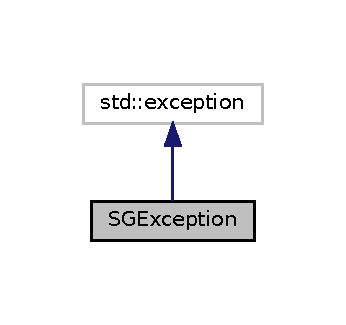
\includegraphics[width=166pt]{classSGException__inherit__graph}
\end{center}
\end{figure}


Collaboration diagram for S\+G\+Exception\+:
\nopagebreak
\begin{figure}[H]
\begin{center}
\leavevmode
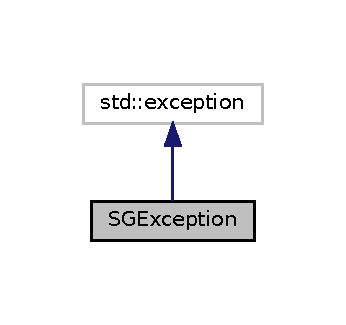
\includegraphics[width=166pt]{classSGException__coll__graph}
\end{center}
\end{figure}
\subsection*{Public Member Functions}
\begin{DoxyCompactItemize}
\item 
\mbox{\Hypertarget{classSGException_a45a1ee37ef4e6d20c9711ee417009889}\label{classSGException_a45a1ee37ef4e6d20c9711ee417009889}} 
\hyperlink{classSGException_a45a1ee37ef4e6d20c9711ee417009889}{S\+G\+Exception} (\hyperlink{namespaceSG_a671df7c720746d1e853deee02bad6411}{S\+G\+::\+E\+X\+C\+E\+P\+T\+I\+O\+N\+\_\+\+T\+Y\+PE} \+\_\+type=\hyperlink{namespaceSG_a671df7c720746d1e853deee02bad6411a0c0f6f82ce3e38637b36fdf4fe34d79f}{S\+G\+::\+D\+E\+F\+A\+U\+LT})
\begin{DoxyCompactList}\small\item\em Constructor for new \hyperlink{classSGException}{S\+G\+Exception}. \end{DoxyCompactList}\item 
\mbox{\Hypertarget{classSGException_a5a43e290f591ee26d0674d3455f6c144}\label{classSGException_a5a43e290f591ee26d0674d3455f6c144}} 
virtual const char $\ast$ \hyperlink{classSGException_a5a43e290f591ee26d0674d3455f6c144}{what} () const  throw ()
\begin{DoxyCompactList}\small\item\em Returns the message corresponding to the Exception\+Type. \end{DoxyCompactList}\item 
\mbox{\Hypertarget{classSGException_afd64ecf52ffdf1b2f8c20103a73cbc60}\label{classSGException_afd64ecf52ffdf1b2f8c20103a73cbc60}} 
\hyperlink{namespaceSG_a671df7c720746d1e853deee02bad6411}{S\+G\+::\+E\+X\+C\+E\+P\+T\+I\+O\+N\+\_\+\+T\+Y\+PE} \hyperlink{classSGException_afd64ecf52ffdf1b2f8c20103a73cbc60}{get\+Type} () const
\begin{DoxyCompactList}\small\item\em Returns the type of the exception. \end{DoxyCompactList}\end{DoxyCompactItemize}
\subsection*{Private Attributes}
\begin{DoxyCompactItemize}
\item 
\mbox{\Hypertarget{classSGException_aa010288cdfd8ff0ef068b23c614601b6}\label{classSGException_aa010288cdfd8ff0ef068b23c614601b6}} 
\hyperlink{namespaceSG_a671df7c720746d1e853deee02bad6411}{S\+G\+::\+E\+X\+C\+E\+P\+T\+I\+O\+N\+\_\+\+T\+Y\+PE} \hyperlink{classSGException_aa010288cdfd8ff0ef068b23c614601b6}{type}
\begin{DoxyCompactList}\small\item\em Flag that indicates the type of error encountered. \end{DoxyCompactList}\end{DoxyCompactItemize}


\subsection{Detailed Description}
S\+G\+Solve specific exceptions. 

This class is derived from std\+::exception and handles special messages that are informative about abnormal behavior in \hyperlink{classSGSolver}{S\+G\+Solver} and associated classes. \begin{Desc}
\item[Examples\+: ]\par
\hyperlink{pd_twostate_8cpp-example}{pd\+\_\+twostate.\+cpp}.\end{Desc}


The documentation for this class was generated from the following files\+:\begin{DoxyCompactItemize}
\item 
src/hpp/sgexception.\+hpp\item 
src/cpp/sgexception.\+cpp\end{DoxyCompactItemize}

\hypertarget{classSGGame}{}\section{S\+G\+Game Class Reference}
\label{classSGGame}\index{S\+G\+Game@{S\+G\+Game}}


Describes a stochastic game.  




{\ttfamily \#include $<$sggame.\+hpp$>$}



Collaboration diagram for S\+G\+Game\+:
\nopagebreak
\begin{figure}[H]
\begin{center}
\leavevmode
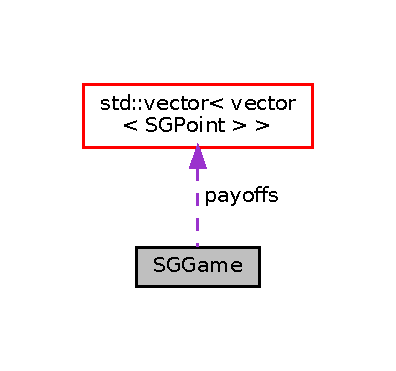
\includegraphics[width=190pt]{classSGGame__coll__graph}
\end{center}
\end{figure}
\subsection*{Public Member Functions}
\begin{DoxyCompactItemize}
\item 
\mbox{\Hypertarget{classSGGame_a935fc76700c675f842dc1666ffe2e8f7}\label{classSGGame_a935fc76700c675f842dc1666ffe2e8f7}} 
\hyperlink{classSGGame_a935fc76700c675f842dc1666ffe2e8f7}{S\+G\+Game} ()
\begin{DoxyCompactList}\small\item\em Default constructor. \end{DoxyCompactList}\item 
\hyperlink{classSGGame_a0b85bb1b3a04539bef72dadc7e170b2f}{S\+G\+Game} (const \hyperlink{classSGAbstractGame}{S\+G\+Abstract\+Game} \&game)
\begin{DoxyCompactList}\small\item\em Converts an \hyperlink{classSGAbstractGame}{S\+G\+Abstract\+Game} into a \hyperlink{classSGGame}{S\+G\+Game}. \end{DoxyCompactList}\item 
\hyperlink{classSGGame_ad881fb3f3db38d4b7c2ea0beb7181fc0}{S\+G\+Game} (double \+\_\+delta, int \+\_\+num\+States, const vector$<$ vector$<$ int $>$ $>$ \&\+\_\+num\+Actions, const vector$<$ vector$<$ vector$<$ double $>$ $>$ $>$ \&\+\_\+payoffs, const vector$<$ vector$<$ vector$<$ double $>$ $>$ $>$ \&\+\_\+probabilities)
\begin{DoxyCompactList}\small\item\em Constructor excluding eq\+Actions. \end{DoxyCompactList}\item 
\mbox{\Hypertarget{classSGGame_ad4d48551202bda3c56f8860a24f04260}\label{classSGGame_ad4d48551202bda3c56f8860a24f04260}} 
\hyperlink{classSGGame_ad4d48551202bda3c56f8860a24f04260}{S\+G\+Game} (double \+\_\+delta, int \+\_\+num\+States, const vector$<$ vector$<$ int $>$ $>$ \&\+\_\+num\+Actions, const vector$<$ vector$<$ vector$<$ double $>$ $>$ $>$ \&\+\_\+payoffs, const vector$<$ vector$<$ vector$<$ double $>$ $>$ $>$ \&\+\_\+probabilities, const vector$<$ bool $>$ \&\+\_\+unconstrained)
\begin{DoxyCompactList}\small\item\em Constructor customizing unconstrained. \end{DoxyCompactList}\item 
\hyperlink{classSGGame_abf23f0bd27cc79e44bdae273ef8a7735}{S\+G\+Game} (double \+\_\+delta, int \+\_\+num\+States, const vector$<$ vector$<$ int $>$ $>$ \&\+\_\+num\+Actions, const vector$<$ vector$<$ vector$<$ double $>$ $>$ $>$ \&\+\_\+payoffs, const vector$<$ vector$<$ vector$<$ double $>$ $>$ $>$ \&\+\_\+probabilities, const vector$<$ vector$<$ bool $>$ $>$ \&\+\_\+eq\+Actions, const vector$<$ bool $>$ \&\+\_\+unconstrained)
\begin{DoxyCompactList}\small\item\em Constructor customizing equilibrium actions. \end{DoxyCompactList}\item 
\hyperlink{classSGGame_af6715eb62a0133849bbe9fe60fe113ab}{S\+G\+Game} (int \+\_\+num\+Players, double \+\_\+delta, int \+\_\+num\+States, const vector$<$ vector$<$ int $>$ $>$ \&\+\_\+num\+Actions, const vector$<$ vector$<$ vector$<$ double $>$ $>$ $>$ \&\+\_\+payoffs, const vector$<$ vector$<$ vector$<$ double $>$ $>$ $>$ \&\+\_\+probabilities, const vector$<$ vector$<$ bool $>$ $>$ \&\+\_\+eq\+Actions, const vector$<$ bool $>$ \&\+\_\+unconstrained)
\begin{DoxyCompactList}\small\item\em Constructor with custom num\+Players. \end{DoxyCompactList}\item 
\mbox{\Hypertarget{classSGGame_aefa61117ee6c117c297791f976b36324}\label{classSGGame_aefa61117ee6c117c297791f976b36324}} 
double \hyperlink{classSGGame_aefa61117ee6c117c297791f976b36324}{get\+Delta} () const
\begin{DoxyCompactList}\small\item\em Returns \hyperlink{classSGGame_a5031fc31f8009c19901c0930224e0465}{S\+G\+Game\+::delta}, the discount factor. \end{DoxyCompactList}\item 
\mbox{\Hypertarget{classSGGame_aaecc5512e85b0c360d4c462d3f84eae0}\label{classSGGame_aaecc5512e85b0c360d4c462d3f84eae0}} 
int \hyperlink{classSGGame_aaecc5512e85b0c360d4c462d3f84eae0}{get\+Num\+Players} () const
\begin{DoxyCompactList}\small\item\em Returns \hyperlink{classSGGame_a6f02e3f92db6a3c5d2d9076dcb7b6d61}{S\+G\+Game\+::num\+Players}, the number of players. \end{DoxyCompactList}\item 
\mbox{\Hypertarget{classSGGame_a1cbb93f4557f71df9d7bffcfeb8ff51c}\label{classSGGame_a1cbb93f4557f71df9d7bffcfeb8ff51c}} 
int \hyperlink{classSGGame_a1cbb93f4557f71df9d7bffcfeb8ff51c}{get\+Num\+States} () const
\begin{DoxyCompactList}\small\item\em Returns the number of states. \end{DoxyCompactList}\item 
\mbox{\Hypertarget{classSGGame_acfd5f0817645a9adf9474552aca4f62e}\label{classSGGame_acfd5f0817645a9adf9474552aca4f62e}} 
const vector$<$ vector$<$ int $>$ $>$ \& \hyperlink{classSGGame_acfd5f0817645a9adf9474552aca4f62e}{get\+Num\+Actions} () const
\begin{DoxyCompactList}\small\item\em Sets the argument \+\_\+num\+Actions equal to \hyperlink{classSGGame_acebe94d195ffb67f92925bcd4c26d1a9}{S\+G\+Game\+::num\+Actions}. \end{DoxyCompactList}\item 
const vector$<$ int $>$ \& \hyperlink{classSGGame_a22f9effebebb711e2f174c4a95a49420}{get\+Num\+Actions\+\_\+total} () const
\item 
\mbox{\Hypertarget{classSGGame_a0d2fef107bd38ad4c848fd35b0ed5ddf}\label{classSGGame_a0d2fef107bd38ad4c848fd35b0ed5ddf}} 
const vector$<$ vector$<$ vector$<$ double $>$ $>$ $>$ \& \hyperlink{classSGGame_a0d2fef107bd38ad4c848fd35b0ed5ddf}{get\+Probabilities} () const
\begin{DoxyCompactList}\small\item\em Returns a const reference to probabilities. \end{DoxyCompactList}\item 
\mbox{\Hypertarget{classSGGame_a37036f4f8389a68c53b12eb75c1eb7af}\label{classSGGame_a37036f4f8389a68c53b12eb75c1eb7af}} 
const vector$<$ vector$<$ \hyperlink{classSGPoint}{S\+G\+Point} $>$ $>$ \& \hyperlink{classSGGame_a37036f4f8389a68c53b12eb75c1eb7af}{get\+Payoffs} () const
\begin{DoxyCompactList}\small\item\em Returns a const reference to the payoffs. \end{DoxyCompactList}\item 
\mbox{\Hypertarget{classSGGame_a5cbb8386739f0ddcb6bc1666dcba3b7b}\label{classSGGame_a5cbb8386739f0ddcb6bc1666dcba3b7b}} 
const vector$<$ vector$<$ bool $>$ $>$ \& \hyperlink{classSGGame_a5cbb8386739f0ddcb6bc1666dcba3b7b}{get\+Equilibrium\+Actions} () const
\begin{DoxyCompactList}\small\item\em Returns a const reference to the equilibrium actions. \end{DoxyCompactList}\item 
void \hyperlink{classSGGame_a32293b2ba26d2a8cd264e3b9e7559d22}{get\+Payoff\+Bounds} (\hyperlink{classSGPoint}{S\+G\+Point} \&UB, \hyperlink{classSGPoint}{S\+G\+Point} \&LB) const
\item 
\mbox{\Hypertarget{classSGGame_aa32846060a1f8a9b9fc0419a1c1c0510}\label{classSGGame_aa32846060a1f8a9b9fc0419a1c1c0510}} 
const vector$<$ bool $>$ \& \hyperlink{classSGGame_aa32846060a1f8a9b9fc0419a1c1c0510}{get\+Constrained} () const
\begin{DoxyCompactList}\small\item\em Returns the unconstrained vector. \end{DoxyCompactList}\item 
bool \hyperlink{classSGGame_ad5879878c647da7040940469b56b9595}{set\+Discount\+Factor} (double new\+Delta)
\begin{DoxyCompactList}\small\item\em Set discount factor. \end{DoxyCompactList}\item 
bool \hyperlink{classSGGame_a36b2269c87d27ab3e0278ad44b6bbddc}{set\+Payoff} (int state, int action, int player, double payoff)
\begin{DoxyCompactList}\small\item\em Set payoffs. \end{DoxyCompactList}\item 
bool \hyperlink{classSGGame_afcc31eacca8f294d349905d52c9a5f64}{set\+Probability} (int state, int action, int new\+State, double prob)
\begin{DoxyCompactList}\small\item\em Set probability. \end{DoxyCompactList}\item 
\mbox{\Hypertarget{classSGGame_a5526a6eb4c4fbb9bc6ff3334e411fbf1}\label{classSGGame_a5526a6eb4c4fbb9bc6ff3334e411fbf1}} 
bool \hyperlink{classSGGame_a5526a6eb4c4fbb9bc6ff3334e411fbf1}{set\+Constrained} (const vector$<$ bool $>$ \&\+\_\+unconstrained)
\begin{DoxyCompactList}\small\item\em Sets whether or not players are incentive constrained. \end{DoxyCompactList}\item 
bool \hyperlink{classSGGame_a2b3ddf3f5dfca8514cba1933205c5ec3}{add\+Action} (int state, int player, int position)
\begin{DoxyCompactList}\small\item\em Adds a new action. \end{DoxyCompactList}\item 
\mbox{\Hypertarget{classSGGame_a97999290a05ab0427fd36d0a2a737944}\label{classSGGame_a97999290a05ab0427fd36d0a2a737944}} 
bool \hyperlink{classSGGame_a97999290a05ab0427fd36d0a2a737944}{remove\+Action} (int state, int player, int action)
\begin{DoxyCompactList}\small\item\em Removes the given action. \end{DoxyCompactList}\item 
bool \hyperlink{classSGGame_a0e4ea56b9e9787dca697782cbedc76d6}{add\+State} (int position)
\begin{DoxyCompactList}\small\item\em Adds a new state. \end{DoxyCompactList}\item 
\mbox{\Hypertarget{classSGGame_ae4930c4311ee2f7a814400e3e50123a8}\label{classSGGame_ae4930c4311ee2f7a814400e3e50123a8}} 
bool \hyperlink{classSGGame_ae4930c4311ee2f7a814400e3e50123a8}{remove\+State} (int state)
\begin{DoxyCompactList}\small\item\em Removes the given state. \end{DoxyCompactList}\item 
\mbox{\Hypertarget{classSGGame_a4bf2a75864749594145cbd2194ebadd4}\label{classSGGame_a4bf2a75864749594145cbd2194ebadd4}} 
bool \hyperlink{classSGGame_a4bf2a75864749594145cbd2194ebadd4}{transition\+Probs\+Sum\+To\+One} () const
\begin{DoxyCompactList}\small\item\em Check if transition probabilities sum to one. \end{DoxyCompactList}\end{DoxyCompactItemize}
\subsection*{Static Public Member Functions}
\begin{DoxyCompactItemize}
\item 
\mbox{\Hypertarget{classSGGame_aaccf18a3663ec99360e5b6e64f2bf6e2}\label{classSGGame_aaccf18a3663ec99360e5b6e64f2bf6e2}} 
static void \hyperlink{classSGGame_aaccf18a3663ec99360e5b6e64f2bf6e2}{save} (const \hyperlink{classSGGame}{S\+G\+Game} \&game, const char $\ast$filename)
\begin{DoxyCompactList}\small\item\em Static method for saving an \hyperlink{classSGGame}{S\+G\+Game} object to the file filename. \end{DoxyCompactList}\item 
\mbox{\Hypertarget{classSGGame_ac1dc35b84318448efc37b80afe210170}\label{classSGGame_ac1dc35b84318448efc37b80afe210170}} 
static void \hyperlink{classSGGame_ac1dc35b84318448efc37b80afe210170}{load} (\hyperlink{classSGGame}{S\+G\+Game} \&game, const char $\ast$filename)
\begin{DoxyCompactList}\small\item\em Static method for loading an \hyperlink{classSGGame}{S\+G\+Game} object from the file filename. \end{DoxyCompactList}\end{DoxyCompactItemize}
\subsection*{Private Member Functions}
\begin{DoxyCompactItemize}
\item 
\mbox{\Hypertarget{classSGGame_a383c8f7ec881befac40d6e45c7e1b775}\label{classSGGame_a383c8f7ec881befac40d6e45c7e1b775}} 
{\footnotesize template$<$class Archive $>$ }\\void \hyperlink{classSGGame_a383c8f7ec881befac40d6e45c7e1b775}{serialize} (Archive \&ar, const unsigned int version)
\begin{DoxyCompactList}\small\item\em Serializes the game using boost. \end{DoxyCompactList}\end{DoxyCompactItemize}
\subsection*{Private Attributes}
\begin{DoxyCompactItemize}
\item 
double \hyperlink{classSGGame_a5031fc31f8009c19901c0930224e0465}{delta}
\item 
int \hyperlink{classSGGame_a6f02e3f92db6a3c5d2d9076dcb7b6d61}{num\+Players}
\item 
int \hyperlink{classSGGame_ae7b105b2fe9ee277d38e518223dd0482}{num\+States}
\item 
vector$<$ vector$<$ int $>$ $>$ \hyperlink{classSGGame_acebe94d195ffb67f92925bcd4c26d1a9}{num\+Actions}
\item 
vector$<$ int $>$ \hyperlink{classSGGame_a3b219a37177b5b8b38737f570e419429}{num\+Actions\+\_\+total}
\item 
vector$<$ vector$<$ \hyperlink{classSGPoint}{S\+G\+Point} $>$ $>$ \hyperlink{classSGGame_aad28dd39c6359e772286a938a948634c}{payoffs}
\item 
vector$<$ vector$<$ vector$<$ double $>$ $>$ $>$ \hyperlink{classSGGame_a167a281b11d524cb4a11dbaff3e9de68}{probabilities}
\item 
vector$<$ vector$<$ bool $>$ $>$ \hyperlink{classSGGame_aacb0878b1e95ef3ff42cb88ac617c0b8}{eq\+Actions}
\item 
vector$<$ bool $>$ \hyperlink{classSGGame_a528852e11bd68322535d7f24a41eca20}{unconstrained}
\end{DoxyCompactItemize}
\subsection*{Friends}
\begin{DoxyCompactItemize}
\item 
\mbox{\Hypertarget{classSGGame_ac98d07dd8f7b70e16ccb9a01abf56b9c}\label{classSGGame_ac98d07dd8f7b70e16ccb9a01abf56b9c}} 
class {\bfseries boost\+::serialization\+::access}
\item 
\mbox{\Hypertarget{classSGGame_a8b0e5d2bebfed7e7e032366bb49bc5f1}\label{classSGGame_a8b0e5d2bebfed7e7e032366bb49bc5f1}} 
class {\bfseries S\+G\+Solver}
\end{DoxyCompactItemize}


\subsection{Detailed Description}
Describes a stochastic game. 

This class contains members that describe a stochastic game. \begin{Desc}
\item[Examples\+: ]\par
\hyperlink{pd_twostate_8cpp-example}{pd\+\_\+twostate.\+cpp}, and \hyperlink{risksharing_maxminmax_8cpp-example}{risksharing\+\_\+maxminmax.\+cpp}.\end{Desc}


\subsection{Constructor \& Destructor Documentation}
\mbox{\Hypertarget{classSGGame_a0b85bb1b3a04539bef72dadc7e170b2f}\label{classSGGame_a0b85bb1b3a04539bef72dadc7e170b2f}} 
\index{S\+G\+Game@{S\+G\+Game}!S\+G\+Game@{S\+G\+Game}}
\index{S\+G\+Game@{S\+G\+Game}!S\+G\+Game@{S\+G\+Game}}
\subsubsection{\texorpdfstring{S\+G\+Game()}{SGGame()}\hspace{0.1cm}{\footnotesize\ttfamily [1/4]}}
{\footnotesize\ttfamily S\+G\+Game\+::\+S\+G\+Game (\begin{DoxyParamCaption}\item[{const \hyperlink{classSGAbstractGame}{S\+G\+Abstract\+Game} \&}]{game }\end{DoxyParamCaption})}



Converts an \hyperlink{classSGAbstractGame}{S\+G\+Abstract\+Game} into a \hyperlink{classSGGame}{S\+G\+Game}. 

The user can derive their own class from \hyperlink{classSGAbstractGame}{S\+G\+Abstract\+Game}, and then pass the derived object to the \hyperlink{classSGGame}{S\+G\+Game} constructor. This constructor essentially copies the data from the user defined payoffs and probability methods into arrays. Storing this data in arrays provides for faster access by \hyperlink{classSGApprox}{S\+G\+Approx} and it allows the game to be serialized. See risksharing.\+hpp and risksharing.\+cpp for an example. \mbox{\Hypertarget{classSGGame_ad881fb3f3db38d4b7c2ea0beb7181fc0}\label{classSGGame_ad881fb3f3db38d4b7c2ea0beb7181fc0}} 
\index{S\+G\+Game@{S\+G\+Game}!S\+G\+Game@{S\+G\+Game}}
\index{S\+G\+Game@{S\+G\+Game}!S\+G\+Game@{S\+G\+Game}}
\subsubsection{\texorpdfstring{S\+G\+Game()}{SGGame()}\hspace{0.1cm}{\footnotesize\ttfamily [2/4]}}
{\footnotesize\ttfamily S\+G\+Game\+::\+S\+G\+Game (\begin{DoxyParamCaption}\item[{double}]{\+\_\+delta,  }\item[{int}]{\+\_\+num\+States,  }\item[{const vector$<$ vector$<$ int $>$ $>$ \&}]{\+\_\+num\+Actions,  }\item[{const vector$<$ vector$<$ vector$<$ double $>$ $>$ $>$ \&}]{\+\_\+payoffs,  }\item[{const vector$<$ vector$<$ vector$<$ double $>$ $>$ $>$ \&}]{\+\_\+probabilities }\end{DoxyParamCaption})}



Constructor excluding eq\+Actions. 

$<$ Initializes a game object with all actions being permissible. \mbox{\Hypertarget{classSGGame_abf23f0bd27cc79e44bdae273ef8a7735}\label{classSGGame_abf23f0bd27cc79e44bdae273ef8a7735}} 
\index{S\+G\+Game@{S\+G\+Game}!S\+G\+Game@{S\+G\+Game}}
\index{S\+G\+Game@{S\+G\+Game}!S\+G\+Game@{S\+G\+Game}}
\subsubsection{\texorpdfstring{S\+G\+Game()}{SGGame()}\hspace{0.1cm}{\footnotesize\ttfamily [3/4]}}
{\footnotesize\ttfamily S\+G\+Game\+::\+S\+G\+Game (\begin{DoxyParamCaption}\item[{double}]{\+\_\+delta,  }\item[{int}]{\+\_\+num\+States,  }\item[{const vector$<$ vector$<$ int $>$ $>$ \&}]{\+\_\+num\+Actions,  }\item[{const vector$<$ vector$<$ vector$<$ double $>$ $>$ $>$ \&}]{\+\_\+payoffs,  }\item[{const vector$<$ vector$<$ vector$<$ double $>$ $>$ $>$ \&}]{\+\_\+probabilities,  }\item[{const vector$<$ vector$<$ bool $>$ $>$ \&}]{\+\_\+eq\+Actions,  }\item[{const vector$<$ bool $>$ \&}]{\+\_\+unconstrained }\end{DoxyParamCaption})}



Constructor customizing equilibrium actions. 

$<$ If \+\_\+eq\+Actions is an empty vector, the constructor will initialize it so that all action profiles are allowed. Otherwise, we restrict attention to equilibria in which action profiles in \+\_\+eq\+Actions are used. \mbox{\Hypertarget{classSGGame_af6715eb62a0133849bbe9fe60fe113ab}\label{classSGGame_af6715eb62a0133849bbe9fe60fe113ab}} 
\index{S\+G\+Game@{S\+G\+Game}!S\+G\+Game@{S\+G\+Game}}
\index{S\+G\+Game@{S\+G\+Game}!S\+G\+Game@{S\+G\+Game}}
\subsubsection{\texorpdfstring{S\+G\+Game()}{SGGame()}\hspace{0.1cm}{\footnotesize\ttfamily [4/4]}}
{\footnotesize\ttfamily S\+G\+Game\+::\+S\+G\+Game (\begin{DoxyParamCaption}\item[{int}]{\+\_\+num\+Players,  }\item[{double}]{\+\_\+delta,  }\item[{int}]{\+\_\+num\+States,  }\item[{const vector$<$ vector$<$ int $>$ $>$ \&}]{\+\_\+num\+Actions,  }\item[{const vector$<$ vector$<$ vector$<$ double $>$ $>$ $>$ \&}]{\+\_\+payoffs,  }\item[{const vector$<$ vector$<$ vector$<$ double $>$ $>$ $>$ \&}]{\+\_\+probabilities,  }\item[{const vector$<$ vector$<$ bool $>$ $>$ \&}]{\+\_\+eq\+Actions,  }\item[{const vector$<$ bool $>$ \&}]{\+\_\+unconstrained }\end{DoxyParamCaption})}



Constructor with custom num\+Players. 

$<$ All other constructors eventually call this constructor. 

\subsection{Member Function Documentation}
\mbox{\Hypertarget{classSGGame_a2b3ddf3f5dfca8514cba1933205c5ec3}\label{classSGGame_a2b3ddf3f5dfca8514cba1933205c5ec3}} 
\index{S\+G\+Game@{S\+G\+Game}!add\+Action@{add\+Action}}
\index{add\+Action@{add\+Action}!S\+G\+Game@{S\+G\+Game}}
\subsubsection{\texorpdfstring{add\+Action()}{addAction()}}
{\footnotesize\ttfamily bool S\+G\+Game\+::add\+Action (\begin{DoxyParamCaption}\item[{int}]{state,  }\item[{int}]{player,  }\item[{int}]{position }\end{DoxyParamCaption})}



Adds a new action. 

Adds a new action for the given state and player just after the action at index position. The new action has payoffs initialized to zero, and state remains the same with probability 1. \mbox{\Hypertarget{classSGGame_a0e4ea56b9e9787dca697782cbedc76d6}\label{classSGGame_a0e4ea56b9e9787dca697782cbedc76d6}} 
\index{S\+G\+Game@{S\+G\+Game}!add\+State@{add\+State}}
\index{add\+State@{add\+State}!S\+G\+Game@{S\+G\+Game}}
\subsubsection{\texorpdfstring{add\+State()}{addState()}}
{\footnotesize\ttfamily bool S\+G\+Game\+::add\+State (\begin{DoxyParamCaption}\item[{int}]{position }\end{DoxyParamCaption})}



Adds a new state. 

Inserts a new state after the index position. The new state has one action for each player with payoffs of zero, and the state is absorbing. \mbox{\Hypertarget{classSGGame_a22f9effebebb711e2f174c4a95a49420}\label{classSGGame_a22f9effebebb711e2f174c4a95a49420}} 
\index{S\+G\+Game@{S\+G\+Game}!get\+Num\+Actions\+\_\+total@{get\+Num\+Actions\+\_\+total}}
\index{get\+Num\+Actions\+\_\+total@{get\+Num\+Actions\+\_\+total}!S\+G\+Game@{S\+G\+Game}}
\subsubsection{\texorpdfstring{get\+Num\+Actions\+\_\+total()}{getNumActions\_total()}}
{\footnotesize\ttfamily const vector$<$int$>$\& S\+G\+Game\+::get\+Num\+Actions\+\_\+total (\begin{DoxyParamCaption}{ }\end{DoxyParamCaption}) const\hspace{0.3cm}{\ttfamily [inline]}}

Returns a constant reference to the total number of actions in each state \mbox{\Hypertarget{classSGGame_a32293b2ba26d2a8cd264e3b9e7559d22}\label{classSGGame_a32293b2ba26d2a8cd264e3b9e7559d22}} 
\index{S\+G\+Game@{S\+G\+Game}!get\+Payoff\+Bounds@{get\+Payoff\+Bounds}}
\index{get\+Payoff\+Bounds@{get\+Payoff\+Bounds}!S\+G\+Game@{S\+G\+Game}}
\subsubsection{\texorpdfstring{get\+Payoff\+Bounds()}{getPayoffBounds()}}
{\footnotesize\ttfamily void S\+G\+Game\+::get\+Payoff\+Bounds (\begin{DoxyParamCaption}\item[{\hyperlink{classSGPoint}{S\+G\+Point} \&}]{UB,  }\item[{\hyperlink{classSGPoint}{S\+G\+Point} \&}]{LB }\end{DoxyParamCaption}) const}

Sets the arguments equal to tight upper and lower bounds on the payoffs, respectively. \mbox{\Hypertarget{classSGGame_ad5879878c647da7040940469b56b9595}\label{classSGGame_ad5879878c647da7040940469b56b9595}} 
\index{S\+G\+Game@{S\+G\+Game}!set\+Discount\+Factor@{set\+Discount\+Factor}}
\index{set\+Discount\+Factor@{set\+Discount\+Factor}!S\+G\+Game@{S\+G\+Game}}
\subsubsection{\texorpdfstring{set\+Discount\+Factor()}{setDiscountFactor()}}
{\footnotesize\ttfamily bool S\+G\+Game\+::set\+Discount\+Factor (\begin{DoxyParamCaption}\item[{double}]{new\+Delta }\end{DoxyParamCaption})}



Set discount factor. 

Method for setting the discount factor. \mbox{\Hypertarget{classSGGame_a36b2269c87d27ab3e0278ad44b6bbddc}\label{classSGGame_a36b2269c87d27ab3e0278ad44b6bbddc}} 
\index{S\+G\+Game@{S\+G\+Game}!set\+Payoff@{set\+Payoff}}
\index{set\+Payoff@{set\+Payoff}!S\+G\+Game@{S\+G\+Game}}
\subsubsection{\texorpdfstring{set\+Payoff()}{setPayoff()}}
{\footnotesize\ttfamily bool S\+G\+Game\+::set\+Payoff (\begin{DoxyParamCaption}\item[{int}]{state,  }\item[{int}]{action,  }\item[{int}]{player,  }\item[{double}]{payoff }\end{DoxyParamCaption})}



Set payoffs. 

Method for setting payoffs for the given player, action, and state. \mbox{\Hypertarget{classSGGame_afcc31eacca8f294d349905d52c9a5f64}\label{classSGGame_afcc31eacca8f294d349905d52c9a5f64}} 
\index{S\+G\+Game@{S\+G\+Game}!set\+Probability@{set\+Probability}}
\index{set\+Probability@{set\+Probability}!S\+G\+Game@{S\+G\+Game}}
\subsubsection{\texorpdfstring{set\+Probability()}{setProbability()}}
{\footnotesize\ttfamily bool S\+G\+Game\+::set\+Probability (\begin{DoxyParamCaption}\item[{int}]{state,  }\item[{int}]{action,  }\item[{int}]{new\+State,  }\item[{double}]{prob }\end{DoxyParamCaption})}



Set probability. 

Sets the transition probability from state to new\+State when action is played. 

\subsection{Member Data Documentation}
\mbox{\Hypertarget{classSGGame_a5031fc31f8009c19901c0930224e0465}\label{classSGGame_a5031fc31f8009c19901c0930224e0465}} 
\index{S\+G\+Game@{S\+G\+Game}!delta@{delta}}
\index{delta@{delta}!S\+G\+Game@{S\+G\+Game}}
\subsubsection{\texorpdfstring{delta}{delta}}
{\footnotesize\ttfamily double S\+G\+Game\+::delta\hspace{0.3cm}{\ttfamily [private]}}

The discount factor. \mbox{\Hypertarget{classSGGame_aacb0878b1e95ef3ff42cb88ac617c0b8}\label{classSGGame_aacb0878b1e95ef3ff42cb88ac617c0b8}} 
\index{S\+G\+Game@{S\+G\+Game}!eq\+Actions@{eq\+Actions}}
\index{eq\+Actions@{eq\+Actions}!S\+G\+Game@{S\+G\+Game}}
\subsubsection{\texorpdfstring{eq\+Actions}{eqActions}}
{\footnotesize\ttfamily vector$<$ vector$<$bool$>$ $>$ S\+G\+Game\+::eq\+Actions\hspace{0.3cm}{\ttfamily [private]}}

Indicates which action profiles are allowed to be played on path in each state. By default, initialized to true for all action profiles. Allows one to, for example, look at strongly symmetric equilibria (by first excluding asymmetric action profiles from the lists). Players can always deviate to action profiles which are not allowed on path. \mbox{\Hypertarget{classSGGame_acebe94d195ffb67f92925bcd4c26d1a9}\label{classSGGame_acebe94d195ffb67f92925bcd4c26d1a9}} 
\index{S\+G\+Game@{S\+G\+Game}!num\+Actions@{num\+Actions}}
\index{num\+Actions@{num\+Actions}!S\+G\+Game@{S\+G\+Game}}
\subsubsection{\texorpdfstring{num\+Actions}{numActions}}
{\footnotesize\ttfamily vector$<$ vector$<$int$>$ $>$ S\+G\+Game\+::num\+Actions\hspace{0.3cm}{\ttfamily [private]}}

Gives the number of each player\textquotesingle{}s actions in each state. In particular, player i has num\+Actions\mbox{[}s\mbox{]}\mbox{[}i\mbox{]} actions in state s. Should note that a pair (a1,a2) is mapped into an action profile using the formula a=a1+a2$\ast$num\+Actions\mbox{[}s\mbox{]}\mbox{[}a1\mbox{]}, and generalized to n$>$2. \mbox{\Hypertarget{classSGGame_a3b219a37177b5b8b38737f570e419429}\label{classSGGame_a3b219a37177b5b8b38737f570e419429}} 
\index{S\+G\+Game@{S\+G\+Game}!num\+Actions\+\_\+total@{num\+Actions\+\_\+total}}
\index{num\+Actions\+\_\+total@{num\+Actions\+\_\+total}!S\+G\+Game@{S\+G\+Game}}
\subsubsection{\texorpdfstring{num\+Actions\+\_\+total}{numActions\_total}}
{\footnotesize\ttfamily vector$<$int$>$ S\+G\+Game\+::num\+Actions\+\_\+total\hspace{0.3cm}{\ttfamily [private]}}

Total number of action profiles for each state. \mbox{\Hypertarget{classSGGame_a6f02e3f92db6a3c5d2d9076dcb7b6d61}\label{classSGGame_a6f02e3f92db6a3c5d2d9076dcb7b6d61}} 
\index{S\+G\+Game@{S\+G\+Game}!num\+Players@{num\+Players}}
\index{num\+Players@{num\+Players}!S\+G\+Game@{S\+G\+Game}}
\subsubsection{\texorpdfstring{num\+Players}{numPlayers}}
{\footnotesize\ttfamily int S\+G\+Game\+::num\+Players\hspace{0.3cm}{\ttfamily [private]}}

The number of players. \mbox{\Hypertarget{classSGGame_ae7b105b2fe9ee277d38e518223dd0482}\label{classSGGame_ae7b105b2fe9ee277d38e518223dd0482}} 
\index{S\+G\+Game@{S\+G\+Game}!num\+States@{num\+States}}
\index{num\+States@{num\+States}!S\+G\+Game@{S\+G\+Game}}
\subsubsection{\texorpdfstring{num\+States}{numStates}}
{\footnotesize\ttfamily int S\+G\+Game\+::num\+States\hspace{0.3cm}{\ttfamily [private]}}

The number of states, must be at least 1. \mbox{\Hypertarget{classSGGame_aad28dd39c6359e772286a938a948634c}\label{classSGGame_aad28dd39c6359e772286a938a948634c}} 
\index{S\+G\+Game@{S\+G\+Game}!payoffs@{payoffs}}
\index{payoffs@{payoffs}!S\+G\+Game@{S\+G\+Game}}
\subsubsection{\texorpdfstring{payoffs}{payoffs}}
{\footnotesize\ttfamily vector$<$ vector$<$\hyperlink{classSGPoint}{S\+G\+Point}$>$ $>$ S\+G\+Game\+::payoffs\hspace{0.3cm}{\ttfamily [private]}}

Gives the payoffs of the players as a function of the action profile. In particular, payoffs\mbox{[}s\mbox{]}\mbox{[}a\mbox{]}\mbox{[}i\mbox{]} are player i\textquotesingle{}s payoffs in state s when action profile a is played. \mbox{\Hypertarget{classSGGame_a167a281b11d524cb4a11dbaff3e9de68}\label{classSGGame_a167a281b11d524cb4a11dbaff3e9de68}} 
\index{S\+G\+Game@{S\+G\+Game}!probabilities@{probabilities}}
\index{probabilities@{probabilities}!S\+G\+Game@{S\+G\+Game}}
\subsubsection{\texorpdfstring{probabilities}{probabilities}}
{\footnotesize\ttfamily vector$<$ vector$<$ vector$<$double$>$ $>$ $>$ S\+G\+Game\+::probabilities\hspace{0.3cm}{\ttfamily [private]}}

State transition probabilities\+: probabilities\mbox{[}s\mbox{]}\mbox{[}a\mbox{]}\mbox{[}s\textquotesingle{}\mbox{]} is the probability of transitioning to state s\textquotesingle{} when action profile a is played in state s. \mbox{\Hypertarget{classSGGame_a528852e11bd68322535d7f24a41eca20}\label{classSGGame_a528852e11bd68322535d7f24a41eca20}} 
\index{S\+G\+Game@{S\+G\+Game}!unconstrained@{unconstrained}}
\index{unconstrained@{unconstrained}!S\+G\+Game@{S\+G\+Game}}
\subsubsection{\texorpdfstring{unconstrained}{unconstrained}}
{\footnotesize\ttfamily vector$<$bool$>$ S\+G\+Game\+::unconstrained\hspace{0.3cm}{\ttfamily [private]}}

If unconstrained\mbox{[}i\mbox{]}=true, the algorithm will not impose incentive compatibility as a constraint for player i. 

The documentation for this class was generated from the following files\+:\begin{DoxyCompactItemize}
\item 
src/hpp/sggame.\+hpp\item 
src/cpp/sggame.\+cpp\end{DoxyCompactItemize}

\hypertarget{classSGIteration}{}\section{S\+G\+Iteration Class Reference}
\label{classSGIteration}\index{S\+G\+Iteration@{S\+G\+Iteration}}


Stores data on the behavior of \hyperlink{classSGApprox_a9cf7330f7cab3f454b0850e778d132fa}{S\+G\+Approx\+::generate()}  




{\ttfamily \#include $<$sgiteration.\+hpp$>$}



Collaboration diagram for S\+G\+Iteration\+:
\nopagebreak
\begin{figure}[H]
\begin{center}
\leavevmode
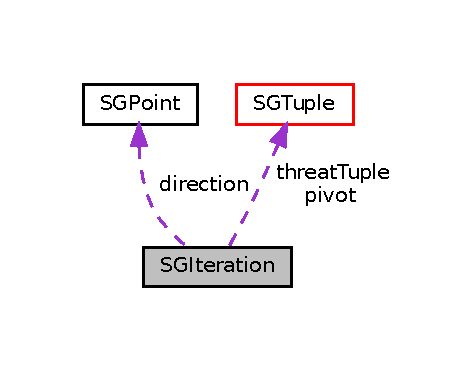
\includegraphics[width=228pt]{classSGIteration__coll__graph}
\end{center}
\end{figure}
\subsection*{Public Member Functions}
\begin{DoxyCompactItemize}
\item 
\mbox{\Hypertarget{classSGIteration_aa47645b3a728b2ca55ad2e7d17c5c488}\label{classSGIteration_aa47645b3a728b2ca55ad2e7d17c5c488}} 
\hyperlink{classSGIteration_aa47645b3a728b2ca55ad2e7d17c5c488}{S\+G\+Iteration} ()
\begin{DoxyCompactList}\small\item\em Default constructor. \end{DoxyCompactList}\item 
\hyperlink{classSGIteration_a4ac425cc85882c11443ef43601efd80b}{S\+G\+Iteration} (const \hyperlink{classSGApprox}{S\+G\+Approx} \&approx, bool store\+Actions=true)
\item 
\mbox{\Hypertarget{classSGIteration_a84d8aaef35b4a93f555cf1e0d8e5b964}\label{classSGIteration_a84d8aaef35b4a93f555cf1e0d8e5b964}} 
int \hyperlink{classSGIteration_a84d8aaef35b4a93f555cf1e0d8e5b964}{get\+Iteration} () const
\begin{DoxyCompactList}\small\item\em Get method for the iteration. \end{DoxyCompactList}\item 
\mbox{\Hypertarget{classSGIteration_af8b2fc2937e7c81248009904ffd0c14b}\label{classSGIteration_af8b2fc2937e7c81248009904ffd0c14b}} 
int \hyperlink{classSGIteration_af8b2fc2937e7c81248009904ffd0c14b}{get\+Revolution} () const
\begin{DoxyCompactList}\small\item\em Get method for the revolution. \end{DoxyCompactList}\item 
\mbox{\Hypertarget{classSGIteration_afd87a05e0df65e9361044f5cef1c5cc6}\label{classSGIteration_afd87a05e0df65e9361044f5cef1c5cc6}} 
int \hyperlink{classSGIteration_afd87a05e0df65e9361044f5cef1c5cc6}{get\+Num\+Extreme\+Tuples} () const
\begin{DoxyCompactList}\small\item\em Get method for the number of extreme tuples. \end{DoxyCompactList}\item 
\mbox{\Hypertarget{classSGIteration_a4a9c13016c8f6ffd0238e95c0076011c}\label{classSGIteration_a4a9c13016c8f6ffd0238e95c0076011c}} 
const \hyperlink{classSGTuple}{S\+G\+Tuple} \& \hyperlink{classSGIteration_a4a9c13016c8f6ffd0238e95c0076011c}{get\+Pivot} () const
\begin{DoxyCompactList}\small\item\em Get method for the current pivot. \end{DoxyCompactList}\item 
\mbox{\Hypertarget{classSGIteration_a684abe31e6b4a3bdf94be1b3fdc6cc66}\label{classSGIteration_a684abe31e6b4a3bdf94be1b3fdc6cc66}} 
const \hyperlink{classSGPoint}{S\+G\+Point} \& \hyperlink{classSGIteration_a684abe31e6b4a3bdf94be1b3fdc6cc66}{get\+Direction} () const
\begin{DoxyCompactList}\small\item\em Get method for the current direction. \end{DoxyCompactList}\item 
\mbox{\Hypertarget{classSGIteration_afb42582d89f27f44d7e76a2f4ff8a684}\label{classSGIteration_afb42582d89f27f44d7e76a2f4ff8a684}} 
const vector$<$ vector$<$ \hyperlink{classSGBaseAction}{S\+G\+Base\+Action} $>$ $>$ \& \hyperlink{classSGIteration_afb42582d89f27f44d7e76a2f4ff8a684}{get\+Actions} () const
\begin{DoxyCompactList}\small\item\em Get method for the actions available at the current iteration. \end{DoxyCompactList}\item 
\mbox{\Hypertarget{classSGIteration_a68b79d82fca24ae8fd10ef1192d9a89e}\label{classSGIteration_a68b79d82fca24ae8fd10ef1192d9a89e}} 
int \hyperlink{classSGIteration_a68b79d82fca24ae8fd10ef1192d9a89e}{get\+Best\+State} () const
\begin{DoxyCompactList}\small\item\em Get method for the best state. \end{DoxyCompactList}\item 
\mbox{\Hypertarget{classSGIteration_a7ea9824327feae3242915ee676b66ae5}\label{classSGIteration_a7ea9824327feae3242915ee676b66ae5}} 
int \hyperlink{classSGIteration_a7ea9824327feae3242915ee676b66ae5}{get\+Best\+Action} () const
\begin{DoxyCompactList}\small\item\em Get method for the best action. \end{DoxyCompactList}\item 
\mbox{\Hypertarget{classSGIteration_a6495e67cc2fd614335416e50aa725955}\label{classSGIteration_a6495e67cc2fd614335416e50aa725955}} 
\hyperlink{namespaceSG_a139e4dec41ea0f38aae1f93f60cfff60}{S\+G\+::\+Regime} \hyperlink{classSGIteration_a6495e67cc2fd614335416e50aa725955}{get\+Regime} () const
\begin{DoxyCompactList}\small\item\em Get method for the regime corresponding to the best direction. \end{DoxyCompactList}\item 
\mbox{\Hypertarget{classSGIteration_a2b8d87df8e7c5cc825938c0f57368c21}\label{classSGIteration_a2b8d87df8e7c5cc825938c0f57368c21}} 
const vector$<$ int $>$ \& \hyperlink{classSGIteration_a2b8d87df8e7c5cc825938c0f57368c21}{get\+Action\+Tuple} () const
\begin{DoxyCompactList}\small\item\em Get method for the action tuple. \end{DoxyCompactList}\item 
\mbox{\Hypertarget{classSGIteration_aefc7abf8f1819c34acf04f313d8908d2}\label{classSGIteration_aefc7abf8f1819c34acf04f313d8908d2}} 
const vector$<$ \hyperlink{namespaceSG_a139e4dec41ea0f38aae1f93f60cfff60}{S\+G\+::\+Regime} $>$ \& \hyperlink{classSGIteration_aefc7abf8f1819c34acf04f313d8908d2}{get\+Regime\+Tuple} () const
\begin{DoxyCompactList}\small\item\em Get method for the regime tuple. \end{DoxyCompactList}\item 
\mbox{\Hypertarget{classSGIteration_a1480e56c07b27be906de438b105945da}\label{classSGIteration_a1480e56c07b27be906de438b105945da}} 
const \hyperlink{classSGTuple}{S\+G\+Tuple} \& \hyperlink{classSGIteration_a1480e56c07b27be906de438b105945da}{get\+Threat\+Tuple} () const
\begin{DoxyCompactList}\small\item\em Get method for the current threat tuple. \end{DoxyCompactList}\item 
\mbox{\Hypertarget{classSGIteration_a19860e6d2af702df4ce47e36d4d43ec5}\label{classSGIteration_a19860e6d2af702df4ce47e36d4d43ec5}} 
{\footnotesize template$<$class Archive $>$ }\\void \hyperlink{classSGIteration_a19860e6d2af702df4ce47e36d4d43ec5}{serialize} (Archive \&ar, const unsigned int version)
\begin{DoxyCompactList}\small\item\em Serialize the iteration using Boost. \end{DoxyCompactList}\end{DoxyCompactItemize}
\subsection*{Private Attributes}
\begin{DoxyCompactItemize}
\item 
int \hyperlink{classSGIteration_a44a4f9e3cb074181292ae816b2c28d9e}{iteration}
\item 
int \hyperlink{classSGIteration_a21cc5c4fc7c40ff444ac7e3743c13940}{revolution}
\item 
int \hyperlink{classSGIteration_a14ecfb94b3111911d9b0ef545f72e88d}{num\+Extreme\+Tuples}
\item 
\hyperlink{classSGTuple}{S\+G\+Tuple} \hyperlink{classSGIteration_abdae7d336968af3515e7d9590cbcc46d}{pivot}
\item 
\hyperlink{classSGPoint}{S\+G\+Point} \hyperlink{classSGIteration_ac35e7e3049cd60c695a366cb8f75db37}{direction}
\item 
vector$<$ vector$<$ \hyperlink{classSGBaseAction}{S\+G\+Base\+Action} $>$ $>$ \hyperlink{classSGIteration_a5b5fcd6440b8dbcc6a8ded9f81699337}{actions}
\item 
\mbox{\Hypertarget{classSGIteration_a16f16d027bab6baffeee1f4cadb3ce8f}\label{classSGIteration_a16f16d027bab6baffeee1f4cadb3ce8f}} 
int \hyperlink{classSGIteration_a16f16d027bab6baffeee1f4cadb3ce8f}{best\+State}
\begin{DoxyCompactList}\small\item\em The state that generated the best direction. \end{DoxyCompactList}\item 
\mbox{\Hypertarget{classSGIteration_a71c4414688b49fe6205fe8d90febd5b5}\label{classSGIteration_a71c4414688b49fe6205fe8d90febd5b5}} 
int \hyperlink{classSGIteration_a71c4414688b49fe6205fe8d90febd5b5}{best\+Action}
\begin{DoxyCompactList}\small\item\em The action that generated the best direction. \end{DoxyCompactList}\item 
\mbox{\Hypertarget{classSGIteration_a0dae9bbd62ac96335698290c2866efc8}\label{classSGIteration_a0dae9bbd62ac96335698290c2866efc8}} 
\hyperlink{namespaceSG_a139e4dec41ea0f38aae1f93f60cfff60}{S\+G\+::\+Regime} \hyperlink{classSGIteration_a0dae9bbd62ac96335698290c2866efc8}{regime}
\begin{DoxyCompactList}\small\item\em True if the best direction was non-\/binding. \end{DoxyCompactList}\item 
\mbox{\Hypertarget{classSGIteration_ade2d5d602a23f5a83a76283fa4dcec87}\label{classSGIteration_ade2d5d602a23f5a83a76283fa4dcec87}} 
vector$<$ int $>$ \hyperlink{classSGIteration_ade2d5d602a23f5a83a76283fa4dcec87}{action\+Tuple}
\begin{DoxyCompactList}\small\item\em The current action tuple. \end{DoxyCompactList}\item 
\mbox{\Hypertarget{classSGIteration_a81c6328aac47bae67d8d7fdd175af738}\label{classSGIteration_a81c6328aac47bae67d8d7fdd175af738}} 
vector$<$ \hyperlink{namespaceSG_a139e4dec41ea0f38aae1f93f60cfff60}{S\+G\+::\+Regime} $>$ \hyperlink{classSGIteration_a81c6328aac47bae67d8d7fdd175af738}{regime\+Tuple}
\begin{DoxyCompactList}\small\item\em The states in which IC constraints are not binding. \end{DoxyCompactList}\item 
\mbox{\Hypertarget{classSGIteration_acaf191aa3e5adddbf1052602c927d03f}\label{classSGIteration_acaf191aa3e5adddbf1052602c927d03f}} 
\hyperlink{classSGTuple}{S\+G\+Tuple} \hyperlink{classSGIteration_acaf191aa3e5adddbf1052602c927d03f}{threat\+Tuple}
\begin{DoxyCompactList}\small\item\em The current threat tuple. \end{DoxyCompactList}\end{DoxyCompactItemize}
\subsection*{Friends}
\begin{DoxyCompactItemize}
\item 
\mbox{\Hypertarget{classSGIteration_ac98d07dd8f7b70e16ccb9a01abf56b9c}\label{classSGIteration_ac98d07dd8f7b70e16ccb9a01abf56b9c}} 
class \hyperlink{classSGIteration_ac98d07dd8f7b70e16ccb9a01abf56b9c}{boost\+::serialization\+::access}
\begin{DoxyCompactList}\small\item\em Serializes the \hyperlink{classSGIteration}{S\+G\+Iteration} object using boost. \end{DoxyCompactList}\end{DoxyCompactItemize}


\subsection{Detailed Description}
Stores data on the behavior of \hyperlink{classSGApprox_a9cf7330f7cab3f454b0850e778d132fa}{S\+G\+Approx\+::generate()} 

This class records information on each cut made by the twist algorithm.

Part of the pencil sharpening algorithm. 

\subsection{Constructor \& Destructor Documentation}
\mbox{\Hypertarget{classSGIteration_a4ac425cc85882c11443ef43601efd80b}\label{classSGIteration_a4ac425cc85882c11443ef43601efd80b}} 
\index{S\+G\+Iteration@{S\+G\+Iteration}!S\+G\+Iteration@{S\+G\+Iteration}}
\index{S\+G\+Iteration@{S\+G\+Iteration}!S\+G\+Iteration@{S\+G\+Iteration}}
\subsubsection{\texorpdfstring{S\+G\+Iteration()}{SGIteration()}}
{\footnotesize\ttfamily S\+G\+Iteration\+::\+S\+G\+Iteration (\begin{DoxyParamCaption}\item[{const \hyperlink{classSGApprox}{S\+G\+Approx} \&}]{approx,  }\item[{bool}]{store\+Actions = {\ttfamily true} }\end{DoxyParamCaption})}

Initializes a new \hyperlink{classSGIteration}{S\+G\+Iteration} object with data on the current iteration

By default, the constructor will also copy the data in \hyperlink{classSGApprox_a0fccecf0f5dbe7e9288e47182f180879}{S\+G\+Approx\+::actions}, so that the user can later recover the test directions that were available at the given iteration. If the second argument is false, then these actions will not be stored. For large games, storing the actions can take a large amount of memory. 

\subsection{Member Data Documentation}
\mbox{\Hypertarget{classSGIteration_a5b5fcd6440b8dbcc6a8ded9f81699337}\label{classSGIteration_a5b5fcd6440b8dbcc6a8ded9f81699337}} 
\index{S\+G\+Iteration@{S\+G\+Iteration}!actions@{actions}}
\index{actions@{actions}!S\+G\+Iteration@{S\+G\+Iteration}}
\subsubsection{\texorpdfstring{actions}{actions}}
{\footnotesize\ttfamily vector$<$ vector$<$\hyperlink{classSGBaseAction}{S\+G\+Base\+Action}$>$ $>$ S\+G\+Iteration\+::actions\hspace{0.3cm}{\ttfamily [private]}}

The actions that can be supported at the current iteration \mbox{\Hypertarget{classSGIteration_ac35e7e3049cd60c695a366cb8f75db37}\label{classSGIteration_ac35e7e3049cd60c695a366cb8f75db37}} 
\index{S\+G\+Iteration@{S\+G\+Iteration}!direction@{direction}}
\index{direction@{direction}!S\+G\+Iteration@{S\+G\+Iteration}}
\subsubsection{\texorpdfstring{direction}{direction}}
{\footnotesize\ttfamily \hyperlink{classSGPoint}{S\+G\+Point} S\+G\+Iteration\+::direction\hspace{0.3cm}{\ttfamily [private]}}

The shallowest admissible direction at the current revolution. \mbox{\Hypertarget{classSGIteration_a44a4f9e3cb074181292ae816b2c28d9e}\label{classSGIteration_a44a4f9e3cb074181292ae816b2c28d9e}} 
\index{S\+G\+Iteration@{S\+G\+Iteration}!iteration@{iteration}}
\index{iteration@{iteration}!S\+G\+Iteration@{S\+G\+Iteration}}
\subsubsection{\texorpdfstring{iteration}{iteration}}
{\footnotesize\ttfamily int S\+G\+Iteration\+::iteration\hspace{0.3cm}{\ttfamily [private]}}

The value of \hyperlink{classSGApprox_a7ab53424f5933726a15001ff2885a4a9}{S\+G\+Approx\+::num\+Iterations}. \mbox{\Hypertarget{classSGIteration_a14ecfb94b3111911d9b0ef545f72e88d}\label{classSGIteration_a14ecfb94b3111911d9b0ef545f72e88d}} 
\index{S\+G\+Iteration@{S\+G\+Iteration}!num\+Extreme\+Tuples@{num\+Extreme\+Tuples}}
\index{num\+Extreme\+Tuples@{num\+Extreme\+Tuples}!S\+G\+Iteration@{S\+G\+Iteration}}
\subsubsection{\texorpdfstring{num\+Extreme\+Tuples}{numExtremeTuples}}
{\footnotesize\ttfamily int S\+G\+Iteration\+::num\+Extreme\+Tuples\hspace{0.3cm}{\ttfamily [private]}}

The size of \hyperlink{classSGApprox_ab0e2c4678401f806922ac64667ad5ff6}{S\+G\+Approx\+::extreme\+Tuples}. \mbox{\Hypertarget{classSGIteration_abdae7d336968af3515e7d9590cbcc46d}\label{classSGIteration_abdae7d336968af3515e7d9590cbcc46d}} 
\index{S\+G\+Iteration@{S\+G\+Iteration}!pivot@{pivot}}
\index{pivot@{pivot}!S\+G\+Iteration@{S\+G\+Iteration}}
\subsubsection{\texorpdfstring{pivot}{pivot}}
{\footnotesize\ttfamily \hyperlink{classSGTuple}{S\+G\+Tuple} S\+G\+Iteration\+::pivot\hspace{0.3cm}{\ttfamily [private]}}

The current value of \hyperlink{classSGApprox_a037c73ff2b6ff8a55fadf57bb0a6a546}{S\+G\+Approx\+::pivot}. \mbox{\Hypertarget{classSGIteration_a21cc5c4fc7c40ff444ac7e3743c13940}\label{classSGIteration_a21cc5c4fc7c40ff444ac7e3743c13940}} 
\index{S\+G\+Iteration@{S\+G\+Iteration}!revolution@{revolution}}
\index{revolution@{revolution}!S\+G\+Iteration@{S\+G\+Iteration}}
\subsubsection{\texorpdfstring{revolution}{revolution}}
{\footnotesize\ttfamily int S\+G\+Iteration\+::revolution\hspace{0.3cm}{\ttfamily [private]}}

The value of \hyperlink{classSGApprox_a2bd0cab80a3f8d799fdc2841b65dd2c2}{S\+G\+Approx\+::num\+Revolutions}. 

The documentation for this class was generated from the following files\+:\begin{DoxyCompactItemize}
\item 
src/hpp/sgiteration.\+hpp\item 
src/cpp/sgiteration.\+cpp\end{DoxyCompactItemize}

\hypertarget{classSGPoint}{\section{S\-G\-Point Class Reference}
\label{classSGPoint}\index{S\-G\-Point@{S\-G\-Point}}
}


A vector in $\mathbb{R}^2$.  




{\ttfamily \#include $<$sgpoint.\-hpp$>$}

\subsection*{Public Member Functions}
\begin{DoxyCompactItemize}
\item 
\hypertarget{classSGPoint_aa8127de54b9fae207ca43a60414a3dd8}{\hyperlink{classSGPoint_aa8127de54b9fae207ca43a60414a3dd8}{S\-G\-Point} ()}\label{classSGPoint_aa8127de54b9fae207ca43a60414a3dd8}

\begin{DoxyCompactList}\small\item\em Default constructor that sets vector equal to zero. \end{DoxyCompactList}\item 
\hypertarget{classSGPoint_a3b415d48aa231cc30a49ba9aeca35665}{\hyperlink{classSGPoint_a3b415d48aa231cc30a49ba9aeca35665}{S\-G\-Point} (double x)}\label{classSGPoint_a3b415d48aa231cc30a49ba9aeca35665}

\begin{DoxyCompactList}\small\item\em Sets both elements of the vector equal to x. \end{DoxyCompactList}\item 
\hypertarget{classSGPoint_a02473a7c780510203156728286a9eefc}{\hyperlink{classSGPoint_a02473a7c780510203156728286a9eefc}{S\-G\-Point} (vector$<$ double $>$ \-\_\-xy)}\label{classSGPoint_a02473a7c780510203156728286a9eefc}

\begin{DoxyCompactList}\small\item\em Creates an \hyperlink{classSGPoint}{S\-G\-Point} from the two-\/vector \-\_\-xy. \end{DoxyCompactList}\item 
\hypertarget{classSGPoint_a283f1dedd05d7f74c570625ff234892e}{\hyperlink{classSGPoint_a283f1dedd05d7f74c570625ff234892e}{S\-G\-Point} (double x, double y)}\label{classSGPoint_a283f1dedd05d7f74c570625ff234892e}

\begin{DoxyCompactList}\small\item\em Creates an \hyperlink{classSGPoint}{S\-G\-Point} with elements x and y. \end{DoxyCompactList}\item 
\hypertarget{classSGPoint_a9afd46314dd53db086df54be5ebc0a56}{\hyperlink{classSGPoint}{S\-G\-Point} \hyperlink{classSGPoint_a9afd46314dd53db086df54be5ebc0a56}{get\-Normal} () const }\label{classSGPoint_a9afd46314dd53db086df54be5ebc0a56}

\begin{DoxyCompactList}\small\item\em Returns the counter-\/clockwise normal vector. \end{DoxyCompactList}\item 
\hypertarget{classSGPoint_a687f18f1e1eaa27ac14806d76c69b6c0}{double \hyperlink{classSGPoint_a687f18f1e1eaa27ac14806d76c69b6c0}{norm} () const }\label{classSGPoint_a687f18f1e1eaa27ac14806d76c69b6c0}

\begin{DoxyCompactList}\small\item\em Returns the Euclidean norm. \end{DoxyCompactList}\item 
\hypertarget{classSGPoint_aa58461a5362b199cc0c6827f6e2c539c}{double \hyperlink{classSGPoint_aa58461a5362b199cc0c6827f6e2c539c}{angle} (const \hyperlink{classSGPoint}{S\-G\-Point} \&base) const }\label{classSGPoint_aa58461a5362b199cc0c6827f6e2c539c}

\begin{DoxyCompactList}\small\item\em Returns the angle in radians relative to base. \end{DoxyCompactList}\item 
\hypertarget{classSGPoint_a0eaedf1dcee422b6c31037e9fc5a42c0}{void \hyperlink{classSGPoint_a0eaedf1dcee422b6c31037e9fc5a42c0}{round\-Point} (double tol)}\label{classSGPoint_a0eaedf1dcee422b6c31037e9fc5a42c0}

\begin{DoxyCompactList}\small\item\em Rounds off significant digits smaller than tol. \end{DoxyCompactList}\item 
\hypertarget{classSGPoint_aa1de2bc64f504756f62f3a27e15a07c7}{void \hyperlink{classSGPoint_aa1de2bc64f504756f62f3a27e15a07c7}{max} (const \hyperlink{classSGPoint}{S\-G\-Point} \&p)}\label{classSGPoint_aa1de2bc64f504756f62f3a27e15a07c7}

\begin{DoxyCompactList}\small\item\em Takes the pointwise minimum with another \hyperlink{classSGPoint}{S\-G\-Point}. \end{DoxyCompactList}\item 
\hypertarget{classSGPoint_a06309da77645ba91101f4dedd20bd888}{void \hyperlink{classSGPoint_a06309da77645ba91101f4dedd20bd888}{min} (const \hyperlink{classSGPoint}{S\-G\-Point} \&p)}\label{classSGPoint_a06309da77645ba91101f4dedd20bd888}

\begin{DoxyCompactList}\small\item\em Takes the pointwise minimum with another \hyperlink{classSGPoint}{S\-G\-Point}. \end{DoxyCompactList}\item 
\hypertarget{classSGPoint_a640f67ad5fa6d0b5814b7c9aecd259d3}{double \& \hyperlink{classSGPoint_a640f67ad5fa6d0b5814b7c9aecd259d3}{operator\mbox{[}$\,$\mbox{]}} (int player)}\label{classSGPoint_a640f67ad5fa6d0b5814b7c9aecd259d3}

\begin{DoxyCompactList}\small\item\em Access operator. \end{DoxyCompactList}\item 
\hypertarget{classSGPoint_a23c4b005c8bc8968a806ee0458f94f9a}{const double \& \hyperlink{classSGPoint_a23c4b005c8bc8968a806ee0458f94f9a}{operator\mbox{[}$\,$\mbox{]}} (int player) const }\label{classSGPoint_a23c4b005c8bc8968a806ee0458f94f9a}

\begin{DoxyCompactList}\small\item\em Constant access operator. \end{DoxyCompactList}\item 
\hypertarget{classSGPoint_aedf45913c65b31cf7363f428cbe17087}{\hyperlink{classSGPoint}{S\-G\-Point} \& \hyperlink{classSGPoint_aedf45913c65b31cf7363f428cbe17087}{operator=} (const \hyperlink{classSGPoint}{S\-G\-Point} \&rhs)}\label{classSGPoint_aedf45913c65b31cf7363f428cbe17087}

\begin{DoxyCompactList}\small\item\em Assignment operator. \end{DoxyCompactList}\item 
\hypertarget{classSGPoint_a1766a2ef73345b9017c214c7eeed6b7e}{\hyperlink{classSGPoint}{S\-G\-Point} \& \hyperlink{classSGPoint_a1766a2ef73345b9017c214c7eeed6b7e}{operator=} (double d)}\label{classSGPoint_a1766a2ef73345b9017c214c7eeed6b7e}

\begin{DoxyCompactList}\small\item\em Sets both coordinates equal to d. \end{DoxyCompactList}\item 
\hypertarget{classSGPoint_a65eb9c1b564b55fadcae4e5a0b75c7a4}{\hyperlink{classSGPoint}{S\-G\-Point} \& \hyperlink{classSGPoint_a65eb9c1b564b55fadcae4e5a0b75c7a4}{operator+=} (const \hyperlink{classSGPoint}{S\-G\-Point} \&rhs)}\label{classSGPoint_a65eb9c1b564b55fadcae4e5a0b75c7a4}

\begin{DoxyCompactList}\small\item\em Augmented addition. \end{DoxyCompactList}\item 
\hypertarget{classSGPoint_aef6456278892c01cd4ef0881f10d2082}{\hyperlink{classSGPoint}{S\-G\-Point} \& \hyperlink{classSGPoint_aef6456278892c01cd4ef0881f10d2082}{operator-\/=} (const \hyperlink{classSGPoint}{S\-G\-Point} \&rhs)}\label{classSGPoint_aef6456278892c01cd4ef0881f10d2082}

\begin{DoxyCompactList}\small\item\em Augmented subtraction. \end{DoxyCompactList}\item 
\hypertarget{classSGPoint_a2d16a99bae47723ddb8eb0257254bf9e}{\hyperlink{classSGPoint}{S\-G\-Point} \& \hyperlink{classSGPoint_a2d16a99bae47723ddb8eb0257254bf9e}{operator$\ast$=} (double d)}\label{classSGPoint_a2d16a99bae47723ddb8eb0257254bf9e}

\begin{DoxyCompactList}\small\item\em Augmented scalar multiplication. \end{DoxyCompactList}\item 
\hypertarget{classSGPoint_acd23eead6f4b4240d532beaf1dfff30d}{\hyperlink{classSGPoint}{S\-G\-Point} \& \hyperlink{classSGPoint_acd23eead6f4b4240d532beaf1dfff30d}{operator/=} (double d)}\label{classSGPoint_acd23eead6f4b4240d532beaf1dfff30d}

\begin{DoxyCompactList}\small\item\em Augmented scalar division. \end{DoxyCompactList}\item 
\hypertarget{classSGPoint_ac65eeaae1fde02ace32a892ad4aeb772}{const \hyperlink{classSGPoint}{S\-G\-Point} \hyperlink{classSGPoint_ac65eeaae1fde02ace32a892ad4aeb772}{operator+} (const \hyperlink{classSGPoint}{S\-G\-Point} \&rhs) const }\label{classSGPoint_ac65eeaae1fde02ace32a892ad4aeb772}

\begin{DoxyCompactList}\small\item\em Vector addition. \end{DoxyCompactList}\item 
\hypertarget{classSGPoint_a92c8c0ff9e9ec2946d9a42dbc4767940}{const \hyperlink{classSGPoint}{S\-G\-Point} \hyperlink{classSGPoint_a92c8c0ff9e9ec2946d9a42dbc4767940}{operator-\/} (const \hyperlink{classSGPoint}{S\-G\-Point} \&rhs) const }\label{classSGPoint_a92c8c0ff9e9ec2946d9a42dbc4767940}

\begin{DoxyCompactList}\small\item\em Vector subtraction. \end{DoxyCompactList}\item 
\hypertarget{classSGPoint_a4d2ced64673970ebfdf0bc55e1cfac9d}{double \hyperlink{classSGPoint_a4d2ced64673970ebfdf0bc55e1cfac9d}{operator$\ast$} (const \hyperlink{classSGPoint}{S\-G\-Point} \&rhs) const }\label{classSGPoint_a4d2ced64673970ebfdf0bc55e1cfac9d}

\begin{DoxyCompactList}\small\item\em Dot product. \end{DoxyCompactList}\item 
\hypertarget{classSGPoint_ab3d2eb16f79a746cce7763a4bf0938d1}{bool \hyperlink{classSGPoint_ab3d2eb16f79a746cce7763a4bf0938d1}{operator==} (const \hyperlink{classSGPoint}{S\-G\-Point} \&rhs) const }\label{classSGPoint_ab3d2eb16f79a746cce7763a4bf0938d1}

\begin{DoxyCompactList}\small\item\em Equality. \end{DoxyCompactList}\item 
\hypertarget{classSGPoint_ac548c65149f9d5e96bfed01e2a4acaa6}{bool \hyperlink{classSGPoint_ac548c65149f9d5e96bfed01e2a4acaa6}{operator!=} (const \hyperlink{classSGPoint}{S\-G\-Point} \&rhs) const }\label{classSGPoint_ac548c65149f9d5e96bfed01e2a4acaa6}

\begin{DoxyCompactList}\small\item\em Not equls. \end{DoxyCompactList}\item 
\hypertarget{classSGPoint_a217bb7b589615b96714b4ace0794368b}{bool \hyperlink{classSGPoint_a217bb7b589615b96714b4ace0794368b}{operator$>$=} (const \hyperlink{classSGPoint}{S\-G\-Point} \&rhs) const }\label{classSGPoint_a217bb7b589615b96714b4ace0794368b}

\begin{DoxyCompactList}\small\item\em Greater than or equal. \end{DoxyCompactList}\item 
\hypertarget{classSGPoint_af25174b953cb6aa24ef0484d6b39329d}{bool \hyperlink{classSGPoint_af25174b953cb6aa24ef0484d6b39329d}{operator$>$} (const \hyperlink{classSGPoint}{S\-G\-Point} \&rhs) const }\label{classSGPoint_af25174b953cb6aa24ef0484d6b39329d}

\begin{DoxyCompactList}\small\item\em Strictly greater. \end{DoxyCompactList}\item 
\hypertarget{classSGPoint_a8ce2d72b4096a843f8f8537d84f06400}{bool \hyperlink{classSGPoint_a8ce2d72b4096a843f8f8537d84f06400}{operator$<$=} (const \hyperlink{classSGPoint}{S\-G\-Point} \&rhs) const }\label{classSGPoint_a8ce2d72b4096a843f8f8537d84f06400}

\begin{DoxyCompactList}\small\item\em Less than or equal. \end{DoxyCompactList}\item 
\hypertarget{classSGPoint_af4baa20da0c4a8524967140e2eb44497}{bool \hyperlink{classSGPoint_af4baa20da0c4a8524967140e2eb44497}{operator$<$} (const \hyperlink{classSGPoint}{S\-G\-Point} \&rhs) const }\label{classSGPoint_af4baa20da0c4a8524967140e2eb44497}

\begin{DoxyCompactList}\small\item\em Strictly less. \end{DoxyCompactList}\item 
\hypertarget{classSGPoint_a72c9a64d7ab038f5ca190cb5e433477f}{bool \hyperlink{classSGPoint_a72c9a64d7ab038f5ca190cb5e433477f}{operator$>$=} (double rhs) const }\label{classSGPoint_a72c9a64d7ab038f5ca190cb5e433477f}

\begin{DoxyCompactList}\small\item\em Greater than or equal to a scalar. \end{DoxyCompactList}\item 
\hypertarget{classSGPoint_a21fe5672c770edc189bb86fcdde5c66d}{bool \hyperlink{classSGPoint_a21fe5672c770edc189bb86fcdde5c66d}{operator$>$} (double rhs) const }\label{classSGPoint_a21fe5672c770edc189bb86fcdde5c66d}

\begin{DoxyCompactList}\small\item\em Strictly greater than a scalar. \end{DoxyCompactList}\item 
\hypertarget{classSGPoint_a384afaac3364f0700cbdd4ea57f3a266}{bool \hyperlink{classSGPoint_a384afaac3364f0700cbdd4ea57f3a266}{operator$<$=} (double rhs) const }\label{classSGPoint_a384afaac3364f0700cbdd4ea57f3a266}

\begin{DoxyCompactList}\small\item\em Less than or equal to a scalar. \end{DoxyCompactList}\item 
\hypertarget{classSGPoint_a47fbe85777b1e972ede0d239d163b07b}{bool \hyperlink{classSGPoint_a47fbe85777b1e972ede0d239d163b07b}{operator$<$} (double rhs) const }\label{classSGPoint_a47fbe85777b1e972ede0d239d163b07b}

\begin{DoxyCompactList}\small\item\em Strictly less than a scalar. \end{DoxyCompactList}\item 
\hypertarget{classSGPoint_a1fbc1552f839d84bbcac667c768e9726}{{\footnotesize template$<$class Archive $>$ }\\void \hyperlink{classSGPoint_a1fbc1552f839d84bbcac667c768e9726}{serialize} (Archive \&ar, const unsigned int version)}\label{classSGPoint_a1fbc1552f839d84bbcac667c768e9726}

\begin{DoxyCompactList}\small\item\em Serialize an \hyperlink{classSGPoint}{S\-G\-Point}. \end{DoxyCompactList}\end{DoxyCompactItemize}
\subsection*{Static Public Member Functions}
\begin{DoxyCompactItemize}
\item 
\hypertarget{classSGPoint_a48385eb046cb530f7a7af6a147b6218c}{static double \hyperlink{classSGPoint_a48385eb046cb530f7a7af6a147b6218c}{distance} (const \hyperlink{classSGPoint}{S\-G\-Point} \&p0, const \hyperlink{classSGPoint}{S\-G\-Point} \&p1)}\label{classSGPoint_a48385eb046cb530f7a7af6a147b6218c}

\begin{DoxyCompactList}\small\item\em Calculates distance between p0 and p1 in the sup-\/norm. \end{DoxyCompactList}\item 
\hypertarget{classSGPoint_a0a613c9498f11a7d2d50c4f7f371dab9}{static double {\bfseries invert\-System} (\hyperlink{classSGPoint}{S\-G\-Point} \&x, const \hyperlink{classSGPoint}{S\-G\-Point} \&b, const \hyperlink{classSGPoint}{S\-G\-Point} \&a0, const \hyperlink{classSGPoint}{S\-G\-Point} \&a1)}\label{classSGPoint_a0a613c9498f11a7d2d50c4f7f371dab9}

\item 
\hypertarget{classSGPoint_a81992734a4de046226d60b3df576bbb6}{static double {\bfseries intersect\-Ray} (\hyperlink{classSGPoint}{S\-G\-Point} \&intersection, \hyperlink{classSGPoint}{S\-G\-Point} \&weights, const \hyperlink{classSGPoint}{S\-G\-Point} \&pivot, const \hyperlink{classSGPoint}{S\-G\-Point} \&direction, const \hyperlink{classSGPoint}{S\-G\-Point} \&t0, const \hyperlink{classSGPoint}{S\-G\-Point} \&t1)}\label{classSGPoint_a81992734a4de046226d60b3df576bbb6}

\item 
\hypertarget{classSGPoint_a24a3cc80a532ee6b5c85713b69153311}{static double {\bfseries signed\-Area} (const \hyperlink{classSGPoint}{S\-G\-Point} \&p0, const \hyperlink{classSGPoint}{S\-G\-Point} \&p1, const \hyperlink{classSGPoint}{S\-G\-Point} \&p2)}\label{classSGPoint_a24a3cc80a532ee6b5c85713b69153311}

\end{DoxyCompactItemize}
\subsection*{Protected Attributes}
\begin{DoxyCompactItemize}
\item 
vector$<$ double $>$ \hyperlink{classSGPoint_a3ad7a78283a2797a567575a2a5c3200e}{xy}
\end{DoxyCompactItemize}
\subsection*{Friends}
\begin{DoxyCompactItemize}
\item 
\hypertarget{classSGPoint_ac98d07dd8f7b70e16ccb9a01abf56b9c}{class {\bfseries boost\-::serialization\-::access}}\label{classSGPoint_ac98d07dd8f7b70e16ccb9a01abf56b9c}

\item 
\hypertarget{classSGPoint_ad5f2d71f9c5e1cbf3ba9ed5ae3de7798}{class {\bfseries S\-G\-Tuple}}\label{classSGPoint_ad5f2d71f9c5e1cbf3ba9ed5ae3de7798}

\item 
\hypertarget{classSGPoint_a3c878d936b6e5255b1b1b8aedc61e86b}{\hyperlink{classSGPoint}{S\-G\-Point} \hyperlink{classSGPoint_a3c878d936b6e5255b1b1b8aedc61e86b}{operator$\ast$} (double d, const \hyperlink{classSGPoint}{S\-G\-Point} \&point)}\label{classSGPoint_a3c878d936b6e5255b1b1b8aedc61e86b}

\begin{DoxyCompactList}\small\item\em Left-\/scalar multiplication. \end{DoxyCompactList}\item 
\hypertarget{classSGPoint_a6744606b8f8713122dd7a1cf322f9af1}{\hyperlink{classSGPoint}{S\-G\-Point} \hyperlink{classSGPoint_a6744606b8f8713122dd7a1cf322f9af1}{operator$\ast$} (const \hyperlink{classSGPoint}{S\-G\-Point} \&point, double d)}\label{classSGPoint_a6744606b8f8713122dd7a1cf322f9af1}

\begin{DoxyCompactList}\small\item\em Right-\/scalar multiplication. \end{DoxyCompactList}\item 
\hypertarget{classSGPoint_ad112619c55afac0b026c236a9901e001}{\hyperlink{classSGPoint}{S\-G\-Point} \hyperlink{classSGPoint_ad112619c55afac0b026c236a9901e001}{operator/} (const \hyperlink{classSGPoint}{S\-G\-Point} \&point, double d)}\label{classSGPoint_ad112619c55afac0b026c236a9901e001}

\begin{DoxyCompactList}\small\item\em Right scalar division. \end{DoxyCompactList}\item 
\hypertarget{classSGPoint_a574625ffb8acdf3d4fbd94e9c8bac123}{ostream \& \hyperlink{classSGPoint_a574625ffb8acdf3d4fbd94e9c8bac123}{operator$<$$<$} (ostream \&out, const \hyperlink{classSGPoint}{S\-G\-Point} \&rhs)}\label{classSGPoint_a574625ffb8acdf3d4fbd94e9c8bac123}

\begin{DoxyCompactList}\small\item\em Output \hyperlink{classSGPoint}{S\-G\-Point} to ostream. \end{DoxyCompactList}\end{DoxyCompactItemize}


\subsection{Detailed Description}
A vector in $\mathbb{R}^2$. 

A simple two-\/dimensional vector that supports arithmetic operations. 

\subsection{Member Data Documentation}
\hypertarget{classSGPoint_a3ad7a78283a2797a567575a2a5c3200e}{\index{S\-G\-Point@{S\-G\-Point}!xy@{xy}}
\index{xy@{xy}!SGPoint@{S\-G\-Point}}
\subsubsection[{xy}]{\setlength{\rightskip}{0pt plus 5cm}vector$<$double$>$ S\-G\-Point\-::xy\hspace{0.3cm}{\ttfamily [protected]}}}\label{classSGPoint_a3ad7a78283a2797a567575a2a5c3200e}
Two dimensional vector of doubles. 

The documentation for this class was generated from the following files\-:\begin{DoxyCompactItemize}
\item 
src/hpp/sgpoint.\-hpp\item 
src/cpp/sgpoint.\-cpp\end{DoxyCompactItemize}

\hypertarget{classSGSolution}{\section{S\-G\-Solution Class Reference}
\label{classSGSolution}\index{S\-G\-Solution@{S\-G\-Solution}}
}


Records the progress of \hyperlink{classSGSolver_a220dd431eabdd9ff8419fafb28b7b990}{S\-G\-Solver\-::solve()}.  




{\ttfamily \#include $<$sgsolution.\-hpp$>$}

\subsection*{Public Member Functions}
\begin{DoxyCompactItemize}
\item 
\hypertarget{classSGSolution_a7f5f0bc77731b7e580f64cb3895caf23}{\hyperlink{classSGSolution_a7f5f0bc77731b7e580f64cb3895caf23}{S\-G\-Solution} ()}\label{classSGSolution_a7f5f0bc77731b7e580f64cb3895caf23}

\begin{DoxyCompactList}\small\item\em Default constructor. \end{DoxyCompactList}\item 
\hypertarget{classSGSolution_abea915fbaf1424b6c6fa745e2d844d07}{\hyperlink{classSGSolution_abea915fbaf1424b6c6fa745e2d844d07}{S\-G\-Solution} (const \hyperlink{classSGGame}{S\-G\-Game} \&\-\_\-game)}\label{classSGSolution_abea915fbaf1424b6c6fa745e2d844d07}

\begin{DoxyCompactList}\small\item\em Initializes an \hyperlink{classSGSolution}{S\-G\-Solution} object with a copy of the \hyperlink{classSGGame}{S\-G\-Game} \-\_\-game. \end{DoxyCompactList}\item 
void \hyperlink{classSGSolution_a68da05d07ecac89a12e8534e3cfb1cf1}{clear} ()
\item 
\hypertarget{classSGSolution_a6cda35ac7063b84ff58d8aad1117cf4d}{void \hyperlink{classSGSolution_a6cda35ac7063b84ff58d8aad1117cf4d}{push\-\_\-back} (const \hyperlink{classSGIteration}{S\-G\-Iteration} \&iteration)}\label{classSGSolution_a6cda35ac7063b84ff58d8aad1117cf4d}

\begin{DoxyCompactList}\small\item\em Adds a new iteration to the back of \hyperlink{classSGSolution_a7216ae67bed2fb1ede826053c1612fcb}{S\-G\-Solution\-::iterations}. \end{DoxyCompactList}\item 
\hypertarget{classSGSolution_ad800f6067621bd28261602cda3ee09b8}{void \hyperlink{classSGSolution_ad800f6067621bd28261602cda3ee09b8}{push\-\_\-back} (const \hyperlink{classSGTuple}{S\-G\-Tuple} \&tuple)}\label{classSGSolution_ad800f6067621bd28261602cda3ee09b8}

\begin{DoxyCompactList}\small\item\em Adds a new tuple to the back of \hyperlink{classSGSolution_a8b3448a35113785102b6c5193ab87dc6}{S\-G\-Solution\-::extreme\-Tuples}. \end{DoxyCompactList}\item 
\hypertarget{classSGSolution_aa3813b739fd539a4f6b20d0bb647b71d}{void \hyperlink{classSGSolution_aa3813b739fd539a4f6b20d0bb647b71d}{pop\-\_\-back} ()}\label{classSGSolution_aa3813b739fd539a4f6b20d0bb647b71d}

\begin{DoxyCompactList}\small\item\em Pops the last tuple off of \hyperlink{classSGSolution_a8b3448a35113785102b6c5193ab87dc6}{S\-G\-Solution\-::extreme\-Tuples}. \end{DoxyCompactList}\item 
\hypertarget{classSGSolution_a8c2f4af49071c5b3e55e232dfc9cebed}{{\footnotesize template$<$class Archive $>$ }\\void \hyperlink{classSGSolution_a8c2f4af49071c5b3e55e232dfc9cebed}{serialize} (Archive \&ar, const unsigned int version)}\label{classSGSolution_a8c2f4af49071c5b3e55e232dfc9cebed}

\begin{DoxyCompactList}\small\item\em Serializes the \hyperlink{classSGSolution}{S\-G\-Solution} object using boost. \end{DoxyCompactList}\end{DoxyCompactItemize}
\subsection*{Static Public Member Functions}
\begin{DoxyCompactItemize}
\item 
\hypertarget{classSGSolution_a9b68d89b32ad1f70a69912bbe414f73b}{static void \hyperlink{classSGSolution_a9b68d89b32ad1f70a69912bbe414f73b}{save} (const \hyperlink{classSGSolution}{S\-G\-Solution} \&soln, const char $\ast$filename)}\label{classSGSolution_a9b68d89b32ad1f70a69912bbe414f73b}

\begin{DoxyCompactList}\small\item\em Static method for saving an \hyperlink{classSGSolution}{S\-G\-Solution} object to the file filename. \end{DoxyCompactList}\item 
\hypertarget{classSGSolution_a1a26602ae51e5dd9186d4f358f66ae4b}{static void \hyperlink{classSGSolution_a1a26602ae51e5dd9186d4f358f66ae4b}{load} (\hyperlink{classSGSolution}{S\-G\-Solution} \&soln, const char $\ast$filename)}\label{classSGSolution_a1a26602ae51e5dd9186d4f358f66ae4b}

\begin{DoxyCompactList}\small\item\em Static method for loading an \hyperlink{classSGSolution}{S\-G\-Solution} object from the file filename. \end{DoxyCompactList}\end{DoxyCompactItemize}
\subsection*{Public Attributes}
\begin{DoxyCompactItemize}
\item 
\hyperlink{classSGGame}{S\-G\-Game} \hyperlink{classSGSolution_a7358a0ff1476b3dd1eefaa96f2efd8ed}{game}
\item 
list$<$ \hyperlink{classSGIteration}{S\-G\-Iteration} $>$ \hyperlink{classSGSolution_a7216ae67bed2fb1ede826053c1612fcb}{iterations}
\item 
list$<$ \hyperlink{classSGTuple}{S\-G\-Tuple} $>$ \hyperlink{classSGSolution_a8b3448a35113785102b6c5193ab87dc6}{extreme\-Tuples}
\end{DoxyCompactItemize}
\subsection*{Friends}
\begin{DoxyCompactItemize}
\item 
\hypertarget{classSGSolution_ac98d07dd8f7b70e16ccb9a01abf56b9c}{class {\bfseries boost\-::serialization\-::access}}\label{classSGSolution_ac98d07dd8f7b70e16ccb9a01abf56b9c}

\end{DoxyCompactItemize}


\subsection{Detailed Description}
Records the progress of \hyperlink{classSGSolver_a220dd431eabdd9ff8419fafb28b7b990}{S\-G\-Solver\-::solve()}. 

This class contains a copy of the game used by \hyperlink{classSGSolver}{S\-G\-Solver}, a list of iterations and a list of extreme tuples generated by \hyperlink{classSGSolver_a220dd431eabdd9ff8419fafb28b7b990}{S\-G\-Solver\-::solve()}. 

\subsection{Member Function Documentation}
\hypertarget{classSGSolution_a68da05d07ecac89a12e8534e3cfb1cf1}{\index{S\-G\-Solution@{S\-G\-Solution}!clear@{clear}}
\index{clear@{clear}!SGSolution@{S\-G\-Solution}}
\subsubsection[{clear}]{\setlength{\rightskip}{0pt plus 5cm}void S\-G\-Solution\-::clear (
\begin{DoxyParamCaption}
{}
\end{DoxyParamCaption}
)\hspace{0.3cm}{\ttfamily [inline]}}}\label{classSGSolution_a68da05d07ecac89a12e8534e3cfb1cf1}
Resets the \hyperlink{classSGSolution}{S\-G\-Solution} object by clearing the iterations and extreme\-Tuples lists. 

\subsection{Member Data Documentation}
\hypertarget{classSGSolution_a8b3448a35113785102b6c5193ab87dc6}{\index{S\-G\-Solution@{S\-G\-Solution}!extreme\-Tuples@{extreme\-Tuples}}
\index{extreme\-Tuples@{extreme\-Tuples}!SGSolution@{S\-G\-Solution}}
\subsubsection[{extreme\-Tuples}]{\setlength{\rightskip}{0pt plus 5cm}list$<${\bf S\-G\-Tuple}$>$ S\-G\-Solution\-::extreme\-Tuples}}\label{classSGSolution_a8b3448a35113785102b6c5193ab87dc6}
The trajectory of the pivot tuple generated by \hyperlink{classSGSolver_a220dd431eabdd9ff8419fafb28b7b990}{S\-G\-Solver\-::solve()}. \hypertarget{classSGSolution_a7358a0ff1476b3dd1eefaa96f2efd8ed}{\index{S\-G\-Solution@{S\-G\-Solution}!game@{game}}
\index{game@{game}!SGSolution@{S\-G\-Solution}}
\subsubsection[{game}]{\setlength{\rightskip}{0pt plus 5cm}{\bf S\-G\-Game} S\-G\-Solution\-::game}}\label{classSGSolution_a7358a0ff1476b3dd1eefaa96f2efd8ed}
The game that was solved. \hypertarget{classSGSolution_a7216ae67bed2fb1ede826053c1612fcb}{\index{S\-G\-Solution@{S\-G\-Solution}!iterations@{iterations}}
\index{iterations@{iterations}!SGSolution@{S\-G\-Solution}}
\subsubsection[{iterations}]{\setlength{\rightskip}{0pt plus 5cm}list$<${\bf S\-G\-Iteration}$>$ S\-G\-Solution\-::iterations}}\label{classSGSolution_a7216ae67bed2fb1ede826053c1612fcb}
A list of \hyperlink{classSGIteration}{S\-G\-Iteration} objects tracking the progress of \hyperlink{classSGSolver_a220dd431eabdd9ff8419fafb28b7b990}{S\-G\-Solver\-::solve()}. 

The documentation for this class was generated from the following file\-:\begin{DoxyCompactItemize}
\item 
src/hpp/sgsolution.\-hpp\end{DoxyCompactItemize}

\hypertarget{classSGSolver}{\section{S\-G\-Solver Class Reference}
\label{classSGSolver}\index{S\-G\-Solver@{S\-G\-Solver}}
}


Class for solving stochastic games.  




{\ttfamily \#include $<$sgsolver.\-hpp$>$}

\subsection*{Public Member Functions}
\begin{DoxyCompactItemize}
\item 
\hyperlink{classSGSolver_afb38b33644c2768446f3a247f02dd643}{S\-G\-Solver} (const \hyperlink{classSGEnv}{S\-G\-Env} \&\-\_\-env, const \hyperlink{classSGGame}{S\-G\-Game} \&\-\_\-game)
\begin{DoxyCompactList}\small\item\em Constructor. \end{DoxyCompactList}\item 
void \hyperlink{classSGSolver_a220dd431eabdd9ff8419fafb28b7b990}{solve} ()
\begin{DoxyCompactList}\small\item\em Solve routine. \end{DoxyCompactList}\item 
const \hyperlink{classSGSolution}{S\-G\-Solution} \& \hyperlink{classSGSolver_a6e2e81f9a309bfb2523b98677de99868}{get\-Solution} () const 
\end{DoxyCompactItemize}
\subsection*{Private Attributes}
\begin{DoxyCompactItemize}
\item 
\hypertarget{classSGSolver_a7a4fded3697541a40dbbab06f733e648}{const \hyperlink{classSGEnv}{S\-G\-Env} \& {\bfseries env}}\label{classSGSolver_a7a4fded3697541a40dbbab06f733e648}

\item 
\hypertarget{classSGSolver_ad9b23110fabeeb58f19729017d56c792}{const \hyperlink{classSGGame}{S\-G\-Game} \& {\bfseries game}}\label{classSGSolver_ad9b23110fabeeb58f19729017d56c792}

\item 
\hyperlink{classSGSolution}{S\-G\-Solution} \hyperlink{classSGSolver_ac2b29f9d4f8a5fde16e07c68c349367c}{soln}
\end{DoxyCompactItemize}


\subsection{Detailed Description}
Class for solving stochastic games. 

This class contains parameters for the algorithm, the solve method, as well as the data structure produced by solve. It calculates the equilibrium payoff correspondence corresponding to an \hyperlink{classSGGame}{S\-G\-Game} object. \begin{Desc}
\item[Examples\-: ]\par
\hyperlink{abreusannikov_8cpp-example}{abreusannikov.\-cpp}, \hyperlink{as_twostate_8cpp-example}{as\-\_\-twostate.\-cpp}, and \hyperlink{kocherlakota_8cpp-example}{kocherlakota.\-cpp}.\end{Desc}


\subsection{Constructor \& Destructor Documentation}
\hypertarget{classSGSolver_afb38b33644c2768446f3a247f02dd643}{\index{S\-G\-Solver@{S\-G\-Solver}!S\-G\-Solver@{S\-G\-Solver}}
\index{S\-G\-Solver@{S\-G\-Solver}!SGSolver@{S\-G\-Solver}}
\subsubsection[{S\-G\-Solver}]{\setlength{\rightskip}{0pt plus 5cm}S\-G\-Solver\-::\-S\-G\-Solver (
\begin{DoxyParamCaption}
\item[{const {\bf S\-G\-Env} \&}]{\-\_\-env, }
\item[{const {\bf S\-G\-Game} \&}]{\-\_\-game}
\end{DoxyParamCaption}
)}}\label{classSGSolver_afb38b33644c2768446f3a247f02dd643}


Constructor. 

Creates a new \hyperlink{classSGSolver}{S\-G\-Solver} object and initializes it with the given game. 

\subsection{Member Function Documentation}
\hypertarget{classSGSolver_a6e2e81f9a309bfb2523b98677de99868}{\index{S\-G\-Solver@{S\-G\-Solver}!get\-Solution@{get\-Solution}}
\index{get\-Solution@{get\-Solution}!SGSolver@{S\-G\-Solver}}
\subsubsection[{get\-Solution}]{\setlength{\rightskip}{0pt plus 5cm}const {\bf S\-G\-Solution}\& S\-G\-Solver\-::get\-Solution (
\begin{DoxyParamCaption}
{}
\end{DoxyParamCaption}
) const\hspace{0.3cm}{\ttfamily [inline]}}}\label{classSGSolver_a6e2e81f9a309bfb2523b98677de99868}
Returns a constant reference to the \hyperlink{classSGSolution}{S\-G\-Solution} object storing the output of the computation. \begin{Desc}
\item[Examples\-: ]\par
\hyperlink{abreusannikov_8cpp-example}{abreusannikov.\-cpp}, and \hyperlink{as_twostate_8cpp-example}{as\-\_\-twostate.\-cpp}.\end{Desc}
\hypertarget{classSGSolver_a220dd431eabdd9ff8419fafb28b7b990}{\index{S\-G\-Solver@{S\-G\-Solver}!solve@{solve}}
\index{solve@{solve}!SGSolver@{S\-G\-Solver}}
\subsubsection[{solve}]{\setlength{\rightskip}{0pt plus 5cm}void S\-G\-Solver\-::solve (
\begin{DoxyParamCaption}
{}
\end{DoxyParamCaption}
)}}\label{classSGSolver_a220dd431eabdd9ff8419fafb28b7b990}


Solve routine. 

Initializes a new S\-G\-Approximation object and iteratively generates it until one of the stopping criteria have been met. Stores progress in the data member. \begin{Desc}
\item[Examples\-: ]\par
\hyperlink{abreusannikov_8cpp-example}{abreusannikov.\-cpp}, \hyperlink{as_twostate_8cpp-example}{as\-\_\-twostate.\-cpp}, and \hyperlink{kocherlakota_8cpp-example}{kocherlakota.\-cpp}.\end{Desc}


\subsection{Member Data Documentation}
\hypertarget{classSGSolver_ac2b29f9d4f8a5fde16e07c68c349367c}{\index{S\-G\-Solver@{S\-G\-Solver}!soln@{soln}}
\index{soln@{soln}!SGSolver@{S\-G\-Solver}}
\subsubsection[{soln}]{\setlength{\rightskip}{0pt plus 5cm}{\bf S\-G\-Solution} S\-G\-Solver\-::soln\hspace{0.3cm}{\ttfamily [private]}}}\label{classSGSolver_ac2b29f9d4f8a5fde16e07c68c349367c}
Constant reference to the game to be solved. 

The documentation for this class was generated from the following files\-:\begin{DoxyCompactItemize}
\item 
src/hpp/sgsolver.\-hpp\item 
src/cpp/sgsolver.\-cpp\end{DoxyCompactItemize}

\hypertarget{classSGTuple}{\section{S\-G\-Tuple Class Reference}
\label{classSGTuple}\index{S\-G\-Tuple@{S\-G\-Tuple}}
}


Tuple of \hyperlink{classSGPoint}{S\-G\-Point} objects.  




{\ttfamily \#include $<$sgtuple.\-hpp$>$}

\subsection*{Public Member Functions}
\begin{DoxyCompactItemize}
\item 
\hypertarget{classSGTuple_a7159656a9fbec24b5b6c94dbfec1ffd1}{\hyperlink{classSGTuple_a7159656a9fbec24b5b6c94dbfec1ffd1}{S\-G\-Tuple} (int num\-States)}\label{classSGTuple_a7159656a9fbec24b5b6c94dbfec1ffd1}

\begin{DoxyCompactList}\small\item\em Initializes tuple to \-\_\-num\-States zero-\/vectors. \end{DoxyCompactList}\item 
\hypertarget{classSGTuple_a37adecb17ef12a7c1a4cb14bb89ce59f}{\hyperlink{classSGTuple_a37adecb17ef12a7c1a4cb14bb89ce59f}{S\-G\-Tuple} (int \-\_\-num\-States, const \hyperlink{classSGPoint}{S\-G\-Point} \&point)}\label{classSGTuple_a37adecb17ef12a7c1a4cb14bb89ce59f}

\begin{DoxyCompactList}\small\item\em Initializes tuple to \-\_\-num\-Points copies of point. \end{DoxyCompactList}\item 
\hypertarget{classSGTuple_a1aacff0823f75661729104f8d232fcbf}{\hyperlink{classSGTuple_a1aacff0823f75661729104f8d232fcbf}{S\-G\-Tuple} ()}\label{classSGTuple_a1aacff0823f75661729104f8d232fcbf}

\begin{DoxyCompactList}\small\item\em Default constructor for empty tuple. \end{DoxyCompactList}\item 
\hyperlink{classSGPoint}{S\-G\-Point} \hyperlink{classSGTuple_a95eb1d50e77aac6971fac366d9fdb73e}{expectation} (const vector$<$ double $>$ \&prob) const 
\begin{DoxyCompactList}\small\item\em Mathematical expectation. \end{DoxyCompactList}\item 
double \hyperlink{classSGTuple_a73fcc6c4b904f9df9cf3e435dbaa8a44}{expectation} (const vector$<$ double $>$ \&prob, int player) const 
\begin{DoxyCompactList}\small\item\em Mathematical expectation for one player. \end{DoxyCompactList}\item 
\hypertarget{classSGTuple_a56b33132903ed7ab3560fcd3ce583b59}{\hyperlink{classSGPoint}{S\-G\-Point} \hyperlink{classSGTuple_a56b33132903ed7ab3560fcd3ce583b59}{average} () const }\label{classSGTuple_a56b33132903ed7ab3560fcd3ce583b59}

\begin{DoxyCompactList}\small\item\em Returns the average of the points in the tuple. \end{DoxyCompactList}\item 
\hypertarget{classSGTuple_a0400cf2edf7f4a04c232540ad2e11fe1}{double \hyperlink{classSGTuple_a0400cf2edf7f4a04c232540ad2e11fe1}{average} (int player) const }\label{classSGTuple_a0400cf2edf7f4a04c232540ad2e11fe1}

\begin{DoxyCompactList}\small\item\em Returns the average coordinate for a player in the tuple. \end{DoxyCompactList}\item 
bool \hyperlink{classSGTuple_a13c10cd325cb7b2c6b7a5fc55ea0d353}{strictly\-Less\-Than} (const \hyperlink{classSGTuple}{S\-G\-Tuple} \&tuple, int coordinate) const 
\begin{DoxyCompactList}\small\item\em Strictly less than. \end{DoxyCompactList}\item 
\hypertarget{classSGTuple_a348c27be7bd4c7fd42341814d30b9d3f}{void \hyperlink{classSGTuple_a348c27be7bd4c7fd42341814d30b9d3f}{round\-Tuple} (double tol)}\label{classSGTuple_a348c27be7bd4c7fd42341814d30b9d3f}

\begin{DoxyCompactList}\small\item\em Round off significant digits smaller than tol. \end{DoxyCompactList}\item 
\hypertarget{classSGTuple_a616801eebc023c41e305c1cde9dcfccd}{double \hyperlink{classSGTuple_a616801eebc023c41e305c1cde9dcfccd}{max} (int coordinate) const }\label{classSGTuple_a616801eebc023c41e305c1cde9dcfccd}

\begin{DoxyCompactList}\small\item\em Returns the maximum in a given coordinate. \end{DoxyCompactList}\item 
\hypertarget{classSGTuple_ab413ab0a7d009f719b594aef2862f2af}{double \hyperlink{classSGTuple_ab413ab0a7d009f719b594aef2862f2af}{min} (int coordinate) const }\label{classSGTuple_ab413ab0a7d009f719b594aef2862f2af}

\begin{DoxyCompactList}\small\item\em Returns the minimum in a given coordinate. \end{DoxyCompactList}\item 
\hypertarget{classSGTuple_afd396c53203748ca332c4a7fd07e7d57}{double \hyperlink{classSGTuple_afd396c53203748ca332c4a7fd07e7d57}{max} (int coordinate, int \&index) const }\label{classSGTuple_afd396c53203748ca332c4a7fd07e7d57}

\begin{DoxyCompactList}\small\item\em Max and puts argmax in index. \end{DoxyCompactList}\item 
\hypertarget{classSGTuple_a381cbcb4c22c82b472e3c5053ef61c7b}{double \hyperlink{classSGTuple_a381cbcb4c22c82b472e3c5053ef61c7b}{min} (int coordinate, int \&index) const }\label{classSGTuple_a381cbcb4c22c82b472e3c5053ef61c7b}

\begin{DoxyCompactList}\small\item\em Min and puts argmin in index. \end{DoxyCompactList}\item 
\hypertarget{classSGTuple_a92d39c0ac8df09443411c566aa8af1bb}{\hyperlink{classSGPoint}{S\-G\-Point} \hyperlink{classSGTuple_a92d39c0ac8df09443411c566aa8af1bb}{max} () const }\label{classSGTuple_a92d39c0ac8df09443411c566aa8af1bb}

\begin{DoxyCompactList}\small\item\em Returns a point equal to the pointwise maximum. \end{DoxyCompactList}\item 
\hypertarget{classSGTuple_a1ac88e2f97cefe88d1a155beab63297a}{\hyperlink{classSGPoint}{S\-G\-Point} \hyperlink{classSGTuple_a1ac88e2f97cefe88d1a155beab63297a}{min} () const }\label{classSGTuple_a1ac88e2f97cefe88d1a155beab63297a}

\begin{DoxyCompactList}\small\item\em Returns a point equal to the pointwise minimum. \end{DoxyCompactList}\item 
void \hyperlink{classSGTuple_a57c30a62e3faaaa2b8834cb1cd1b617c}{maxmin} (int coordinate, double \&\hyperlink{classSGTuple_a616801eebc023c41e305c1cde9dcfccd}{max}, int \&max\-Index, double \&\hyperlink{classSGTuple_ab413ab0a7d009f719b594aef2862f2af}{min}, int \&min\-Index) const 
\begin{DoxyCompactList}\small\item\em Max and min. \end{DoxyCompactList}\item 
\hypertarget{classSGTuple_a5aae68fc99fd77e346ee712b634fc358}{void \hyperlink{classSGTuple_a5aae68fc99fd77e346ee712b634fc358}{push\-\_\-back} (const \hyperlink{classSGPoint}{S\-G\-Point} \&point)}\label{classSGTuple_a5aae68fc99fd77e346ee712b634fc358}

\begin{DoxyCompactList}\small\item\em Adds a new point to the back of the tuple. \end{DoxyCompactList}\item 
\hypertarget{classSGTuple_a5eec252277fa0f1007ce54dec61a6cdb}{void \hyperlink{classSGTuple_a5eec252277fa0f1007ce54dec61a6cdb}{clear} ()}\label{classSGTuple_a5eec252277fa0f1007ce54dec61a6cdb}

\begin{DoxyCompactList}\small\item\em Sets the tuple equal to an empty tuple. \end{DoxyCompactList}\item 
\hypertarget{classSGTuple_a84361904d7b69dd1a4097dc7eaa7b133}{int \hyperlink{classSGTuple_a84361904d7b69dd1a4097dc7eaa7b133}{size} () const }\label{classSGTuple_a84361904d7b69dd1a4097dc7eaa7b133}

\begin{DoxyCompactList}\small\item\em Returns the number of points in the tuple. \end{DoxyCompactList}\item 
\hypertarget{classSGTuple_afdc495d4532e5935f37e34b29e688867}{\hyperlink{classSGPoint}{S\-G\-Point} \& \hyperlink{classSGTuple_afdc495d4532e5935f37e34b29e688867}{operator\mbox{[}$\,$\mbox{]}} (int state)}\label{classSGTuple_afdc495d4532e5935f37e34b29e688867}

\begin{DoxyCompactList}\small\item\em Random access the elements of the tuple. \end{DoxyCompactList}\item 
\hypertarget{classSGTuple_a93d85ccd16400b44a892d330f8b32d45}{const \hyperlink{classSGPoint}{S\-G\-Point} \& \hyperlink{classSGTuple_a93d85ccd16400b44a892d330f8b32d45}{operator\mbox{[}$\,$\mbox{]}} (int state) const }\label{classSGTuple_a93d85ccd16400b44a892d330f8b32d45}

\begin{DoxyCompactList}\small\item\em Constant random access to elements of the tuple. \end{DoxyCompactList}\item 
\hypertarget{classSGTuple_a1274463fbd40d837c0167252555156e0}{\hyperlink{classSGTuple}{S\-G\-Tuple} \& \hyperlink{classSGTuple_a1274463fbd40d837c0167252555156e0}{operator=} (const \hyperlink{classSGTuple}{S\-G\-Tuple} \&rhs)}\label{classSGTuple_a1274463fbd40d837c0167252555156e0}

\begin{DoxyCompactList}\small\item\em Assignment operator. \end{DoxyCompactList}\item 
\hypertarget{classSGTuple_acf8c7d73d8f2704979ca44b0c755ecc7}{\hyperlink{classSGTuple}{S\-G\-Tuple} \& \hyperlink{classSGTuple_acf8c7d73d8f2704979ca44b0c755ecc7}{operator+=} (const \hyperlink{classSGTuple}{S\-G\-Tuple} \&rhs)}\label{classSGTuple_acf8c7d73d8f2704979ca44b0c755ecc7}

\begin{DoxyCompactList}\small\item\em Augmented addition of tuples. \end{DoxyCompactList}\item 
\hypertarget{classSGTuple_ae3c5e1bb4faf5fb652cdb8440133d2de}{\hyperlink{classSGTuple}{S\-G\-Tuple} \& \hyperlink{classSGTuple_ae3c5e1bb4faf5fb652cdb8440133d2de}{operator-\/=} (const \hyperlink{classSGTuple}{S\-G\-Tuple} \&rhs)}\label{classSGTuple_ae3c5e1bb4faf5fb652cdb8440133d2de}

\begin{DoxyCompactList}\small\item\em Augmented subtraction of tuples. \end{DoxyCompactList}\item 
\hyperlink{classSGTuple}{S\-G\-Tuple} \& \hyperlink{classSGTuple_af3e77720996ec599cdffea08f92355ae}{operator+=} (const \hyperlink{classSGPoint}{S\-G\-Point} \&rhs)
\begin{DoxyCompactList}\small\item\em Augmented addition of tuple with a point. \end{DoxyCompactList}\item 
\hyperlink{classSGTuple}{S\-G\-Tuple} \& \hyperlink{classSGTuple_a2e6d730692fe4e702e021044dd9889a8}{operator-\/=} (const \hyperlink{classSGPoint}{S\-G\-Point} \&rhs)
\begin{DoxyCompactList}\small\item\em Augmented subtraction of tuple with a point. \end{DoxyCompactList}\item 
\hypertarget{classSGTuple_a26a157fe2e19fef59e17e58d1c0e99c1}{\hyperlink{classSGTuple}{S\-G\-Tuple} \& \hyperlink{classSGTuple_a26a157fe2e19fef59e17e58d1c0e99c1}{operator$\ast$=} (double d)}\label{classSGTuple_a26a157fe2e19fef59e17e58d1c0e99c1}

\begin{DoxyCompactList}\small\item\em Scalar multiplication of the tuple. \end{DoxyCompactList}\item 
\hypertarget{classSGTuple_a63277a0693207afb1ddbc048df29534a}{\hyperlink{classSGTuple}{S\-G\-Tuple} \& \hyperlink{classSGTuple_a63277a0693207afb1ddbc048df29534a}{operator/=} (double d)}\label{classSGTuple_a63277a0693207afb1ddbc048df29534a}

\begin{DoxyCompactList}\small\item\em Scalar division of the tuple. \end{DoxyCompactList}\item 
\hypertarget{classSGTuple_af1be38e7c5ab70d302219e54dc4867ad}{const \hyperlink{classSGTuple}{S\-G\-Tuple} \hyperlink{classSGTuple_af1be38e7c5ab70d302219e54dc4867ad}{operator+} (const \hyperlink{classSGTuple}{S\-G\-Tuple} \&rhs) const }\label{classSGTuple_af1be38e7c5ab70d302219e54dc4867ad}

\begin{DoxyCompactList}\small\item\em Adds corresponding elements of lhs and rhs. \end{DoxyCompactList}\item 
\hypertarget{classSGTuple_a02cd55b18d08d67dbc0bf26531b68818}{const \hyperlink{classSGTuple}{S\-G\-Tuple} \hyperlink{classSGTuple_a02cd55b18d08d67dbc0bf26531b68818}{operator+} (const \hyperlink{classSGPoint}{S\-G\-Point} \&rhs) const }\label{classSGTuple_a02cd55b18d08d67dbc0bf26531b68818}

\begin{DoxyCompactList}\small\item\em Adds rhs to each element of lhs. \end{DoxyCompactList}\item 
\hypertarget{classSGTuple_aca0dc9024f09628befbd25274366cb79}{const \hyperlink{classSGTuple}{S\-G\-Tuple} \hyperlink{classSGTuple_aca0dc9024f09628befbd25274366cb79}{operator-\/} (const \hyperlink{classSGTuple}{S\-G\-Tuple} \&rhs) const }\label{classSGTuple_aca0dc9024f09628befbd25274366cb79}

\begin{DoxyCompactList}\small\item\em Subtracts corresponding elements of rhs from lhs. \end{DoxyCompactList}\item 
\hypertarget{classSGTuple_a4b0d32414ed5e3df2e78c43d8bc72365}{const \hyperlink{classSGTuple}{S\-G\-Tuple} \hyperlink{classSGTuple_a4b0d32414ed5e3df2e78c43d8bc72365}{operator-\/} (const \hyperlink{classSGPoint}{S\-G\-Point} \&rhs) const }\label{classSGTuple_a4b0d32414ed5e3df2e78c43d8bc72365}

\begin{DoxyCompactList}\small\item\em Subtracts rhs from each element of lhs. \end{DoxyCompactList}\item 
\hypertarget{classSGTuple_a82a8b8ef3ee0f1ae72d49ad98b43bc54}{{\footnotesize template$<$class Archive $>$ }\\void \hyperlink{classSGTuple_a82a8b8ef3ee0f1ae72d49ad98b43bc54}{serialize} (Archive \&ar, const unsigned int version)}\label{classSGTuple_a82a8b8ef3ee0f1ae72d49ad98b43bc54}

\begin{DoxyCompactList}\small\item\em Serialize using boost. \end{DoxyCompactList}\end{DoxyCompactItemize}
\subsection*{Static Public Member Functions}
\begin{DoxyCompactItemize}
\item 
\hypertarget{classSGTuple_a84f49c6d705bbe457e0e74e32316d25b}{static double \hyperlink{classSGTuple_a84f49c6d705bbe457e0e74e32316d25b}{distance} (const \hyperlink{classSGTuple}{S\-G\-Tuple} \&t0, const \hyperlink{classSGTuple}{S\-G\-Tuple} \&t1)}\label{classSGTuple_a84f49c6d705bbe457e0e74e32316d25b}

\begin{DoxyCompactList}\small\item\em Calculates the distance between t0 and t1 in the sup norm. \end{DoxyCompactList}\end{DoxyCompactItemize}
\subsection*{Private Attributes}
\begin{DoxyCompactItemize}
\item 
vector$<$ \hyperlink{classSGPoint}{S\-G\-Point} $>$ \hyperlink{classSGTuple_a2d9f4a67e7230c46d189eb4472417255}{points}
\end{DoxyCompactItemize}
\subsection*{Friends}
\begin{DoxyCompactItemize}
\item 
\hypertarget{classSGTuple_ac98d07dd8f7b70e16ccb9a01abf56b9c}{class {\bfseries boost\-::serialization\-::access}}\label{classSGTuple_ac98d07dd8f7b70e16ccb9a01abf56b9c}

\item 
\hypertarget{classSGTuple_a774881a3412a621df63ed3454a2923a3}{\hyperlink{classSGTuple}{S\-G\-Tuple} \hyperlink{classSGTuple_a774881a3412a621df63ed3454a2923a3}{operator$\ast$} (double d, const \hyperlink{classSGTuple}{S\-G\-Tuple} \&point)}\label{classSGTuple_a774881a3412a621df63ed3454a2923a3}

\begin{DoxyCompactList}\small\item\em Left scalar multiplication of a tuple. \end{DoxyCompactList}\item 
\hypertarget{classSGTuple_ab4926e79ee6cfcb52928edfee5f7aea6}{\hyperlink{classSGTuple}{S\-G\-Tuple} \hyperlink{classSGTuple_ab4926e79ee6cfcb52928edfee5f7aea6}{operator$\ast$} (const \hyperlink{classSGTuple}{S\-G\-Tuple} \&point, double d)}\label{classSGTuple_ab4926e79ee6cfcb52928edfee5f7aea6}

\begin{DoxyCompactList}\small\item\em Right scalar multiplication of a tuple. \end{DoxyCompactList}\item 
\hypertarget{classSGTuple_a7862330b9a1f30c6d906bdff1fe3af32}{\hyperlink{classSGTuple}{S\-G\-Tuple} \hyperlink{classSGTuple_a7862330b9a1f30c6d906bdff1fe3af32}{operator/} (const \hyperlink{classSGTuple}{S\-G\-Tuple} \&point, double d)}\label{classSGTuple_a7862330b9a1f30c6d906bdff1fe3af32}

\begin{DoxyCompactList}\small\item\em Right scalar division of a tuple. \end{DoxyCompactList}\item 
\hypertarget{classSGTuple_ab3a68f1151e2d11c7eca54a64c9d4a7b}{ostream \& \hyperlink{classSGTuple_ab3a68f1151e2d11c7eca54a64c9d4a7b}{operator$<$$<$} (ostream \&out, const \hyperlink{classSGTuple}{S\-G\-Tuple} \&rhs)}\label{classSGTuple_ab3a68f1151e2d11c7eca54a64c9d4a7b}

\begin{DoxyCompactList}\small\item\em Output formatted tuple to file stream. \end{DoxyCompactList}\end{DoxyCompactItemize}


\subsection{Detailed Description}
Tuple of \hyperlink{classSGPoint}{S\-G\-Point} objects. 

Essentially a vector of \hyperlink{classSGPoint}{S\-G\-Point} objects that supports arithmetic operations. 

\subsection{Member Function Documentation}
\hypertarget{classSGTuple_a95eb1d50e77aac6971fac366d9fdb73e}{\index{S\-G\-Tuple@{S\-G\-Tuple}!expectation@{expectation}}
\index{expectation@{expectation}!SGTuple@{S\-G\-Tuple}}
\subsubsection[{expectation}]{\setlength{\rightskip}{0pt plus 5cm}{\bf S\-G\-Point} S\-G\-Tuple\-::expectation (
\begin{DoxyParamCaption}
\item[{const vector$<$ double $>$ \&}]{prob}
\end{DoxyParamCaption}
) const}}\label{classSGTuple_a95eb1d50e77aac6971fac366d9fdb73e}


Mathematical expectation. 

Returns the weighted sum of the points in the tuple using the weights in prob. \hypertarget{classSGTuple_a73fcc6c4b904f9df9cf3e435dbaa8a44}{\index{S\-G\-Tuple@{S\-G\-Tuple}!expectation@{expectation}}
\index{expectation@{expectation}!SGTuple@{S\-G\-Tuple}}
\subsubsection[{expectation}]{\setlength{\rightskip}{0pt plus 5cm}double S\-G\-Tuple\-::expectation (
\begin{DoxyParamCaption}
\item[{const vector$<$ double $>$ \&}]{prob, }
\item[{int}]{player}
\end{DoxyParamCaption}
) const}}\label{classSGTuple_a73fcc6c4b904f9df9cf3e435dbaa8a44}


Mathematical expectation for one player. 

Returns the weighted sum of the player coordinate of the \hyperlink{classSGPoint}{S\-G\-Point} objects in the tuple using the weights in prob. \hypertarget{classSGTuple_a57c30a62e3faaaa2b8834cb1cd1b617c}{\index{S\-G\-Tuple@{S\-G\-Tuple}!maxmin@{maxmin}}
\index{maxmin@{maxmin}!SGTuple@{S\-G\-Tuple}}
\subsubsection[{maxmin}]{\setlength{\rightskip}{0pt plus 5cm}void S\-G\-Tuple\-::maxmin (
\begin{DoxyParamCaption}
\item[{int}]{coordinate, }
\item[{double \&}]{max, }
\item[{int \&}]{max\-Index, }
\item[{double \&}]{min, }
\item[{int \&}]{min\-Index}
\end{DoxyParamCaption}
) const}}\label{classSGTuple_a57c30a62e3faaaa2b8834cb1cd1b617c}


Max and min. 

Sets both the max, argmax, min, argmin in a given coordinate. \hypertarget{classSGTuple_af3e77720996ec599cdffea08f92355ae}{\index{S\-G\-Tuple@{S\-G\-Tuple}!operator+=@{operator+=}}
\index{operator+=@{operator+=}!SGTuple@{S\-G\-Tuple}}
\subsubsection[{operator+=}]{\setlength{\rightskip}{0pt plus 5cm}{\bf S\-G\-Tuple} \& S\-G\-Tuple\-::operator+= (
\begin{DoxyParamCaption}
\item[{const {\bf S\-G\-Point} \&}]{rhs}
\end{DoxyParamCaption}
)}}\label{classSGTuple_af3e77720996ec599cdffea08f92355ae}


Augmented addition of tuple with a point. 

Adds rhs to each element of the tuple. \hypertarget{classSGTuple_a2e6d730692fe4e702e021044dd9889a8}{\index{S\-G\-Tuple@{S\-G\-Tuple}!operator-\/=@{operator-\/=}}
\index{operator-\/=@{operator-\/=}!SGTuple@{S\-G\-Tuple}}
\subsubsection[{operator-\/=}]{\setlength{\rightskip}{0pt plus 5cm}{\bf S\-G\-Tuple} \& S\-G\-Tuple\-::operator-\/= (
\begin{DoxyParamCaption}
\item[{const {\bf S\-G\-Point} \&}]{rhs}
\end{DoxyParamCaption}
)}}\label{classSGTuple_a2e6d730692fe4e702e021044dd9889a8}


Augmented subtraction of tuple with a point. 

Subtracts rhs from each element of the tuple. \hypertarget{classSGTuple_a13c10cd325cb7b2c6b7a5fc55ea0d353}{\index{S\-G\-Tuple@{S\-G\-Tuple}!strictly\-Less\-Than@{strictly\-Less\-Than}}
\index{strictly\-Less\-Than@{strictly\-Less\-Than}!SGTuple@{S\-G\-Tuple}}
\subsubsection[{strictly\-Less\-Than}]{\setlength{\rightskip}{0pt plus 5cm}bool S\-G\-Tuple\-::strictly\-Less\-Than (
\begin{DoxyParamCaption}
\item[{const {\bf S\-G\-Tuple} \&}]{tuple, }
\item[{int}]{coordinate}
\end{DoxyParamCaption}
) const}}\label{classSGTuple_a13c10cd325cb7b2c6b7a5fc55ea0d353}


Strictly less than. 

Returns true if the calling object is strictly less than tuple in the player coordinate. 

\subsection{Member Data Documentation}
\hypertarget{classSGTuple_a2d9f4a67e7230c46d189eb4472417255}{\index{S\-G\-Tuple@{S\-G\-Tuple}!points@{points}}
\index{points@{points}!SGTuple@{S\-G\-Tuple}}
\subsubsection[{points}]{\setlength{\rightskip}{0pt plus 5cm}vector$<${\bf S\-G\-Point}$>$ S\-G\-Tuple\-::points\hspace{0.3cm}{\ttfamily [private]}}}\label{classSGTuple_a2d9f4a67e7230c46d189eb4472417255}
Vector of \hyperlink{classSGTuple}{S\-G\-Tuple} objects. 

The documentation for this class was generated from the following files\-:\begin{DoxyCompactItemize}
\item 
src/hpp/sgtuple.\-hpp\item 
src/cpp/sgtuple.\-cpp\end{DoxyCompactItemize}

\chapter{File Documentation}
\hypertarget{sgutilities_8hpp}{\section{src/hpp/sgutilities.hpp File Reference}
\label{sgutilities_8hpp}\index{src/hpp/sgutilities.\-hpp@{src/hpp/sgutilities.\-hpp}}
}
{\ttfamily \#include \char`\"{}sgcommon.\-hpp\char`\"{}}\\*
\subsection*{Functions}
\begin{DoxyCompactItemize}
\item 
\hypertarget{sgutilities_8hpp_a1d362a3ffd8d363ddffc2fd82cbdc603}{int \hyperlink{sgutilities_8hpp_a1d362a3ffd8d363ddffc2fd82cbdc603}{index\-To\-Vector} (int index, vector$<$ int $>$ \&v, const vector$<$ int $>$ \&sizes)}\label{sgutilities_8hpp_a1d362a3ffd8d363ddffc2fd82cbdc603}

\begin{DoxyCompactList}\small\item\em Maps a linear index into a multi-\/index over an array with the given dimension. \end{DoxyCompactList}\item 
\hypertarget{sgutilities_8hpp_a3d290faf213e7db4d40b6227af54ee6a}{int \hyperlink{sgutilities_8hpp_a3d290faf213e7db4d40b6227af54ee6a}{vector\-To\-Index} (const vector$<$ int $>$ \&v, const vector$<$ int $>$ \&sizes)}\label{sgutilities_8hpp_a3d290faf213e7db4d40b6227af54ee6a}

\begin{DoxyCompactList}\small\item\em Maps a multi-\/index into a linear index over an array with the given dimension. \end{DoxyCompactList}\end{DoxyCompactItemize}

\chapter{Example Documentation}
\hypertarget{abreusannikov_8cpp-example}{\section{abreusannikov.\-cpp}
}

\begin{DoxyCodeInclude}
\textcolor{comment}{// Example from Abreu-Sannikov. Game with only one state.}
\textcolor{preprocessor}{#include "sg.hpp"}

\textcolor{keywordtype}{int} main ()
\{
  \textcolor{keywordtype}{double} delta = 0.3;
  
  \textcolor{keywordtype}{int} action, state, player;
  \textcolor{keywordtype}{int} numPlayers = 2;
  vector<int> actions(2,0), endowments(2,0);

  \textcolor{keywordtype}{int} numStates = 1;

  vector< vector< int > > numActions(1,vector<int>(numPlayers,3));
  vector<int> numActions\_total(1,9);

  \textcolor{comment}{// Payoffs}
  vector< vector< vector<double> > > 
    payoffs(1,vector< vector<double> >(9,vector<double>(numPlayers,0.0)));
  \textcolor{comment}{// payoffs[0][0][0] = 16;}
  \textcolor{comment}{// payoffs[0][1][0] = 21;}
  \textcolor{comment}{// payoffs[0][2][0] = 9;}
  \textcolor{comment}{// payoffs[0][3][0] = 3;}
  \textcolor{comment}{// payoffs[0][4][0] = 10;}
  \textcolor{comment}{// payoffs[0][5][0] = 5;}
  \textcolor{comment}{// payoffs[0][6][0] = 0;}
  \textcolor{comment}{// payoffs[0][7][0] = -1;}
  \textcolor{comment}{// payoffs[0][8][0] = -5;}
  \textcolor{comment}{// payoffs[0][0][1] = 9;}
  \textcolor{comment}{// payoffs[0][1][1] = 1;}
  \textcolor{comment}{// payoffs[0][2][1] = 0;}
  \textcolor{comment}{// payoffs[0][3][1] = 13;}
  \textcolor{comment}{// payoffs[0][4][1] = 4;}
  \textcolor{comment}{// payoffs[0][5][1] = -4;}
  \textcolor{comment}{// payoffs[0][6][1] = 3;}
  \textcolor{comment}{// payoffs[0][7][1] = 0;}
  \textcolor{comment}{// payoffs[0][8][1] = -15;}

  payoffs[0][0][0] = 18;
  payoffs[0][1][0] = 23;
  payoffs[0][2][0] = 11;
  payoffs[0][3][0] = 5;
  payoffs[0][4][0] = 12;
  payoffs[0][5][0] = 7;
  payoffs[0][6][0] = 2;
  payoffs[0][7][0] = 1;
  payoffs[0][8][0] = -3;
  payoffs[0][0][1] = 11;
  payoffs[0][1][1] = 3;
  payoffs[0][2][1] = 2;
  payoffs[0][3][1] = 15;
  payoffs[0][4][1] = 6;
  payoffs[0][5][1] = -2;
  payoffs[0][6][1] = 5;
  payoffs[0][7][1] = 2;
  payoffs[0][8][1] = -13;
  
  \textcolor{comment}{// Transition probabilities}
  vector< vector< vector<double> > >
    probabilities(1,vector< vector<double> >(9,vector<double>(1,1.0)));

  \textcolor{comment}{// Equilibrium Actions}
  list<int> actionsPerState;
  \textcolor{keywordflow}{for} (action = 0; action<9; action++)
    actionsPerState.push\_back(action);

  vector< list<int> > equilibriumActions(1,actionsPerState);

  cout << \textcolor{stringliteral}{"Constructing game object"} << endl;
  \hyperlink{classSGGame}{SGGame} game(delta,
          numStates,
          numActions,
          payoffs,
          probabilities,
          equilibriumActions);

  cout << \textcolor{stringliteral}{"Building solver"} << endl;
  \hyperlink{classSGSolver}{SGSolver} solver(game);

  cout << \textcolor{stringliteral}{"Starting solve routine"} << endl;
  solver.\hyperlink{classSGSolver_a220dd431eabdd9ff8419fafb28b7b990}{solve}();
  
  cout << \textcolor{stringliteral}{"Saving data... "};
  \hyperlink{classSGSolution_a9b68d89b32ad1f70a69912bbe414f73b}{SGSolution::save}(solver.\hyperlink{classSGSolver_a6e2e81f9a309bfb2523b98677de99868}{getSolution}(),\textcolor{stringliteral}{"sgtest.sln"});
  cout << \textcolor{stringliteral}{"Done!"} << endl;


  \textcolor{keywordflow}{return} 0;
\}

\end{DoxyCodeInclude}
 
\hypertarget{as_twostate_8cpp-example}{\section{as\-\_\-twostate.\-cpp}
}

\begin{DoxyCodeInclude}
\textcolor{comment}{// Example from Abreu-Sannikov. Game with only one state.}
\textcolor{preprocessor}{#include "sg.hpp"}


\textcolor{keywordtype}{int} main ()
\{
  \textcolor{keywordtype}{double} delta = 0.7;
  
  \textcolor{keywordtype}{int} action, state, player;
  \textcolor{keywordtype}{int} numPlayers = 2;
  vector<int> actions(2,0), endowments(2,0);

  \textcolor{keywordtype}{int} numStates = 2;

  vector<bool> unconstrained(2,\textcolor{keyword}{false});

  vector< vector< int > > numActions(numStates,vector<int>(numPlayers,3));
  vector<int> numActions\_total(numStates,9);

  \textcolor{comment}{// Payoffs}
  vector< vector< vector<double> > > 
    payoffs(numStates,vector< vector<double> >(9,vector<double>(numPlayers,0.0)));
  payoffs[0][0][0] = 16;
  payoffs[0][1][0] = 21;
  payoffs[0][2][0] = 9;
  payoffs[0][3][0] = 3;
  payoffs[0][4][0] = 10;
  payoffs[0][5][0] = 5;
  payoffs[0][6][0] = 1;
  payoffs[0][7][0] = -1;
  payoffs[0][8][0] = -5;
  payoffs[0][0][1] = 9;
  payoffs[0][1][1] = 1;
  payoffs[0][2][1] = 0;
  payoffs[0][3][1] = 13;
  payoffs[0][4][1] = 4;
  payoffs[0][5][1] = -4;
  payoffs[0][6][1] = 3;
  payoffs[0][7][1] = 0;
  payoffs[0][8][1] = -10;

  \textcolor{keywordflow}{for} (action=0; action<9; action++)
    \{
      payoffs[1][action][0] = payoffs[0][action][0]-5;
      payoffs[0][action][0] += 5;
      payoffs[1][action][1] = payoffs[0][action][1]+5;
      payoffs[0][action][1] -= 5;
    \} \textcolor{comment}{// for action}

  \textcolor{comment}{// Transition probabilities}
  vector< vector< vector<double> > >
    probabilities(numStates,vector< vector<double> >(9,vector<double>(numStates,0.0)));
  \textcolor{keywordtype}{double} persistence = 0.3;
  \textcolor{keywordflow}{for} (state=0; state<numStates; state++)
    \{
      \textcolor{keywordflow}{for} (action=0; action<9; action++)
    \{
      probabilities[state][action][state] = persistence;
      probabilities[state][action][1-state] = 1-persistence;
    \} \textcolor{comment}{// for action}
    \} \textcolor{comment}{// for state}

  cout << \textcolor{stringliteral}{"Constructing game object"} << endl;
  \hyperlink{classSGGame}{SGGame} game(delta,
          numStates,
          numActions,
          payoffs,
          probabilities,
          unconstrained);

  \hyperlink{classSGEnv}{SGEnv} env;
  
  cout << \textcolor{stringliteral}{"Building solver"} << endl;
  \hyperlink{classSGSolver}{SGSolver} solver(env,game);

  cout << \textcolor{stringliteral}{"Starting solve routine"} << endl;
  solver.\hyperlink{classSGSolver_a220dd431eabdd9ff8419fafb28b7b990}{solve}();
  
  cout << \textcolor{stringliteral}{"Saving data... "};
  \hyperlink{classSGSolution_a9b68d89b32ad1f70a69912bbe414f73b}{SGSolution::save}(solver.\hyperlink{classSGSolver_a6e2e81f9a309bfb2523b98677de99868}{getSolution}(),\textcolor{stringliteral}{"sgtest.sln"});
  cout << \textcolor{stringliteral}{"Done!"} << endl;

  \hyperlink{classSGGame_aaccf18a3663ec99360e5b6e64f2bf6e2}{SGGame::save}(game,\textcolor{stringliteral}{"as\_twostate.sgm"});


  \textcolor{keywordflow}{return} 0;
\}
\end{DoxyCodeInclude}
 
\hypertarget{kocherlakota_8cpp-example}{\section{kocherlakota.\-cpp}
}

\begin{DoxyCodeInclude}
\textcolor{comment}{// Kocherlakota example. Two individuals with stochastic endowments,}
\textcolor{comment}{// iid uniform, who can make linear transfers to one another.}
\textcolor{preprocessor}{#include "sg.hpp"}

\textcolor{keywordtype}{int} main ()
\{
  \textcolor{keywordtype}{double} delta = 0.7;

  \textcolor{keywordtype}{int} action, state, player;
  \textcolor{keywordtype}{int} numPlayers = 2;
  vector<int> actions(2,0), endowments(2,0);

  \textcolor{keywordtype}{int} numEndowments = 5,
    numStates = numEndowments * numEndowments;
  
  \textcolor{keywordtype}{int} actionsPerStatePlayer = 50;
  vector< vector< int > > numActions(numStates,
                     vector<int>(numPlayers,
                         actionsPerStatePlayer));
  vector<int> numActions\_total(numStates,actionsPerStatePlayer*actionsPerStatePlayer);

  \textcolor{comment}{// Payoffs}
  vector< vector< vector<double> > > 
    payoffs(numStates,
        vector< vector<double> >(actionsPerStatePlayer*actionsPerStatePlayer,
                     vector<double>(numPlayers,0.0)));
  \textcolor{keywordflow}{for} (state = 0; state < numStates; state++)
    \{
      \hyperlink{sgutilities_8hpp_a1d362a3ffd8d363ddffc2fd82cbdc603}{indexToVector}(state,endowments,vector<int>(numPlayers,numEndowments));
      \textcolor{keywordflow}{for} (action = 0; action < numActions\_total[state]; action++)
    \{
      \hyperlink{sgutilities_8hpp_a1d362a3ffd8d363ddffc2fd82cbdc603}{indexToVector}(action,actions,numActions[state]);
      
      \textcolor{comment}{// Actions encode the share of inccome being given away.}
      vector<double>share(2,0.0);
      vector<double>income(2,0.0);
      \textcolor{keywordflow}{for} (player=0; player<numPlayers; player++)
        \{
          share[player] 
        = \textcolor{keyword}{static\_cast<}\textcolor{keywordtype}{double}\textcolor{keyword}{>}(actions[player])/numActions[state][player];
          income[player]
        = \textcolor{keyword}{static\_cast<}\textcolor{keywordtype}{double}\textcolor{keyword}{>}(endowments[player])/numEndowments;
        \}
      \textcolor{comment}{// Sqrt utility}
      payoffs[state][action][0] 
        = pow((1.0-share[0])*income[0] + share[1]*income[1],0.5);
      payoffs[state][action][1] 
        = pow((1.0-share[1])*income[1] + share[0]*income[0],0.5);
    \}
    \}
  
  \textcolor{comment}{// Transition probabilities}
  vector< vector< vector<double> > >
    probabilities(numStates,
          vector< vector<double> >(actionsPerStatePlayer*actionsPerStatePlayer,
                       vector<double>(numStates,1.0/numStates)));

  cout << \textcolor{stringliteral}{"Constructing game object"} << endl;
  \hyperlink{classSGGame}{SGGame} game(delta,
          numStates,
          numActions,
          payoffs,
          probabilities);

  cout << \textcolor{stringliteral}{"Building solver"} << endl;
  \hyperlink{classSGEnv}{SGEnv} env;
  \hyperlink{classSGSolver}{SGSolver} solver(env,game);

  cout << \textcolor{stringliteral}{"Starting solve routine"} << endl;
  solver.\hyperlink{classSGSolver_a220dd431eabdd9ff8419fafb28b7b990}{solve}();
  
  cout << \textcolor{stringliteral}{"Done!"} << endl;

  \textcolor{keywordflow}{return} 0;
\}

\end{DoxyCodeInclude}
 
%--- End generated contents ---

% Index
\newpage
\phantomsection
\addcontentsline{toc}{part}{Index}
\printindex

\end{document}
